\documentclass[a4wide,11pt]{report}
\usepackage[dvips]{graphicx}
\usepackage{url}
\usepackage{epstopdf}
\usepackage{float}
\usepackage{csvsimple}
\usepackage{hyperref}
\usepackage{longtable}
\usepackage{fancyhdr}
\pagestyle{fancy}
\usepackage{graphicx}

\begin{document}

\title{OpenStack Quarterly Report. April-June, 2014 \\
       Report sponsored by the OpenStack Foundation\\
        ~~\\~~\\  \includegraphics[scale=.35]{openstack.eps}       \\
        ~~\\~~\\  
\includegraphics[scale=.35]{logo.eps}       \\}
\author{Daniel Izquierdo Cort\'azar, Stefano Maffulli\\
        dizquierdo at bitergia dot com, smaffulli at openstack dot org}

\maketitle

%\rhead{Bitergia Report}
\rhead{
\includegraphics[scale=.15]{logo.eps}}


\newpage

%\begin{center}
%\textbf{Executive Summary}
%\end{center}


\setcounter{tocdepth}{4}
\setcounter{secnumdepth}{4}
\tableofcontents



\chapter{Summary of Numbers}

\section{General Activity}

The analysis is focused on the last four quarters starting on the first of July, 2013, and ending on the first of July, 2014\footnote{The analyzed data sources are available in appendix\ref{chap:data_sources}}. Six data sources are included in this analysis: Git activity, mailing lists, Launchpad tickets, IRC channels, Askbot activity and Gerrit review process.

The quarter analysis aims at providing a detailed view of how the OpenStack project is evolving with special focus on each of the OpenStack programs\footnote{Each of the projects mentioned are following the analysis of the Programs specified at \url{https://wiki.openstack.org/wiki/Programs}. Besides, the hierarchy of projects and their repositories can be found at the correspondent appendix\ref{chap:data_sources}}. The OpenStack programs follow a six month release cycle, thus releases are delivered at the beginning of the second and fourth quarters of each year. Development activity typically suffers from an increment during the previous weeks to such releases. So, first and third quarters of the year are periods of higher activity than second and fourth ones as a recognizable pattern of activity in the OpenStack ecosystem.

During the last 365 days, maximum and minimum weeks of activity also fit with this observation: the highest peak of activity took place during the first week of October 2013\footnote{According to the Activity Board development information at
\url{http://activity.openstack.org/dash/browser/}} with 949 commits. And the minimum levels of activity were
reached after the release and during the Hong Kong Summit, with 240 commits\footnote{According to the Activity Board development information at
\url{http://activity.openstack.org/dash/browser/}}.

A more detailed information about the community activity comparing two periods: July 2012-July 2013 and July 2013-July 2014, shows an increase in all of the analyzed data sources. Special focus on the increments in the question and answers tool\footnote{\url{https://ask.openstack.org}} and in the IRC channels\footnote{http://eavesdrop.openstack.org/irclogs/}.

\begin{center}
\begin{table}[H]
\begin{tabular}{ c|c|c| } 

\textbf{Data source} & \textbf{Activity 365 days} & \textbf{Change (wrt to prev. 365 days)} \\

 Gits    & 34,566 commits & +58\% \\ 
 Tickets & 11,387 closed tickets & +95\% \\
 Mailing lists & 44,576 sent emails & +141\% \\ 
 Gerrit  & 48,359 submitted reviews & +116\% \\ 
 Askbot & 5,023 posted questions & +208\% \\ 
 IRC & 1,725,956 messages & +346\% \\
\end{tabular}
\caption{Activity during 365 days ending on the 1st of July, 2014}
\end{table}
\end{center}

Focusing on the development activity, and specially on the integrated programs\footnote{Please, refer to data sources available at\ref{chap:data_sources} to obtain a full list of the repositories analyzed per program},
the most active in terms of commits is Nova with 715 in the second quarter of 2014 followed by Neutron with 594 commits and Heat with 347 commits.


\begin{table}[H]
\centering
\begin{tabular}{c|r|} 

\textbf{Integrated project} & \textbf{Commits} \\
Nova & 715\\
Neutron & 594\\
Heat & 347\\
Horizon & 239\\
Keystone & 227\\
Cinder & 211\\
Sahara & 199\\
Ceilometer & 166\\
Swift & 149\\
Trove & 99\\
Glance & 85\\
\end{tabular}
\caption{Commits in the second quarter of 2014: Integrated projects.}
\end{table}



\section{Development and Conversations}

Regarding to the community, developers are divided into three main sets, core, regular and occasional\footnote{Developers are characterized as core, regular and occasional depending on their activity in the git repositories. If ordered in descendant order by number of commits, those first developers that fill a total 80\% of the activity are entitled as core. Those developers between that 80\% and a 95\% of the total activity are entitled as regular. And the rest of them are entitled as occasional}. Last four quarters show an increase in the levels of core and regular developers, being the last quarter the highest of the four with 233 core developers and 339 regular ones.


\begin{figure}[H]
    \centering
    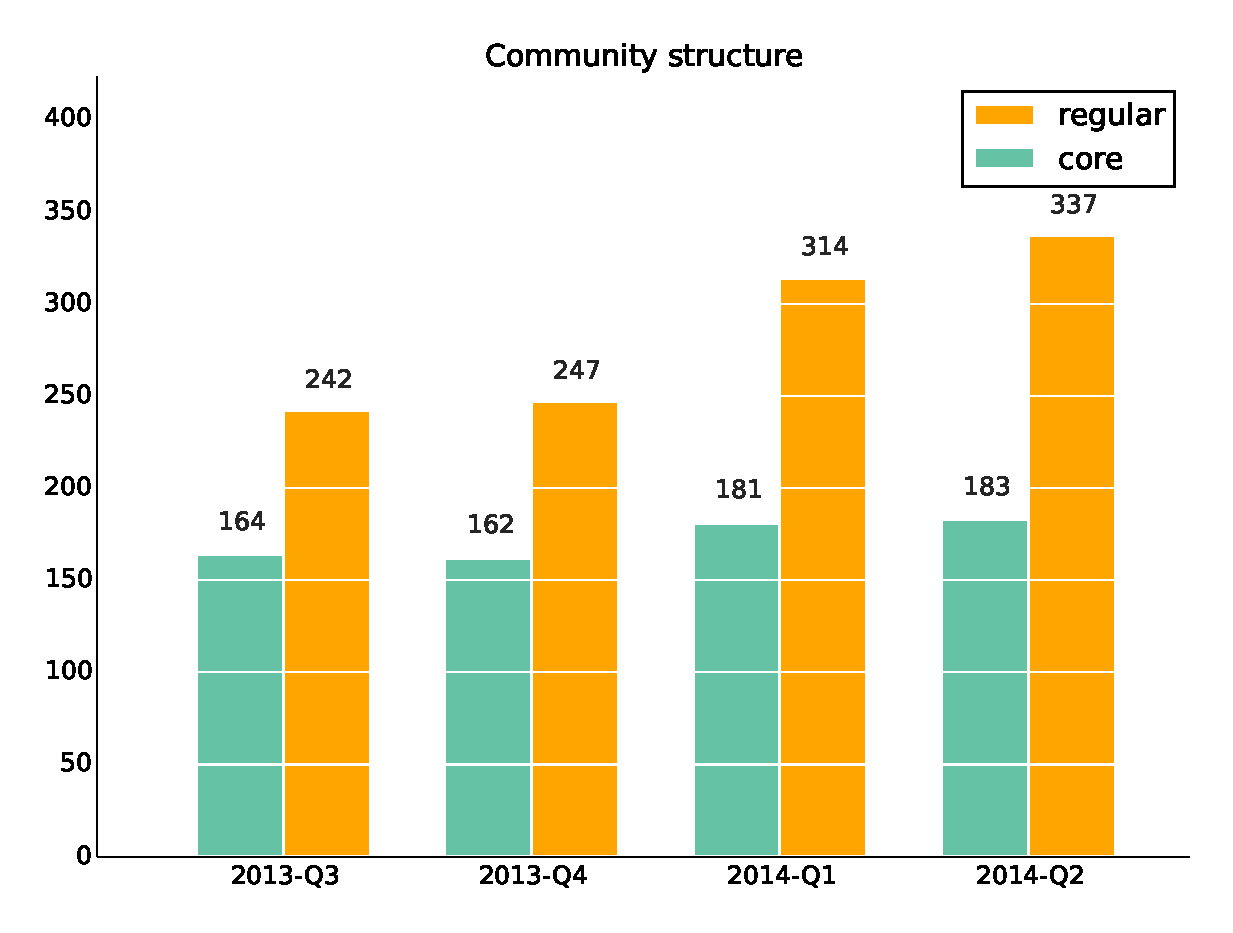
\includegraphics[scale=.35]{figs/onion.eps}
    \caption{Evolution of the last 4 quarters of the core, regular and occasional developers (Git activity)}
\end{figure}

\begin{table}[H]
    \centering
    \begin{tabular}{l|r|r|r|}%
    \bfseries Period & \bfseries Core & \bfseries Regular & \bfseries Occasional% specify table head
    \csvreader[head to column names]{data/onion_model.csv}{}% use head of csv as column names
    {\\\labels & \core & \regular & \occasional}
    \end{tabular}
    \caption{Characterization of developers by their total contribution to the OpenStack projects}
\end{table}


Although in the general overview, the mean number of developers participating per month has slightly decreased during the last quarter if compared to the first quarter of 2014.

\begin{figure}[H]
    \centering
    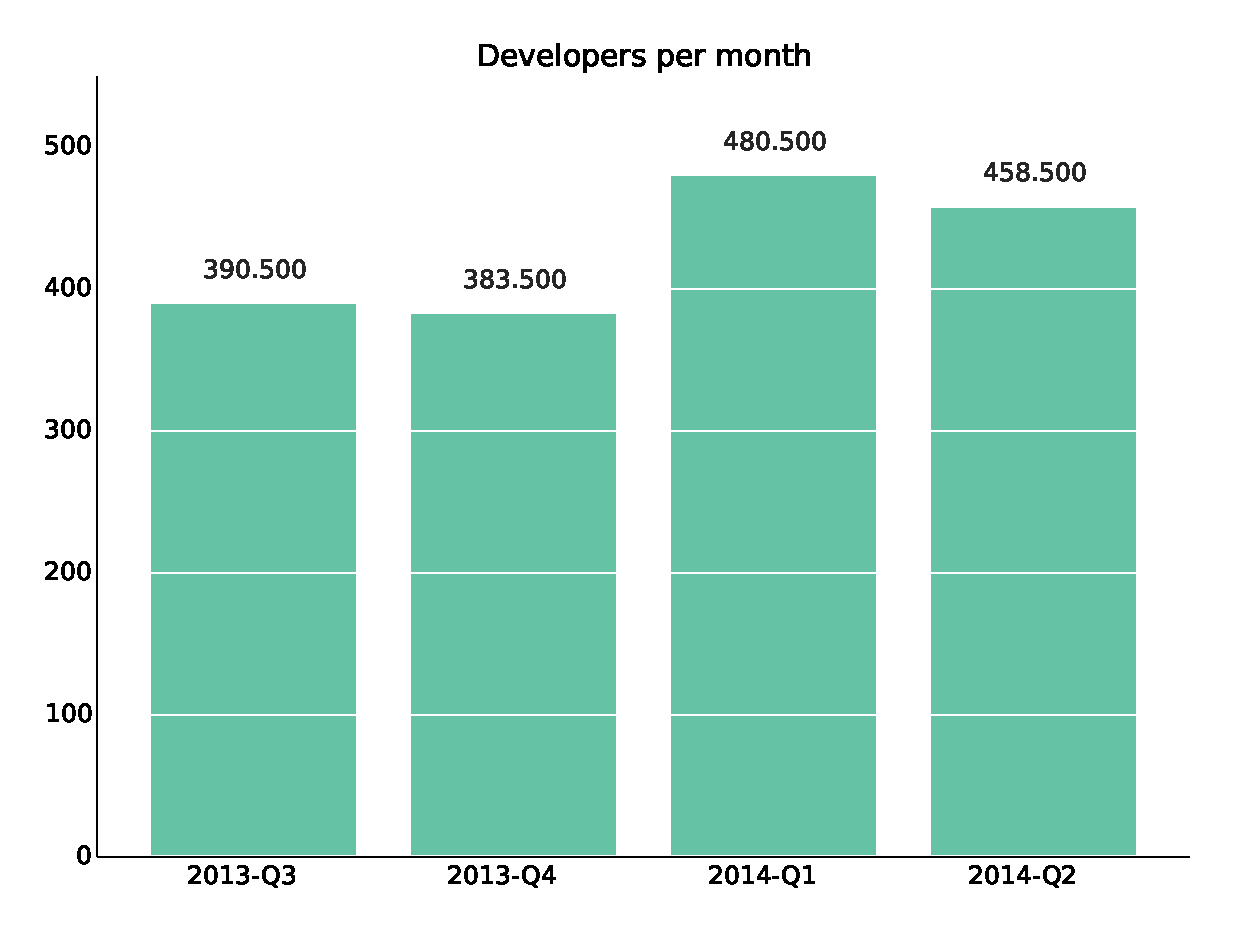
\includegraphics[scale=.35]{figs/authors_month.eps}
\caption{Number of developers per month in mean for each quarter}
\end{figure}

Regarding to main organizations participating in the development, those are listed based on information found on the git repositories. Two organizations (first and second in terms of commits) are identified per project\footnote{Integrated projects consist of the projects identified as integrated by the Programs yaml file available at \url{http://git.openstack.org/cgit/openstack/governance/tree/reference/programs.yaml} at the moment of this analysis}.


\begin{table}[H]
\centering
\begin{tabular}{c|r|} 
\textbf{Integrated project} & \textbf{Commits} \\
Nova & IBM / Rackspace\\
Neutron & Red Hat / VMware\\
Heat & Red Hat / Rackspace\\
Horizon & Red Hat / HP\\
Keystone & IBM / Rackspace\\
Cinder & Red Hat / HP\\
Sahara & Mirantis / Red Hat\\
Ceilometer & Mirantis / eNovance\\
Swift & Rackspace / Intel\\
Trove & HP / Rackspace\\
Glance & IBM / Red Hat\\
\end{tabular}
\caption{Organizations with the highest activity per integrated project}
\end{table}


In addition, the most active developers for each of the integrated projects are listed in the following table.


\begin{table}[H]
\centering
\begin{tabular}{c|r|} 
\textbf{Integrated project} & \textbf{Commits} \\
Nova & Dan Smith\\
Neutron & Kevin Benton\\
Heat & Zane Bitter\\
Horizon & julie Pichon\\
Keystone & Brant Knudson\\
Cinder & John Griffith\\
Sahara & Andrew Lazarev\\
Ceilometer & Mehdi Abaakouk\\
Swift & Clayg\\
Trove & Andreas Jaeger\\
Glance & Zhi Yan Liu\\
\end{tabular}
\caption{Top developers in commits per integrated project}
\end{table}


In terms of technical discussions and focus of interest in the community, main threads were 
focused on the interaction of Neutron and Barbican. First thread initiated by Jorge Miramontes on the 6th of June,  2014\footnote{\url{http://lists.openstack.org/pipermail/openstack-dev/2014-June/036937.html}}. This thread contains up
to 60 messages at the moment of this analysis. From the top 3 threads with the highest number of messages, two of them were
sent to the openstack-dev mailing list (60 and 42 messages), while the third one was sent to the openstack-operators mailing lists (48 messages).

Focusing on the number of different people involved in a thread, the thread initiated during the last quarter
with the highest number of participants is focused on Nova. 23 developers participated in the discussion with subject: "[openstack-dev][Nova] Thoughts from the PTL"\footnote{\url{http://lists.openstack.org/pipermail/openstack-dev/2014-April/032566.html}}. 

%Top tags missing information!
%Top questions in qa forums missing!

\section{Efficiency}



%Difference between integrated and non-integrated projects in terms of efficiency closing issues, and time to review, mean and median.

%Areas of knowledge per company in the integrated projects.

%Newer projects tend to be faster closing issues, or at least, they are improving their times to review and attend tickets. 

Two metrics have been identified to measure efficiency: the backlog management index (BMI) and the time to review. BMI is measured as the number of closed issues out of the opened issues in a given period. Time to review is measured as the time since a review is submitted till this
is closed. Typical BMI values in the OpenStack Integrated projects rounds a 0.6, what indicates that for 100 opened issues in a period, the community closes 60. Besides, the median time to review is of 6.81 days. Although other groups show a better
performance such as the Infrastructure with around 3 days of total time to review in median (10.3 in mean) those seem to show a lower performance in the BMI factor. In the case of the Infrastructure project, the BMI is around 0.12.


\begin{table}[H]
\centering
\begin{tabular}{c|r|r|} 
\textbf{Projects} & \textbf{BMI} & \textbf{Time to review (median)} \\
Integrated &  0.56 & 6.81 days\\
Incubated & 0.59 & 7.94 days\\
Clients & 0.65 & 10.43 days\\
Others & 0.75 & 5.06 days\\
Common Libraries & 0.66 & 6.17 days\\
Deployment & 0.75 & 11.68 days\\
Devstack & 0.08 & 3.11 days\\
Documentation & 0.04 & 0.54 days\\
Infrastructure & 0.12 & 3.07 days\\
Quality Assurance & 0.06 & 13.17 days\\
\end{tabular}
\caption{Closed issues out of opened issues (Launchpad tickets) and median time to review (Gerrit)}
\end{table}

And a detailed view of the evolution of the BMI during the last four quarters.

\begin{figure}[H]
\centering
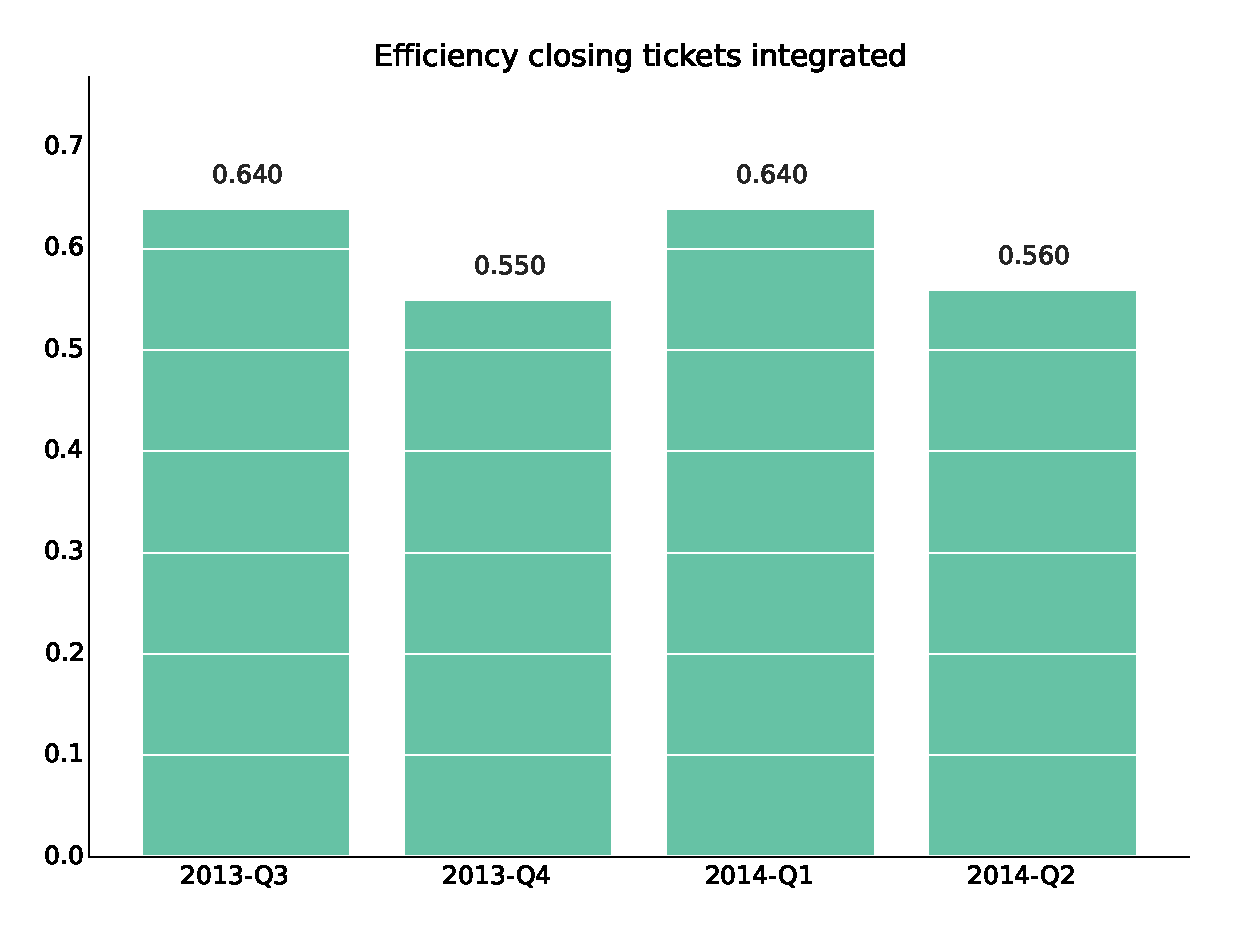
\includegraphics[scale=.35]{figs/bmiintegrated.eps}
\caption{Backlog Management Index evolution for the Integrated projects}
\end{figure}


%However, these numbers show that there is a gap of pending tickets opened that can be visualized at\footnote{dashboard url}. 

%Best project closing issues (with the best efficiency)
%Best project with the time to review
%Company leading most of the projects
%Projects with the highest number of developers

%Comparison of the activity of qaforums and mailing lists (qaforums is increasing, while mailing lists keep stable).

%Top threads (crowdest and with the highest number of issues)
%Top tags (topics) mentioned in the qaforums stuff
%Top visited questions and top commented questions from qaforums.


\chapter{Per Project break down}

This chapter aims at providing a detailed report on the activity of the OpenStack Foundation projects.
This is mainly focused on the activity per project as defined, stressing the point on the 'integrated' projects.

Each of the projects is divided into three sections and provides information from the last four quarters.: 
\begin{itemize}
\item activity: centered in the following metrics: commits from git activity, submitted, merge and abandoned reviews from the review system and
opened and closed tickets from the issue tracking system. 
\item community: focused on the total number of authors per quarter, top ten developers and top ten organizations contributing to the development
of each project.
\item process: centered on the analysis of how efficient is the community dealing with issues and reviews.
\end{itemize}


\section{Overall OpenStack Programms}

\textbf{Activity}: Commits in Git, submitted, merged and abandoned reviews in Gerrit and opened and closed issues in Launchpad.

\begin{tabular}{p{7cm} p{5cm}}
    \vspace{0pt} 
    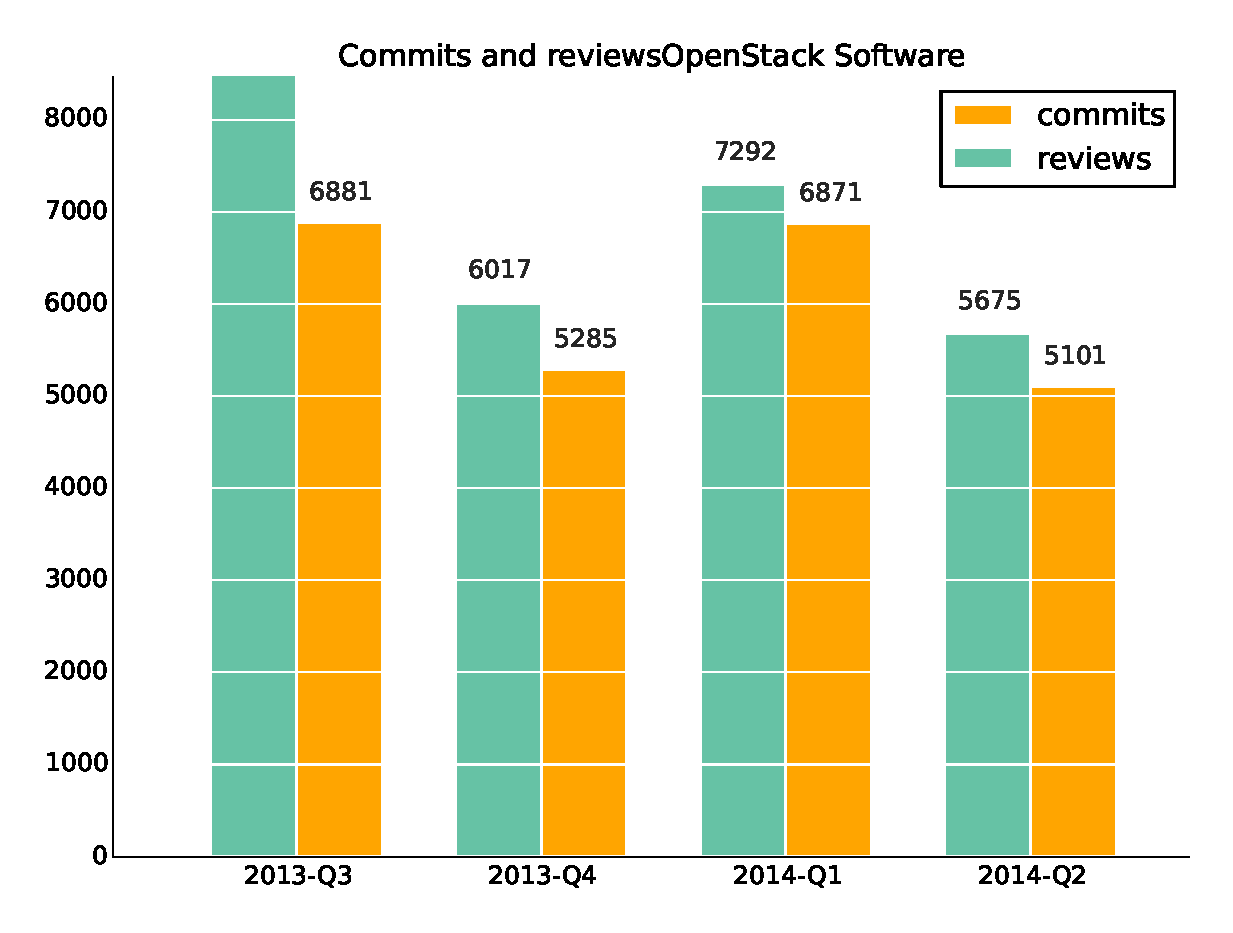
\includegraphics[scale=.35]{figs/commitsOpenStackSoftware.eps}
    & 
    \vspace{0pt}
    \begin{tabular}{l|r|r|}%
    \bfseries Period & \bfseries Commits & \bfseries Reviews% specify table head
    \csvreader[head to column names]{data/commitsOpenStackSoftware.csv}{}% use head of csv as column names
    {\\\labels & \commits & \submitted}
    \end{tabular}
\end{tabular}


\begin{tabular}{p{7cm} p{5cm}}
    \vspace{0pt} 
    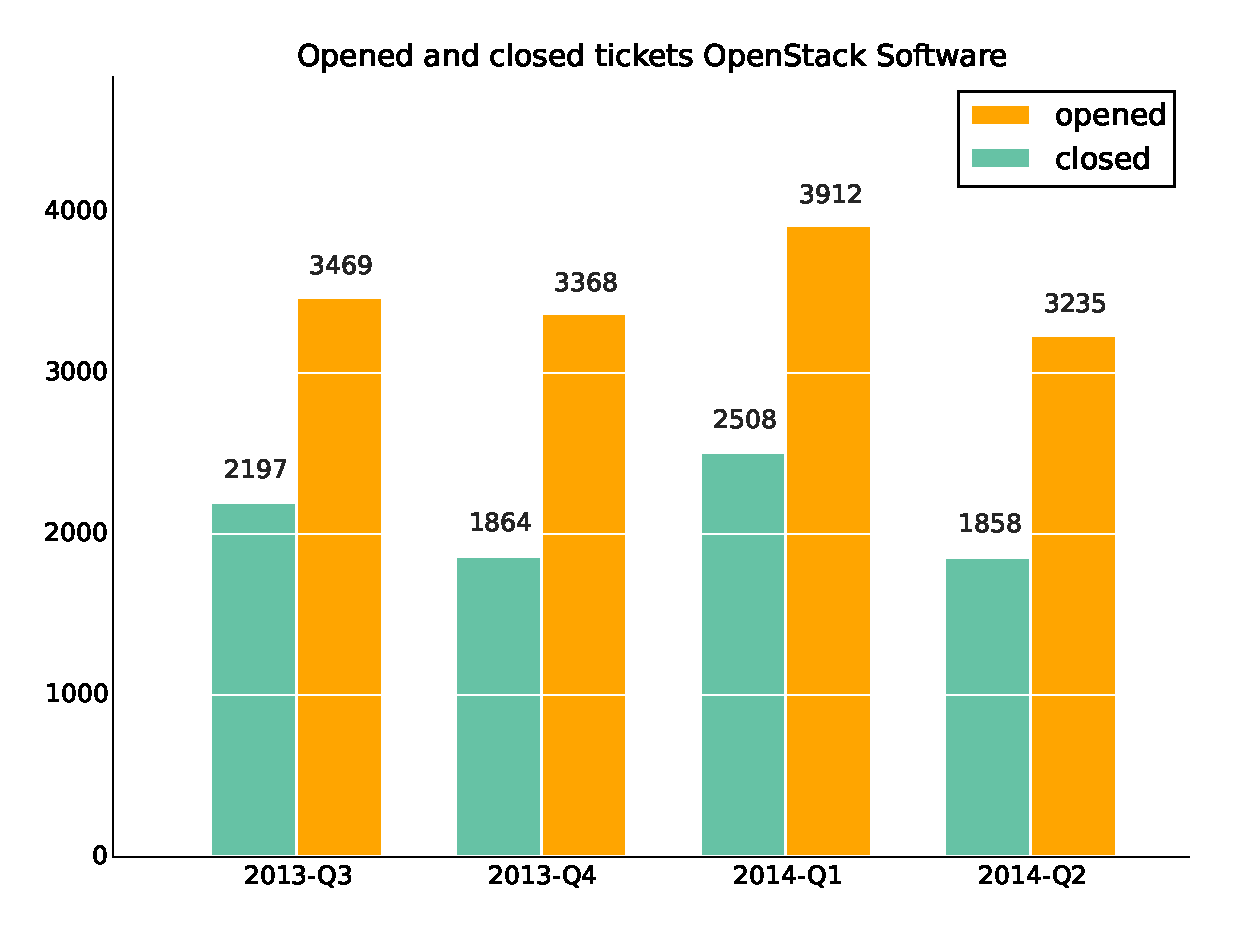
\includegraphics[scale=.35]{figs/closedOpenStackSoftware.eps}
    & 
    \vspace{0pt}
    \begin{tabular}{l|r|r|}%
    \bfseries Period & \bfseries Closed & \bfseries Opened% specify table head
    \csvreader[head to column names]{data/closedOpenStackSoftware.csv}{}% use head of csv as column names
    {\\\labels & \closed & \opened}
    \end{tabular}
\end{tabular}

\begin{tabular}{p{7cm} p{5cm}}
    \vspace{0pt} 
    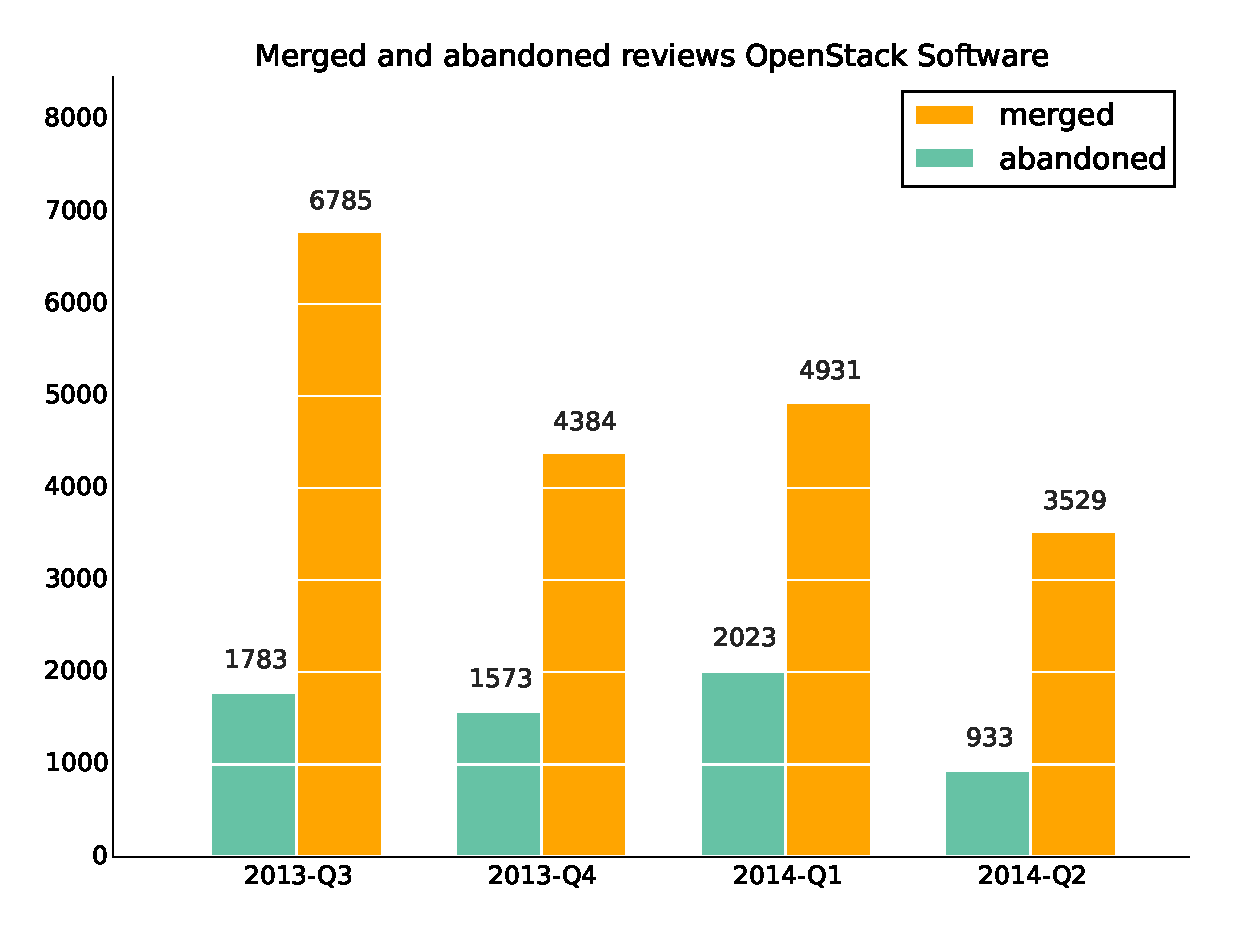
\includegraphics[scale=.35]{figs/submitted_reviewsOpenStackSoftware.eps}
    & 
    \vspace{0pt}
    \begin{tabular}{l|r|r|}%
    \bfseries Period & \bfseries Merged & \bfseries Abandoned % specify table head
    \csvreader[head to column names]{data/submitted_reviewsOpenStackSoftware.csv}{}% use head of csv as column names
    {\\\labels & \merged & \abandoned}
    \end{tabular}
\end{tabular}

\textbf{Community}: Authors per quarter and top authors and organizations in the last quarter

\begin{tabular}{p{7cm} p{5cm}}
    \vspace{0pt} 
    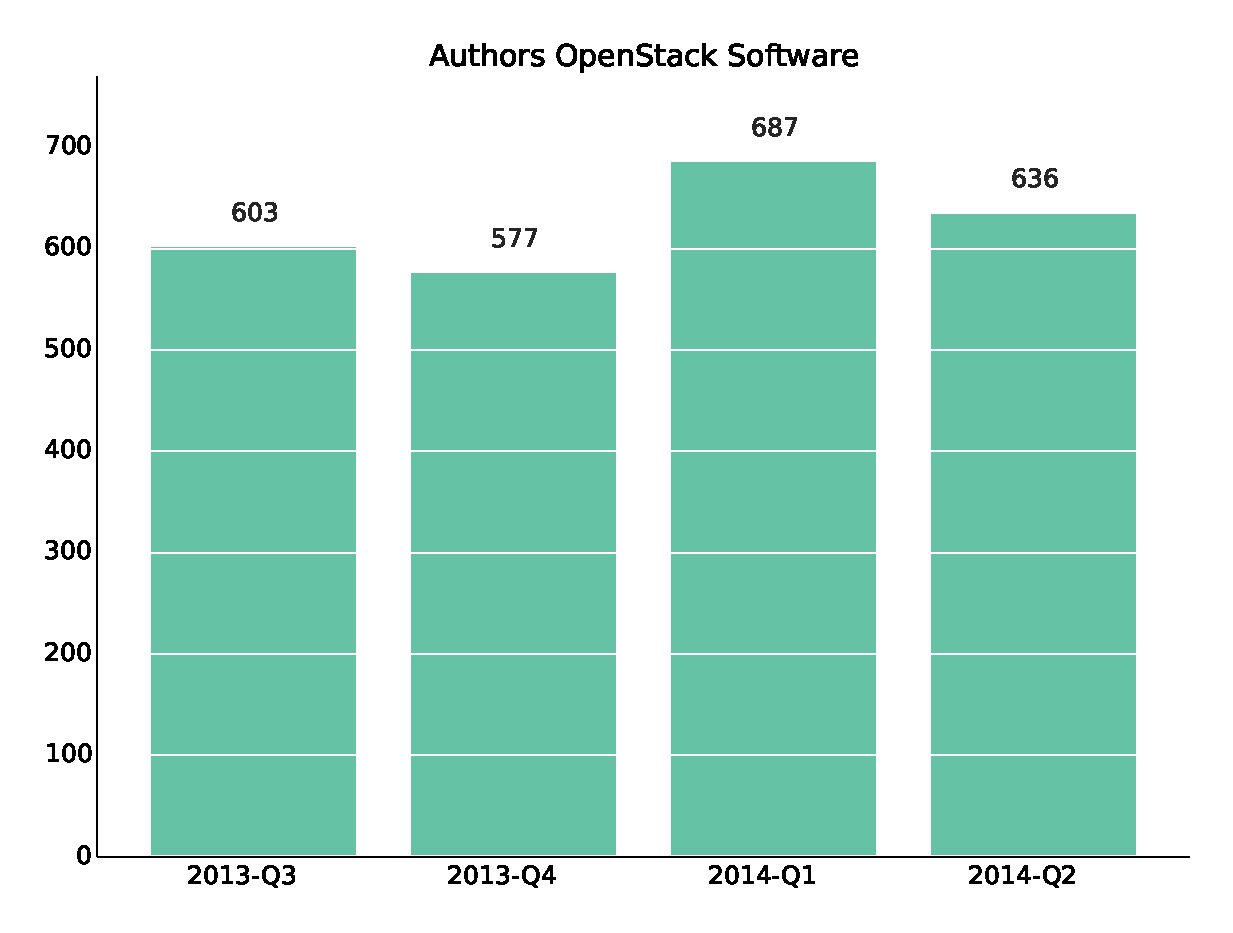
\includegraphics[scale=.35]{figs/authorsOpenStackSoftware.eps}
    & 
    \vspace{0pt}
    \begin{tabular}{l|l}%
    \bfseries Period & \bfseries Authors % specify table head
    \csvreader[head to column names]{data/authorsOpenStackSoftware.csv}{}% use head of csv as column names
    {\\\labels & \authors}
    \end{tabular}
\end{tabular}

\begin{tabular}{p{7cm} p{5cm}}
    \vspace{0pt}
\begin{tabular}{l|l}%
    \bfseries Commit (s) & \bfseries Author % specify table head
    \csvreader[head to column names]{data/scm_top_authors_project_OpenStackSoftware.csv}{}% use head of csv as column names
    {\\\hline\csvcoli&\csvcolii}% specify your coloumns here
\end{tabular}
&
\vspace{0pt}
\begin{tabular}{l|l}%
    \bfseries Commit (s) & \bfseries Organizations % specify table head
    \csvreader[head to column names]{data/scm_top_companies_project_OpenStackSoftware.csv}{}% use head of csv as column names
    {\\\hline\csvcoli&\csvcolii}% specify your coloumns here
\end{tabular}
\end {tabular}


\textbf{Process}: Efficiency closing issues and time to review: mean and median

\begin{tabular}{p{7cm} p{5cm}}
    \vspace{0pt} 
    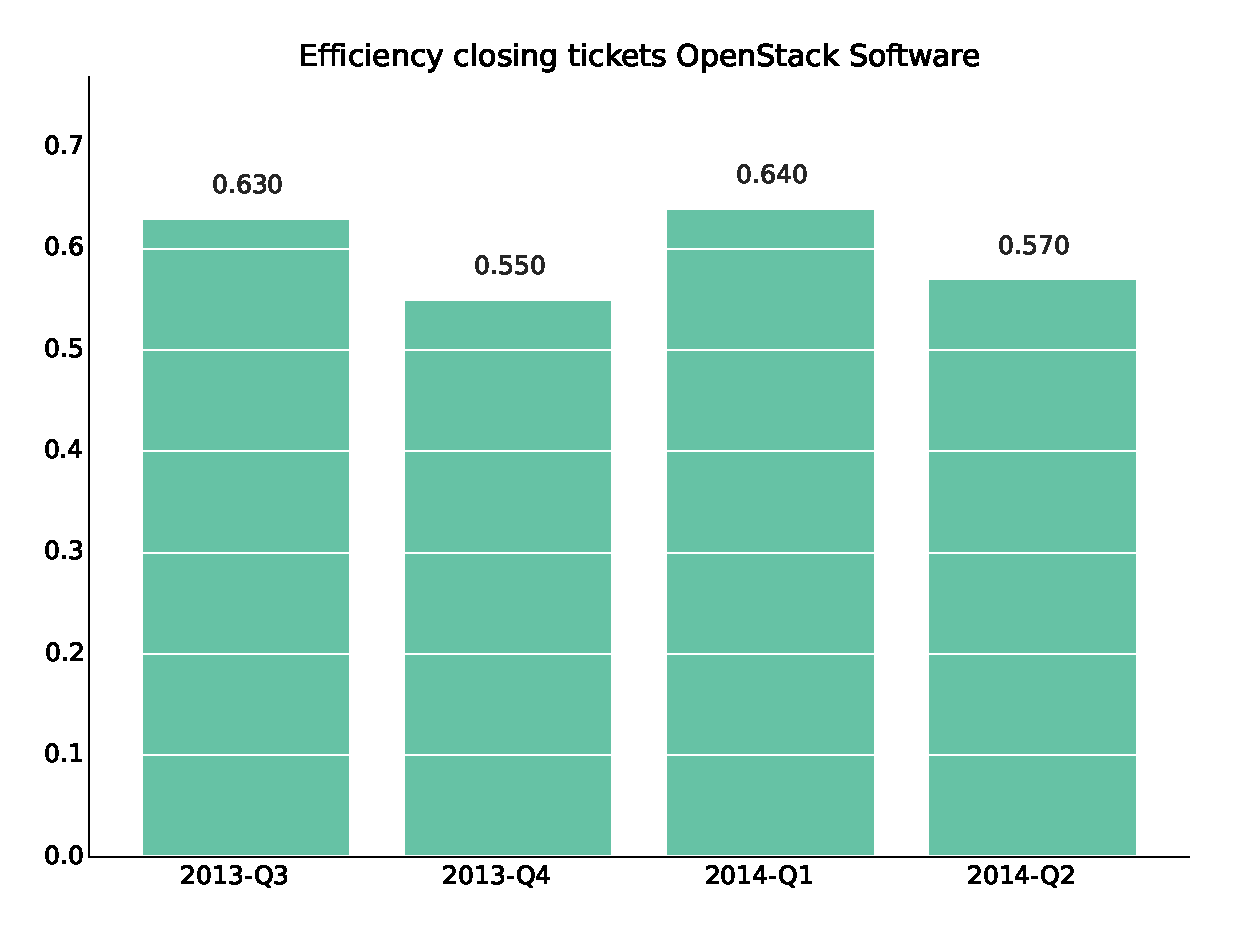
\includegraphics[scale=.35]{figs/bmiOpenStackSoftware.eps}
    & 
    \vspace{0pt}
    \begin{tabular}{l|l}%
    \bfseries Period & \bfseries Closed/Opened % specify table head
    \csvreader[head to column names]{data/bmiOpenStackSoftware.csv}{}% use head of csv as column names
    {\\\labels & \bmi}
    \end{tabular}
\end{tabular}

\begin{tabular}{p{7cm} p{5cm}}
    \vspace{0pt} 
    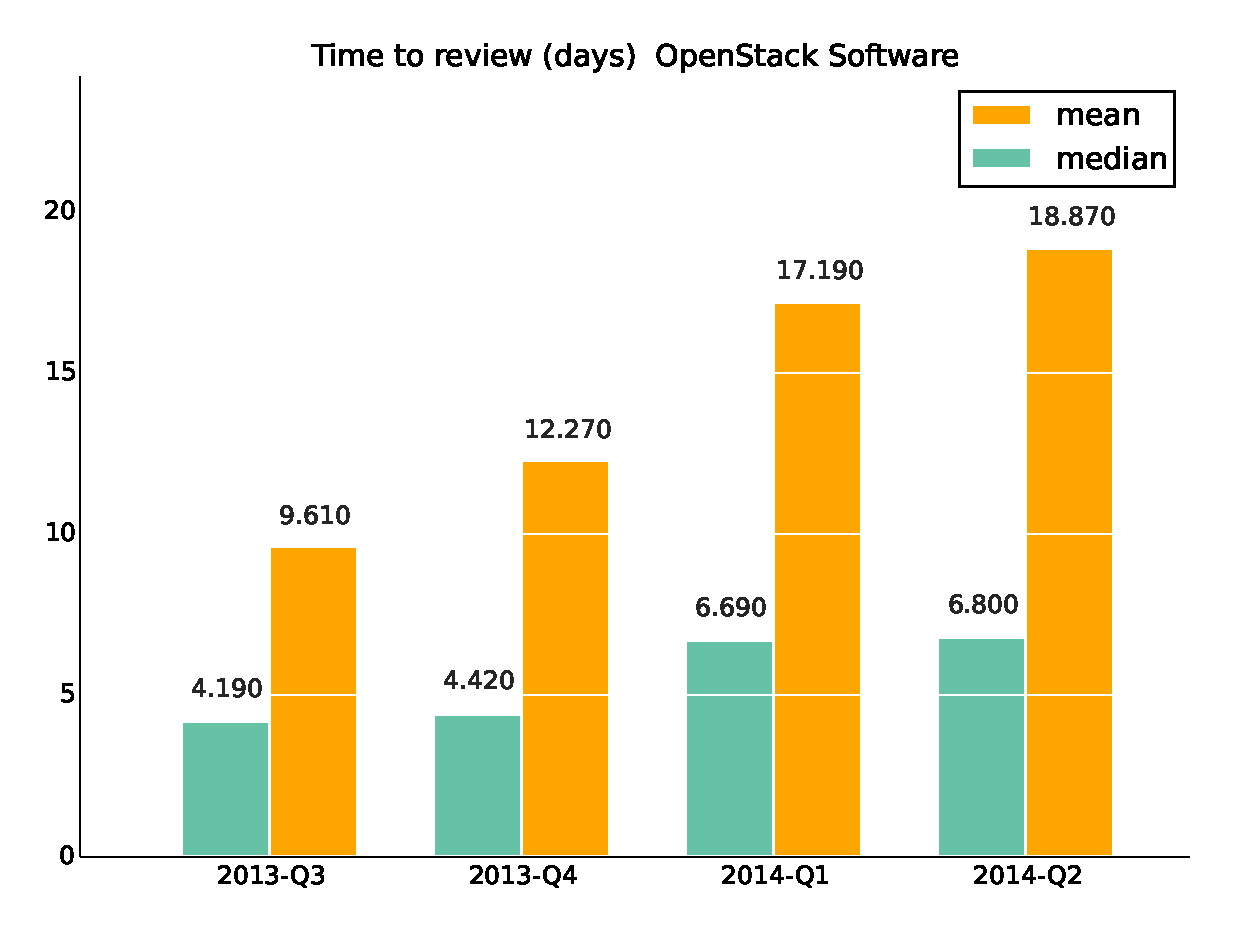
\includegraphics[scale=.35]{figs/timetoreview_medianOpenStackSoftware.eps}
    & 
    \vspace{0pt}
    \begin{tabular}{l|r|r|}%
    \bfseries Period & \bfseries Median & \bfseries Mean % specify table head
    \csvreader[head to column names]{data/timetoreview_medianOpenStackSoftware.csv}{}% use head of csv as column names
    {\\\labels & \mediantime & \meantime}
    \end{tabular}
\end{tabular}

\newpage

\subsection{OpenStack Integrated Programs}

\textbf{Activity}: Commits in Git, submitted, merged and abandoned reviews in Gerrit and opened and closed issues in Launchpad.

\begin{tabular}{p{7cm} p{5cm}}
    \vspace{0pt} 
    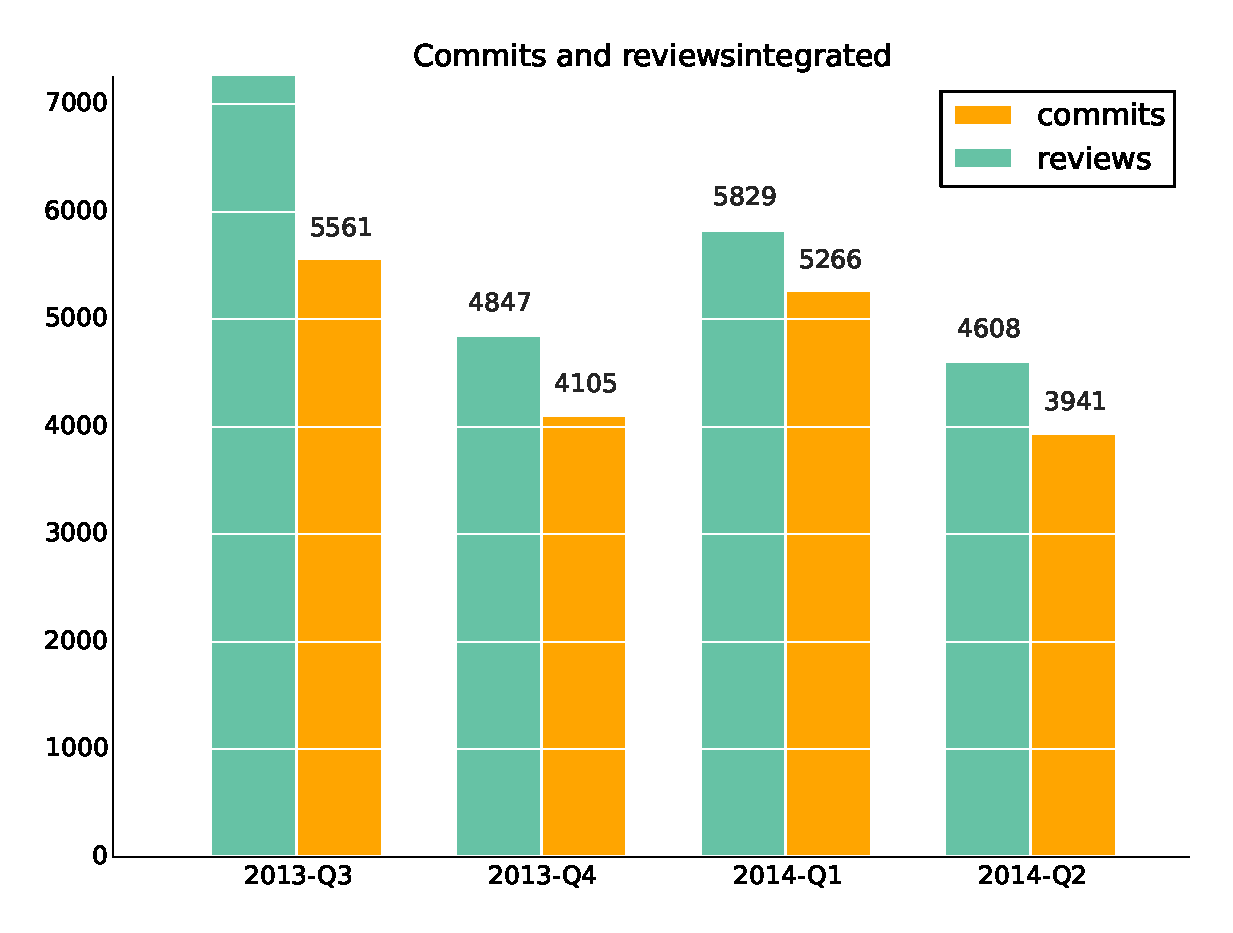
\includegraphics[scale=.35]{figs/commitsintegrated.eps}
    & 
    \vspace{0pt}
    \begin{tabular}{l|r|r|}%
    \bfseries Period & \bfseries Commits & \bfseries Reviews% specify table head
    \csvreader[head to column names]{data/commitsintegrated.csv}{}% use head of csv as column names
    {\\\labels & \commits & \submitted}
    \end{tabular}
\end{tabular}

\begin{tabular}{p{7cm} p{5cm}}
    \vspace{0pt} 
    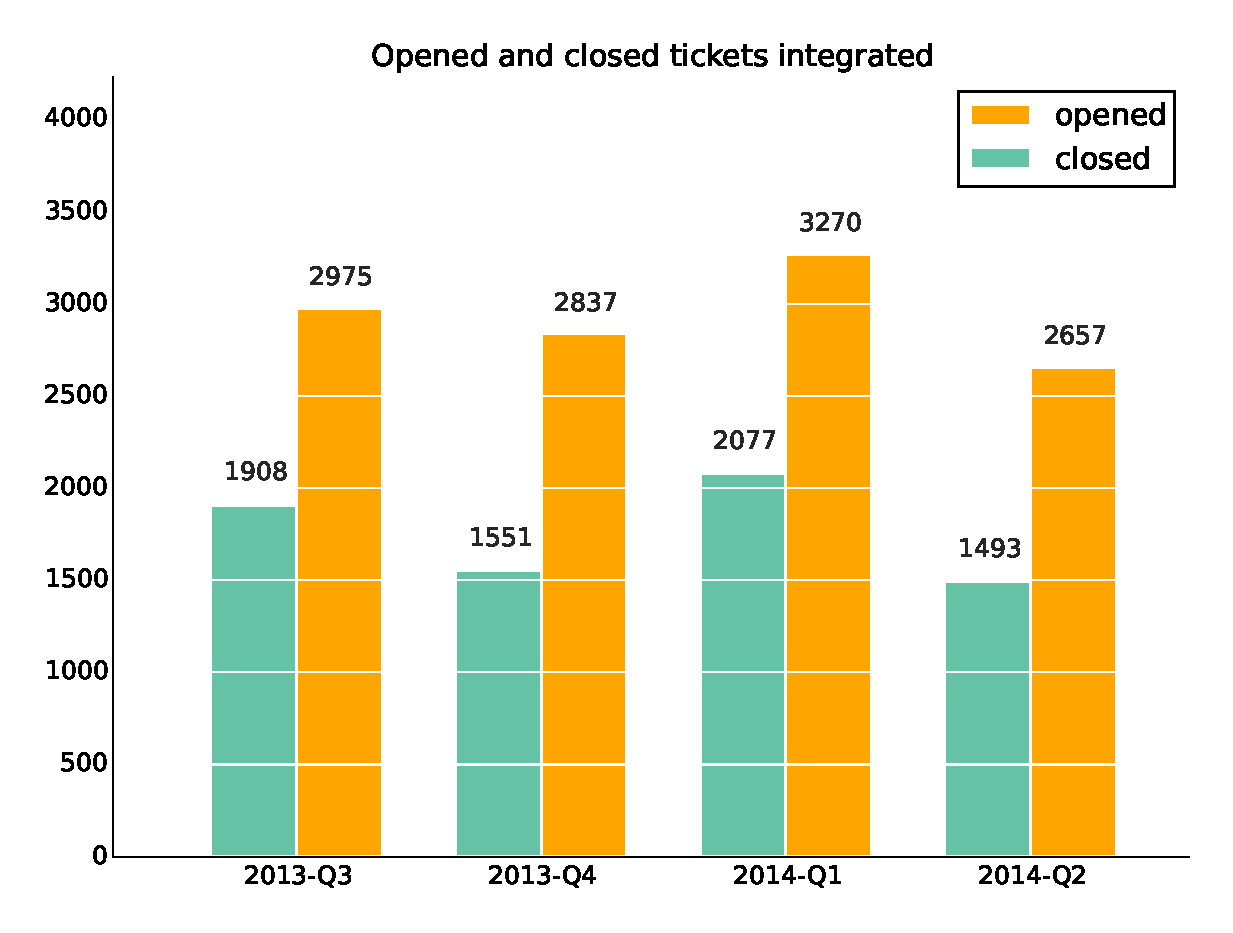
\includegraphics[scale=.35]{figs/closedintegrated.eps}
    & 
    \vspace{0pt}
    \begin{tabular}{l|r|r|}%
    \bfseries Period & \bfseries Closed & \bfseries Opened% specify table head
    \csvreader[head to column names]{data/closedintegrated.csv}{}% use head of csv as column names
    {\\\labels & \closed & \opened}
    \end{tabular}
\end{tabular}

\begin{tabular}{p{7cm} p{5cm}}
    \vspace{0pt} 
    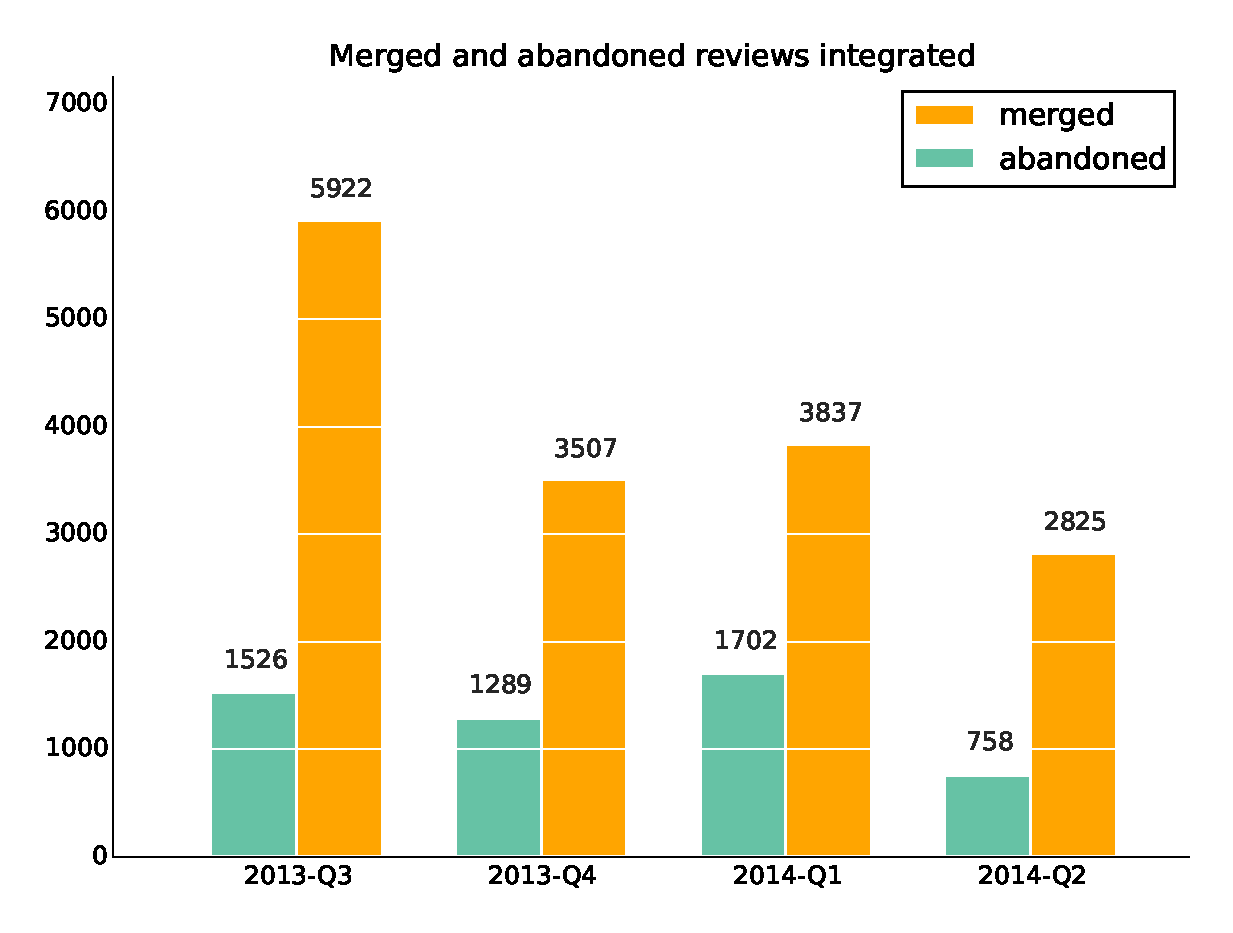
\includegraphics[scale=.35]{figs/submitted_reviewsintegrated.eps}
    & 
    \vspace{0pt}
    \begin{tabular}{l|r|r|}%
    \bfseries Period & \bfseries Merged & \bfseries Abandoned % specify table head
    \csvreader[head to column names]{data/submitted_reviewsintegrated.csv}{}% use head of csv as column names
    {\\\labels & \merged & \abandoned}
    \end{tabular}
\end{tabular}


\textbf{Community}: Authors per quarter and top authors and organizations in the last quarter

\begin{tabular}{p{7cm} p{5cm}}
    \vspace{0pt} 
    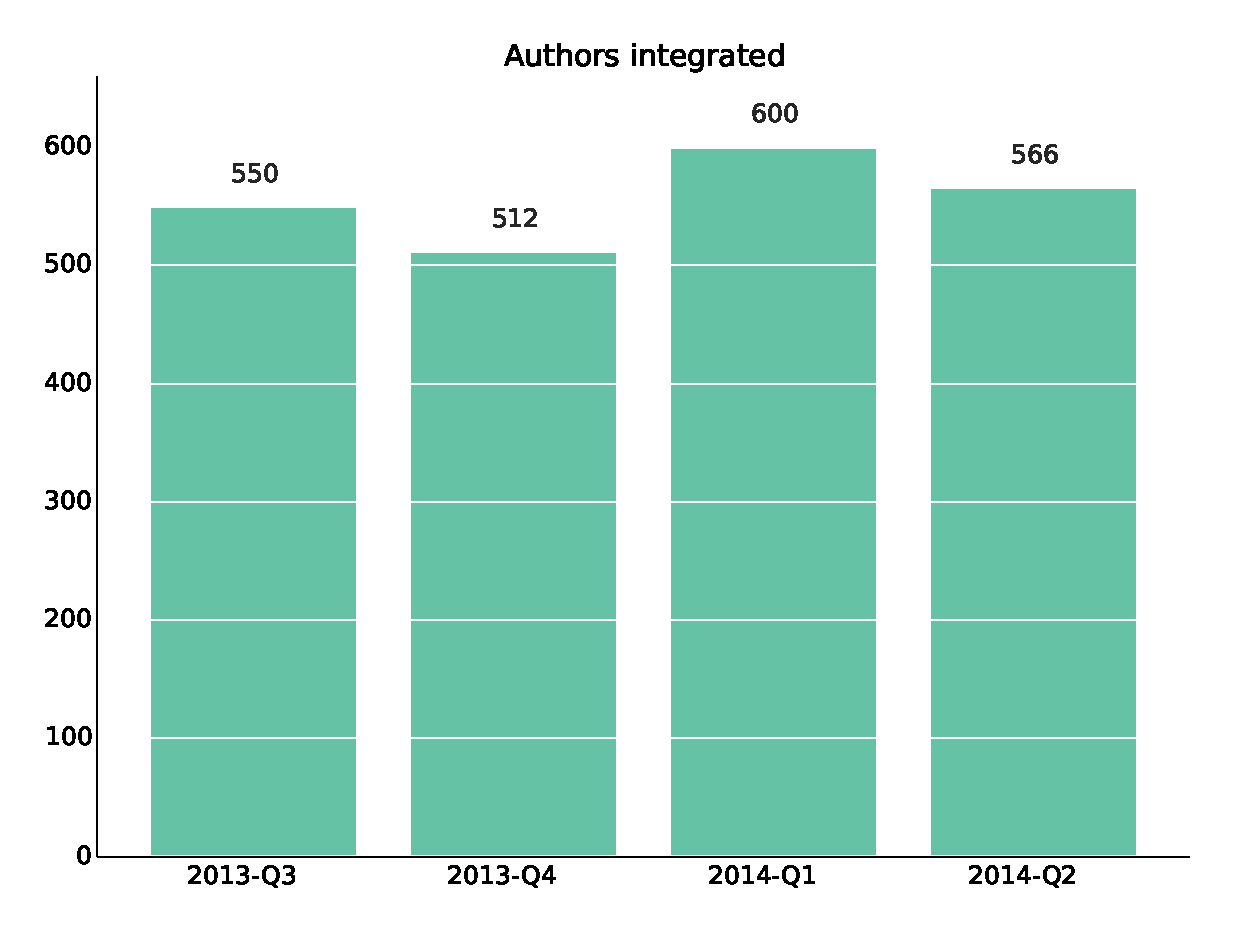
\includegraphics[scale=.35]{figs/authorsintegrated.eps}
    & 
    \vspace{0pt}
    \begin{tabular}{l|l}%
    \bfseries Period & \bfseries Authors % specify table head
    \csvreader[head to column names]{data/authorsintegrated.csv}{}% use head of csv as column names
    {\\\labels & \authors}
    \end{tabular}
\end{tabular}

\begin{tabular}{p{7cm} p{5cm}}
    \vspace{0pt}
\begin{tabular}{l|l}%
    \bfseries Commit (s) & \bfseries Author % specify table head
    \csvreader[head to column names]{data/scm_top_authors_project_integrated.csv}{}% use head of csv as column names
    {\\\hline\csvcoli&\csvcolii}% specify your coloumns here
\end{tabular}
&
\vspace{0pt}
\begin{tabular}{l|l}%
    \bfseries Commit (s) & \bfseries Organizations % specify table head
    \csvreader[head to column names]{data/scm_top_companies_project_integrated.csv}{}% use head of csv as column names
    {\\\hline\csvcoli&\csvcolii}% specify your coloumns here
\end{tabular}
\end {tabular}


\textbf{Process}: Efficiency closing issues and time to review: mean and median

\begin{tabular}{p{7cm} p{5cm}}
    \vspace{0pt} 
    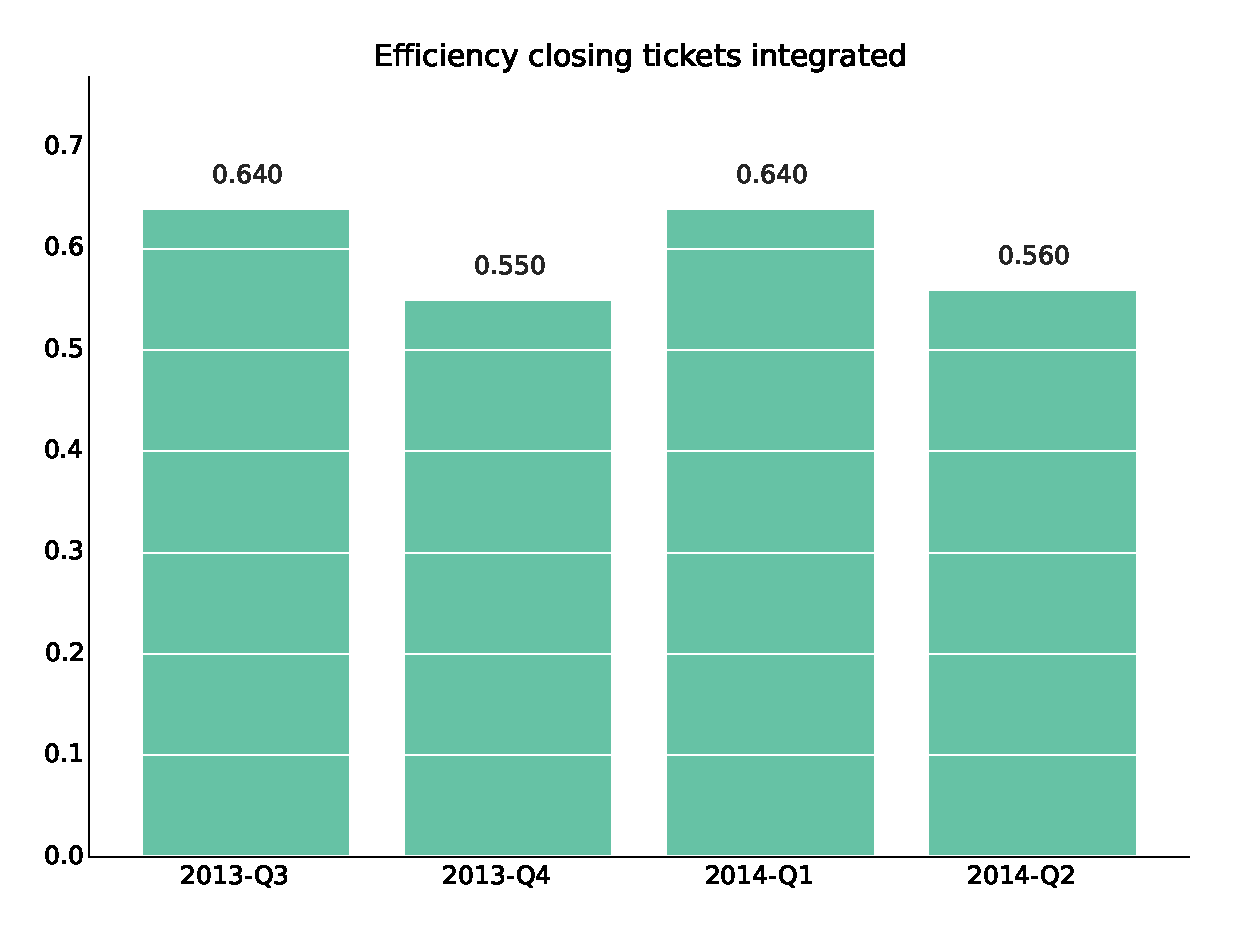
\includegraphics[scale=.35]{figs/bmiintegrated.eps}
    & 
    \vspace{0pt}
    \begin{tabular}{l|l}%
    \bfseries Period & \bfseries Closed/Opened % specify table head
    \csvreader[head to column names]{data/bmiintegrated.csv}{}% use head of csv as column names
    {\\\labels & \bmi}
    \end{tabular}
\end{tabular}

\begin{tabular}{p{7cm} p{5cm}}
    \vspace{0pt} 
    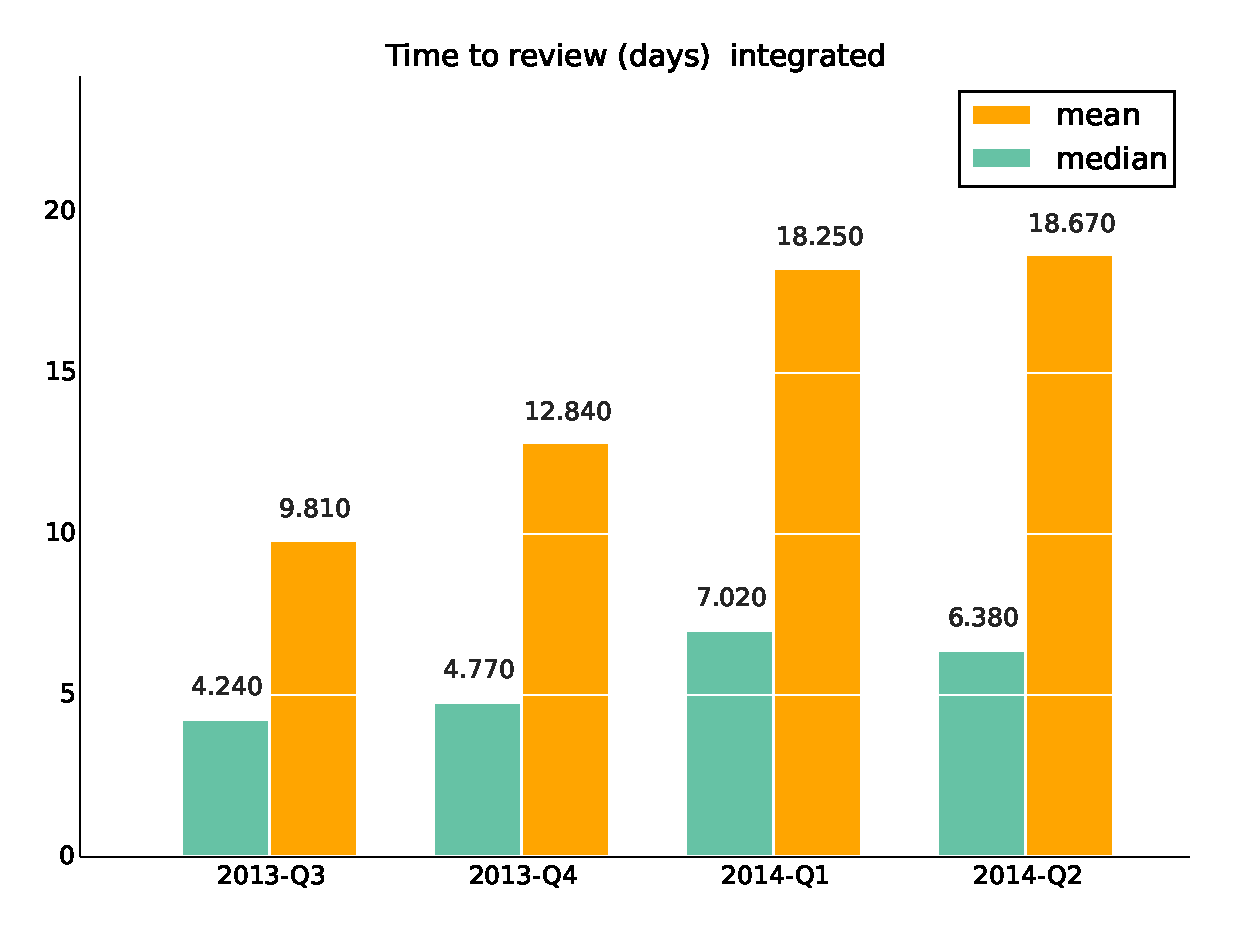
\includegraphics[scale=.35]{figs/timetoreview_medianintegrated.eps}
    & 
    \vspace{0pt}
    \begin{tabular}{l|r|r|}%
    \bfseries Period & \bfseries Median & \bfseries Mean % specify table head
    \csvreader[head to column names]{data/timetoreview_medianintegrated.csv}{}% use head of csv as column names
    {\\\labels & \mediantime & \meantime}
    \end{tabular}
\end{tabular}

\newpage 
 \subsubsection{Ceilometer}

\textbf{Activity}: Commits in Git, submitted, merged and abandoned reviews in Gerrit and opened and closed issues in Launchpad.

\begin{tabular}{p{7cm} p{5cm}}
    \vspace{0pt} 
    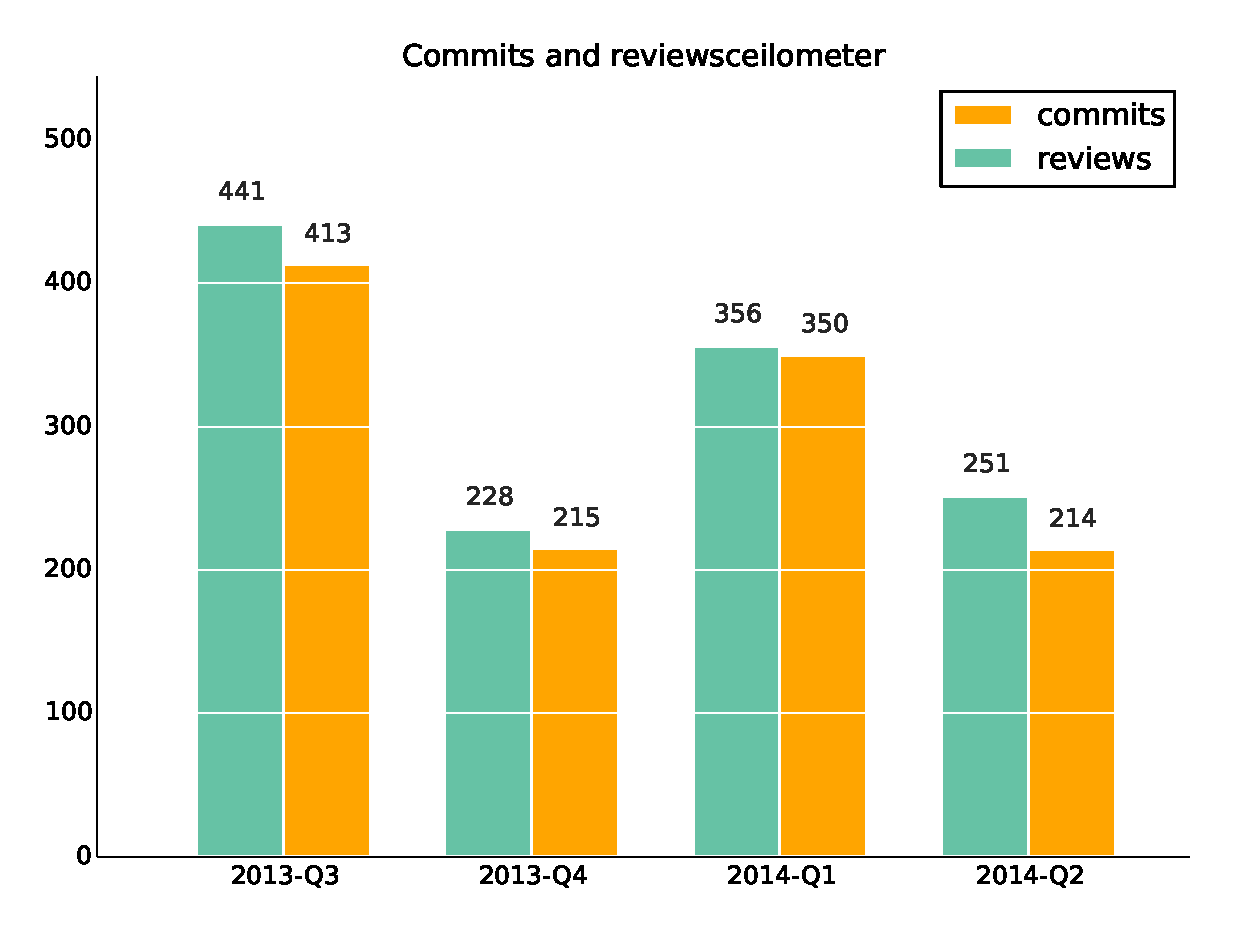
\includegraphics[scale=.35]{figs/commitsceilometer.eps}
    & 
    \vspace{0pt}
    \begin{tabular}{l|r|r|}%
    \bfseries Period & \bfseries Commits & \bfseries Reviews % specify table head
    \csvreader[head to column names]{data/commitsceilometer.csv}{}% use head of csv as column names
    {\\\labels & \commits & \submitted}
    \end{tabular}
\end{tabular}

\begin{tabular}{p{7cm} p{5cm}}
    \vspace{0pt} 
    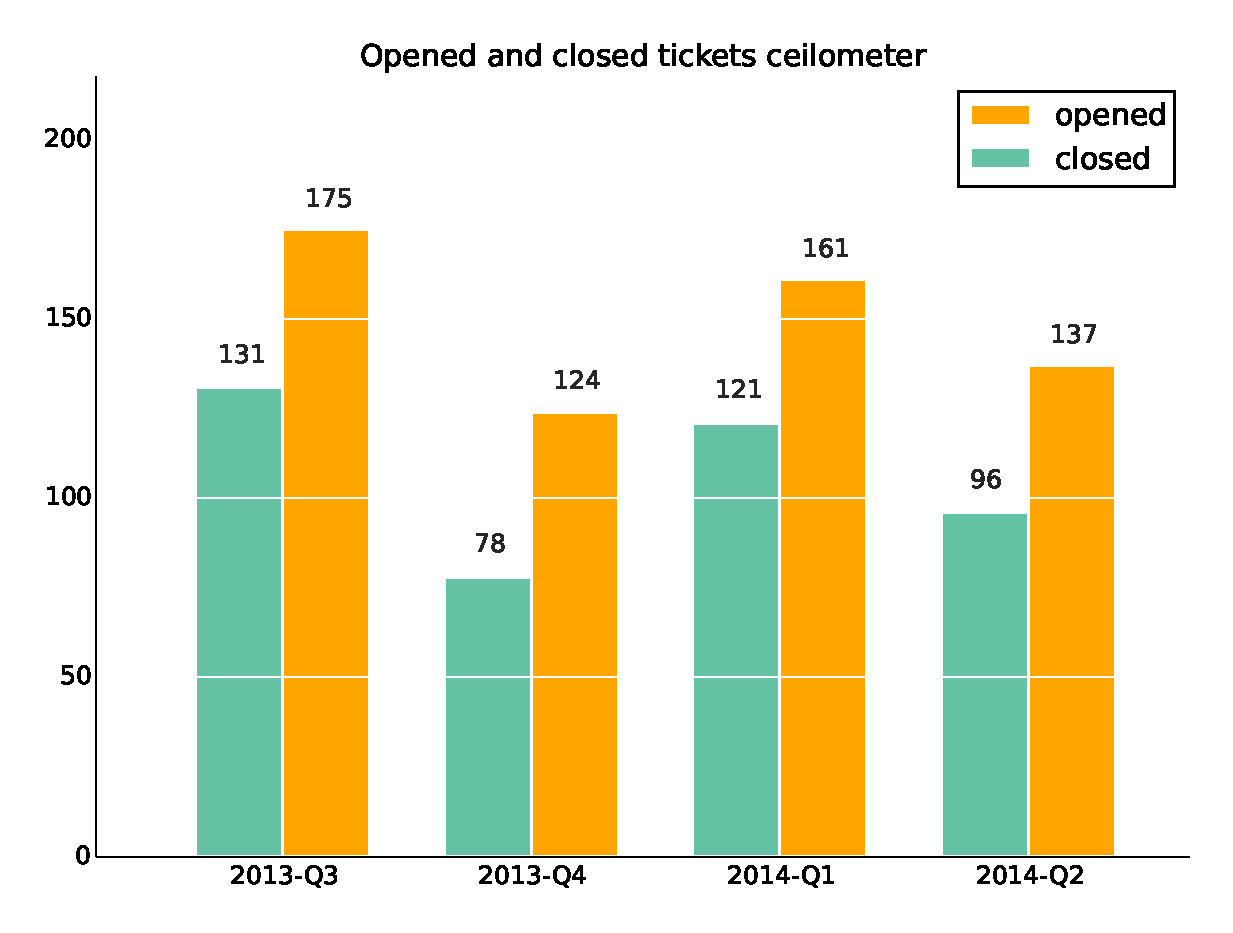
\includegraphics[scale=.35]{figs/closedceilometer.eps}
    & 
    \vspace{0pt}
    \begin{tabular}{l|r|r|}%
    \bfseries Period & \bfseries Closed & \bfseries Opened
    \csvreader[head to column names]{data/closedceilometer.csv}{}% use head of csv as column names
    {\\\labels & \closed & \opened}
    \end{tabular}
\end{tabular}

\begin{tabular}{p{7cm} p{5cm}}
    \vspace{0pt} 
    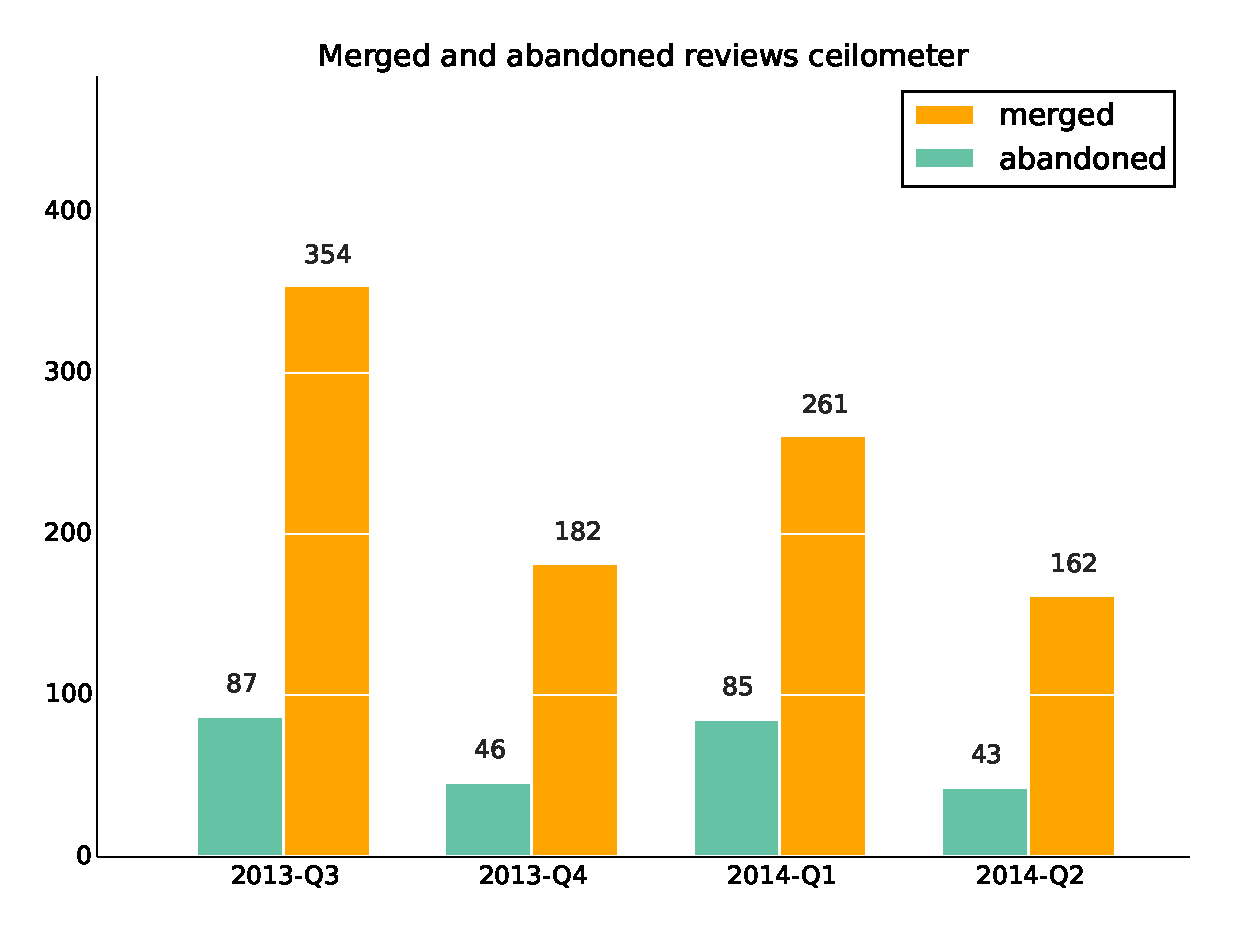
\includegraphics[scale=.35]{figs/submitted_reviewsceilometer.eps}
    & 
    \vspace{0pt}
    \begin{tabular}{l|r|r|}%
    \bfseries Period & \bfseries Merged & \bfseries Abandoned % specify table head
    \csvreader[head to column names]{data/submitted_reviewsceilometer.csv}{}% use head of csv as column names
    {\\\labels & \merged & \abandoned}
    \end{tabular}
\end{tabular}


\textbf{Community}: Authors per quarter and top authors and organizations in the last quarter

\begin{tabular}{p{7cm} p{5cm}}
    \vspace{0pt} 
    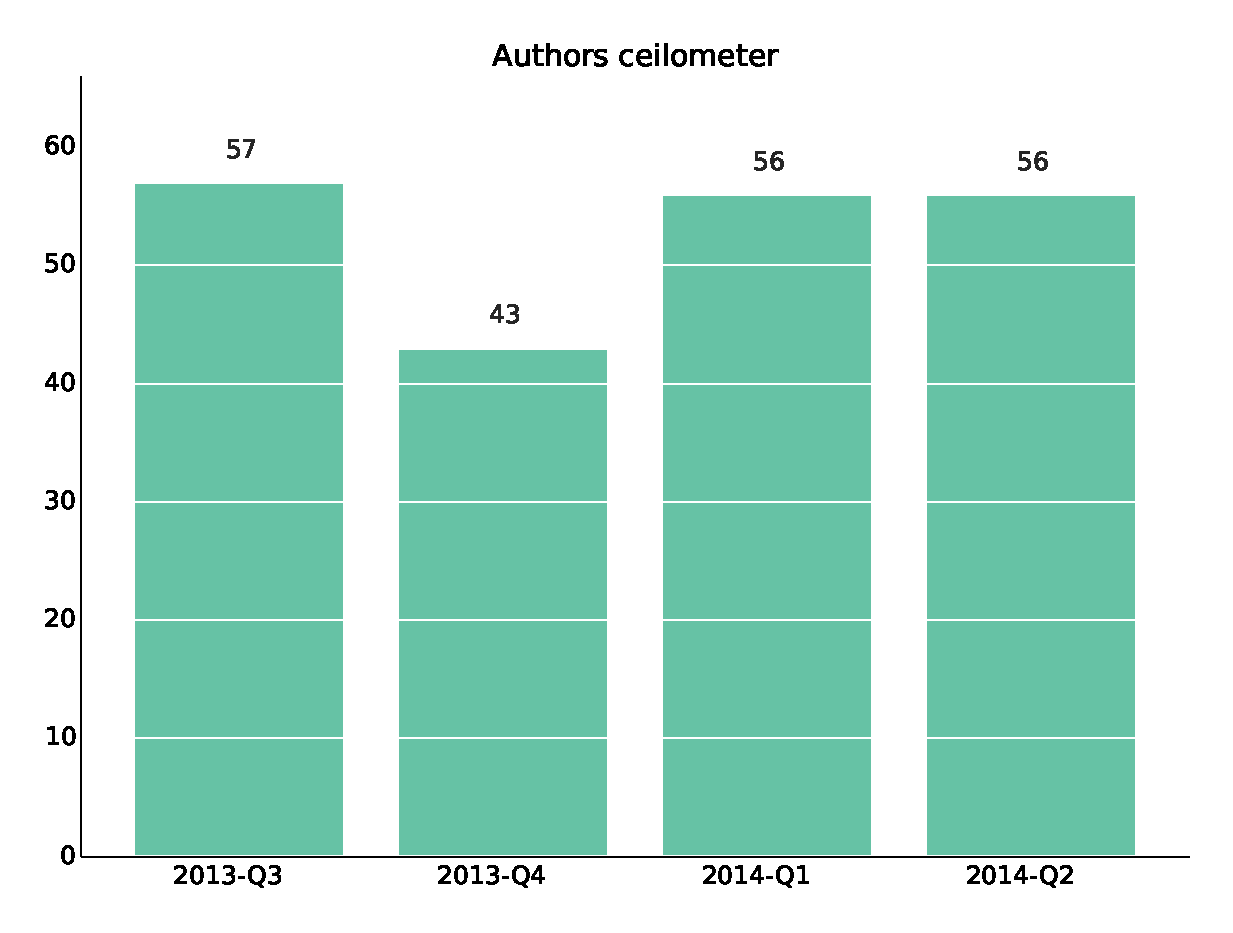
\includegraphics[scale=.35]{figs/authorsceilometer.eps}
    & 
    \vspace{0pt}
    \begin{tabular}{l|l}%
    \bfseries Period & \bfseries Authors % specify table head
    \csvreader[head to column names]{data/authorsceilometer.csv}{}% use head of csv as column names
    {\\\labels & \authors}
    \end{tabular}
\end{tabular}

\begin{tabular}{p{7cm} p{5cm}}
    \vspace{0pt}
\begin{tabular}{l|l}%
    \bfseries Commit (s) & \bfseries Author % specify table head
    \csvreader[head to column names]{data/scm_top_authors_project_ceilometer.csv}{}% use head of csv as column names
    {\\\hline\csvcoli&\csvcolii}% specify your coloumns here
\end{tabular}
&
\vspace{0pt}
\begin{tabular}{l|l}%
    \bfseries Commit (s) & \bfseries Organizations % specify table head
    \csvreader[head to column names]{data/scm_top_companies_project_ceilometer.csv}{}% use head of csv as column names
    {\\\hline\csvcoli&\csvcolii}% specify your coloumns here
\end{tabular}
\end {tabular}

\textbf{Process}: Efficiency closing issues and time to review: mean and median

\begin{tabular}{p{7cm} p{5cm}}
    \vspace{0pt} 
    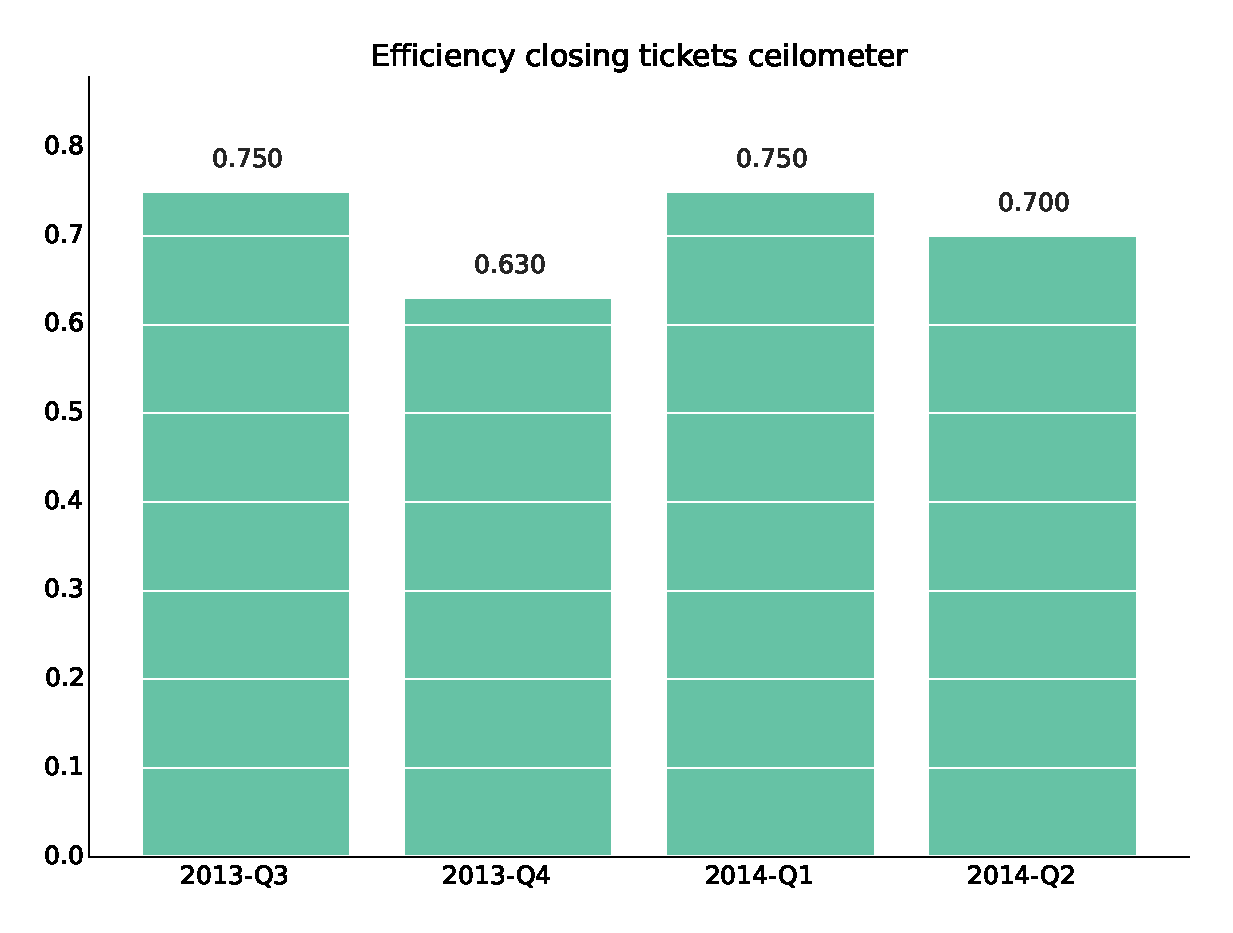
\includegraphics[scale=.35]{figs/bmiceilometer.eps}
    & 
    \vspace{0pt}
    \begin{tabular}{l|l}%
    \bfseries Period & \bfseries Closed/Opened % specify table head
    \csvreader[head to column names]{data/bmiceilometer.csv}{}% use head of csv as column names
    {\\\labels & \bmi}
    \end{tabular}
\end{tabular}

\begin{tabular}{p{7cm} p{5cm}}
    \vspace{0pt} 
    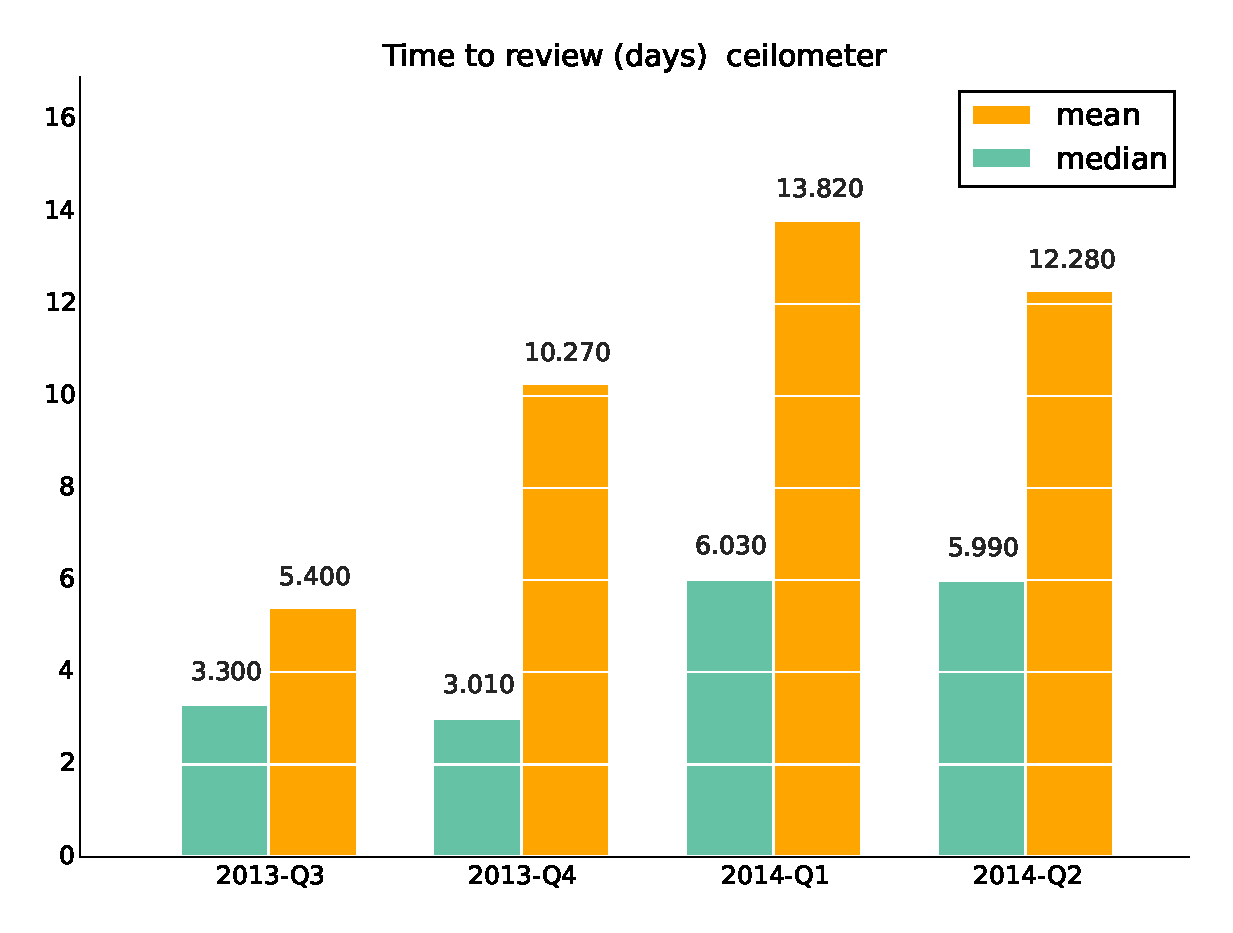
\includegraphics[scale=.35]{figs/timetoreview_medianceilometer.eps}
    & 
    \vspace{0pt}
    \begin{tabular}{l|r|r|}%
    \bfseries Period & \bfseries Median & \bfseries Mean % specify table head
    \csvreader[head to column names]{data/timetoreview_medianceilometer.csv}{}% use head of csv as column names
    {\\\labels & \mediantime & \meantime}
    \end{tabular}
\end{tabular}


 \newpage 
 \subsubsection{Cinder}

\textbf{Activity}: Commits in Git, submitted, merged and abandoned reviews in Gerrit and opened and closed issues in Launchpad.

\begin{tabular}{p{7cm} p{5cm}}
    \vspace{0pt} 
    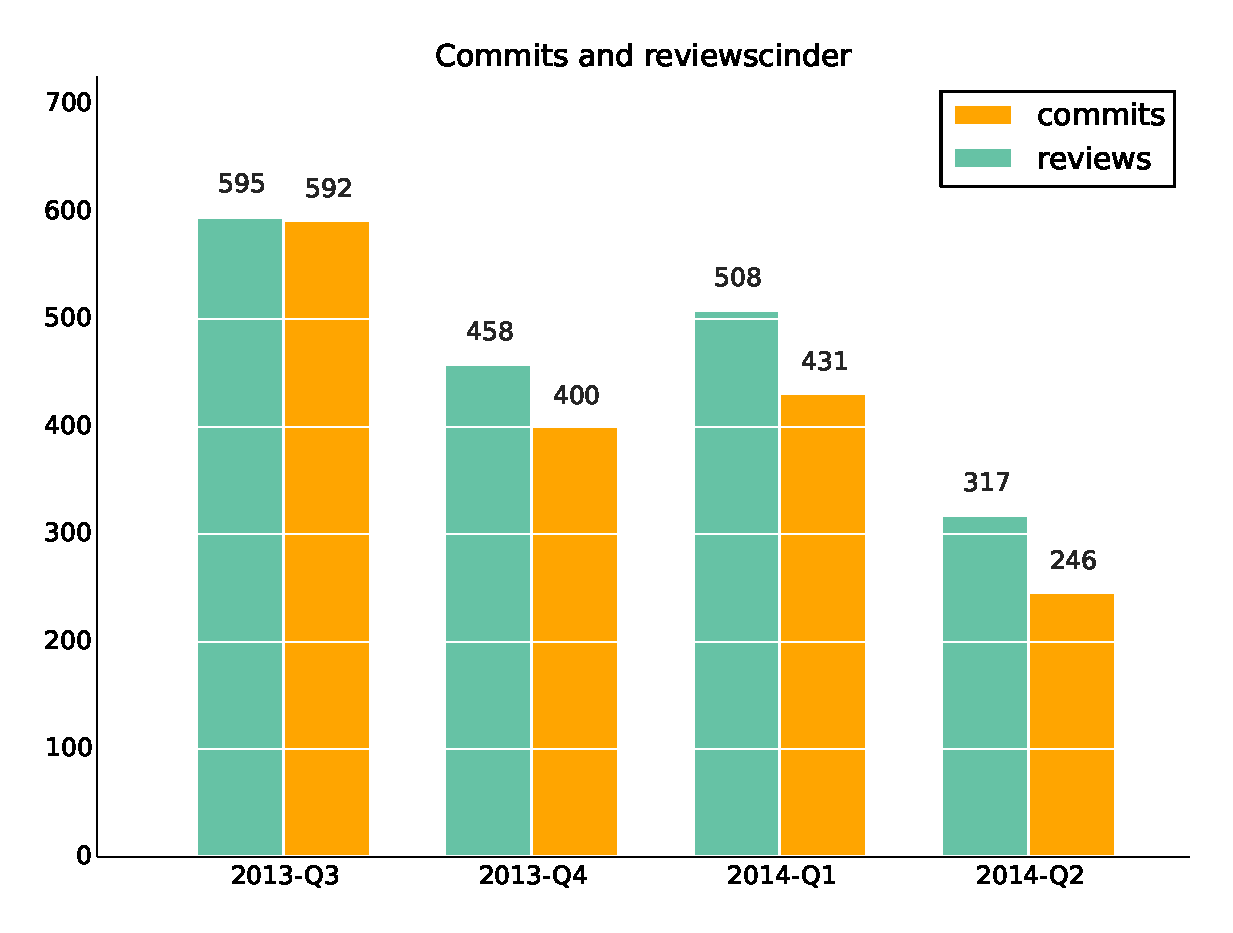
\includegraphics[scale=.35]{figs/commitscinder.eps}
    & 
    \vspace{0pt}
    \begin{tabular}{l|r|r|}%
    \bfseries Period & \bfseries Commits & \bfseries Reviews % specify table head
    \csvreader[head to column names]{data/commitscinder.csv}{}% use head of csv as column names
    {\\\labels & \commits & \submitted}
    \end{tabular}
\end{tabular}

\begin{tabular}{p{7cm} p{5cm}}
    \vspace{0pt} 
    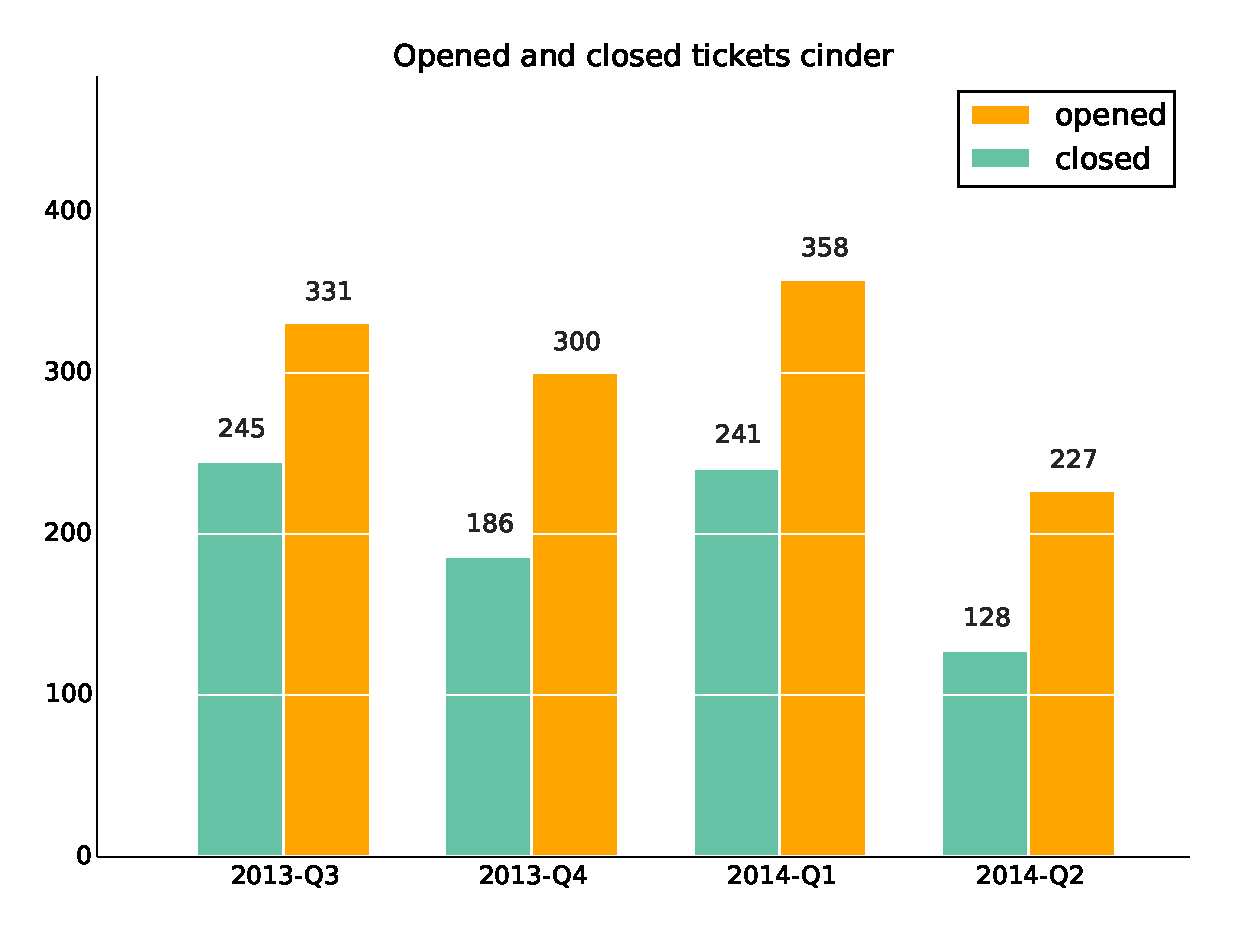
\includegraphics[scale=.35]{figs/closedcinder.eps}
    & 
    \vspace{0pt}
    \begin{tabular}{l|r|r|}%
    \bfseries Period & \bfseries Closed & \bfseries Opened
    \csvreader[head to column names]{data/closedcinder.csv}{}% use head of csv as column names
    {\\\labels & \closed & \opened}
    \end{tabular}
\end{tabular}

\begin{tabular}{p{7cm} p{5cm}}
    \vspace{0pt} 
    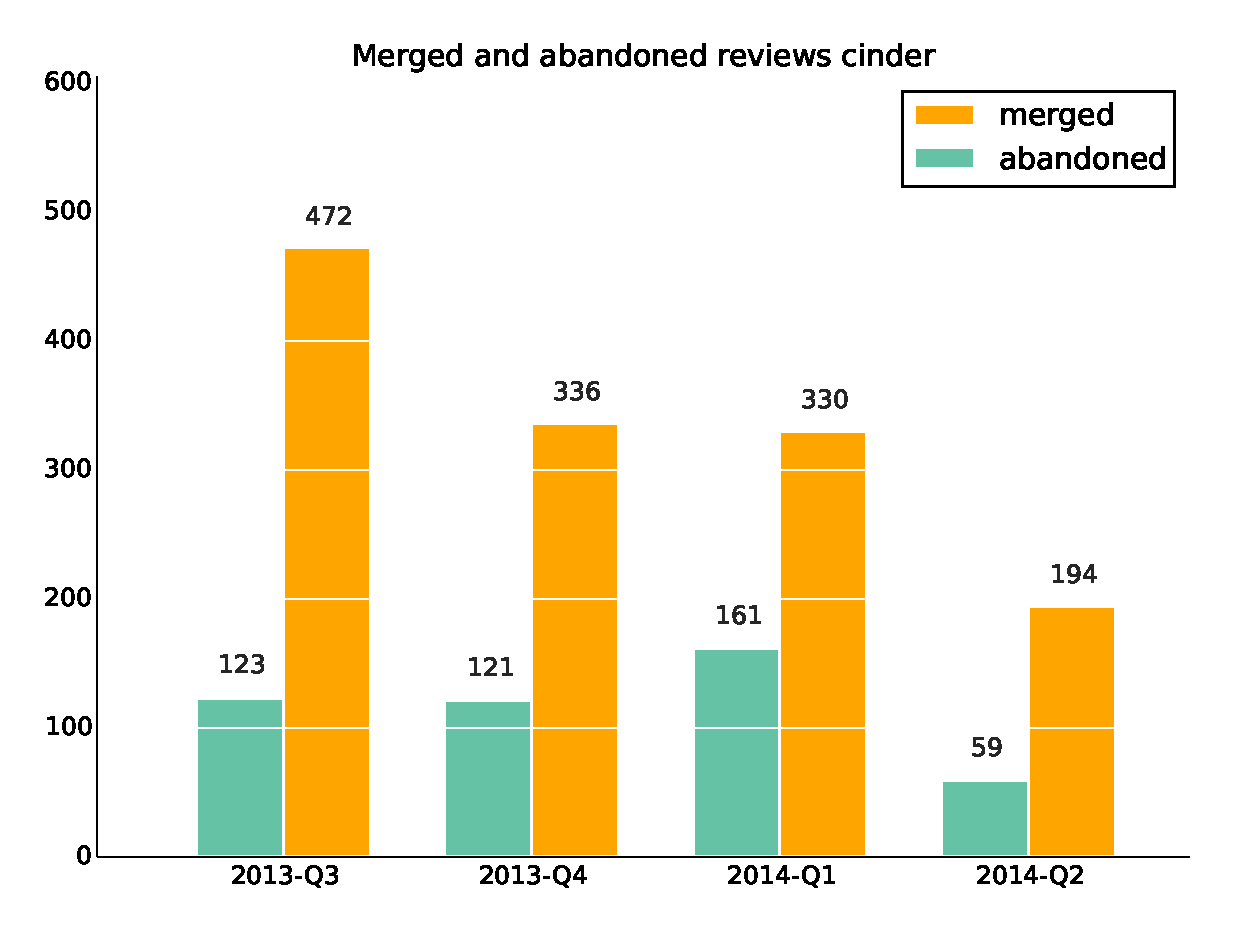
\includegraphics[scale=.35]{figs/submitted_reviewscinder.eps}
    & 
    \vspace{0pt}
    \begin{tabular}{l|r|r|}%
    \bfseries Period & \bfseries Merged & \bfseries Abandoned % specify table head
    \csvreader[head to column names]{data/submitted_reviewscinder.csv}{}% use head of csv as column names
    {\\\labels & \merged & \abandoned}
    \end{tabular}
\end{tabular}


\textbf{Community}: Authors per quarter and top authors and organizations in the last quarter

\begin{tabular}{p{7cm} p{5cm}}
    \vspace{0pt} 
    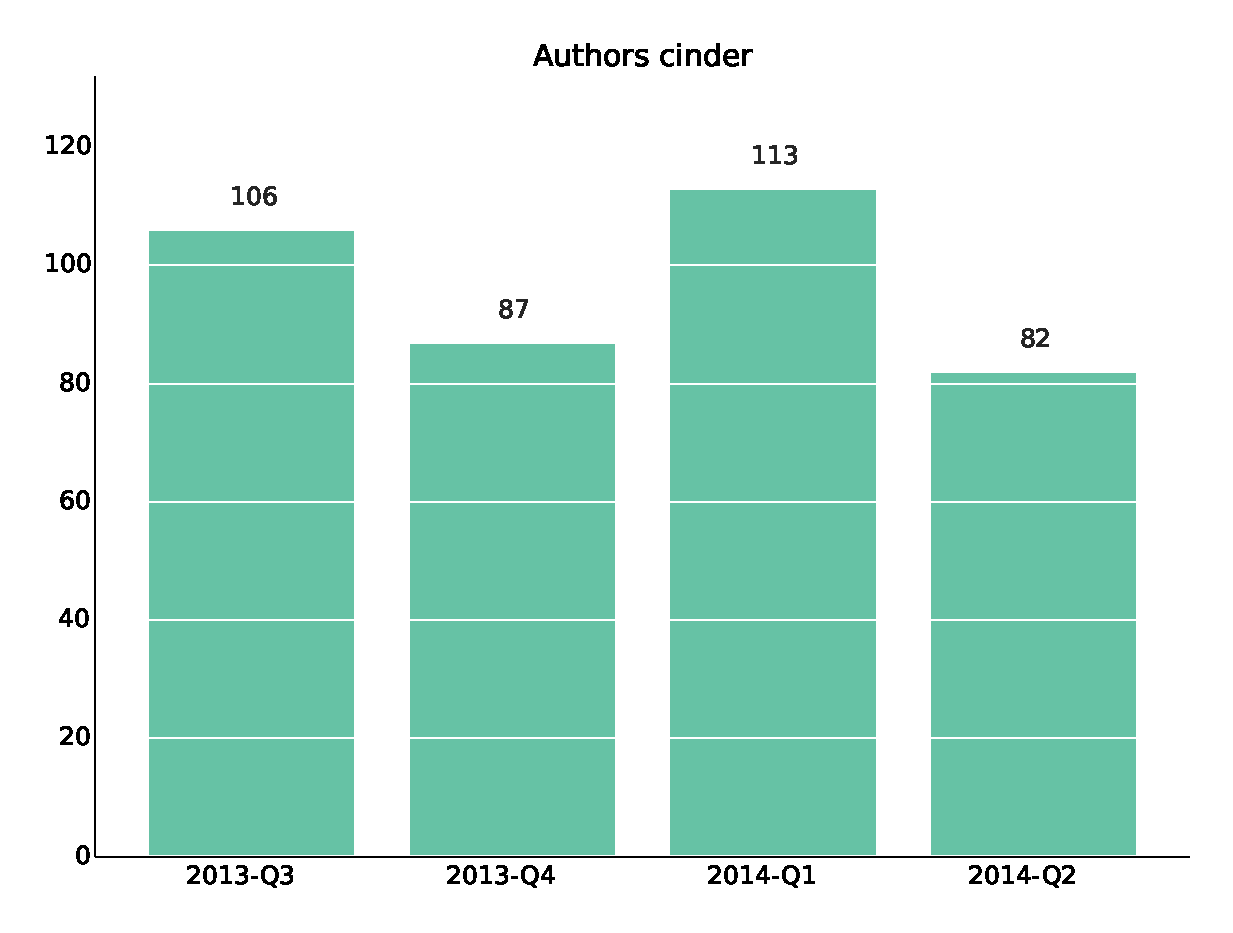
\includegraphics[scale=.35]{figs/authorscinder.eps}
    & 
    \vspace{0pt}
    \begin{tabular}{l|l}%
    \bfseries Period & \bfseries Authors % specify table head
    \csvreader[head to column names]{data/authorscinder.csv}{}% use head of csv as column names
    {\\\labels & \authors}
    \end{tabular}
\end{tabular}

\begin{tabular}{p{7cm} p{5cm}}
    \vspace{0pt}
\begin{tabular}{l|l}%
    \bfseries Commit (s) & \bfseries Author % specify table head
    \csvreader[head to column names]{data/scm_top_authors_project_cinder.csv}{}% use head of csv as column names
    {\\\hline\csvcoli&\csvcolii}% specify your coloumns here
\end{tabular}
&
\vspace{0pt}
\begin{tabular}{l|l}%
    \bfseries Commit (s) & \bfseries Organizations % specify table head
    \csvreader[head to column names]{data/scm_top_companies_project_cinder.csv}{}% use head of csv as column names
    {\\\hline\csvcoli&\csvcolii}% specify your coloumns here
\end{tabular}
\end {tabular}

\textbf{Process}: Efficiency closing issues and time to review: mean and median

\begin{tabular}{p{7cm} p{5cm}}
    \vspace{0pt} 
    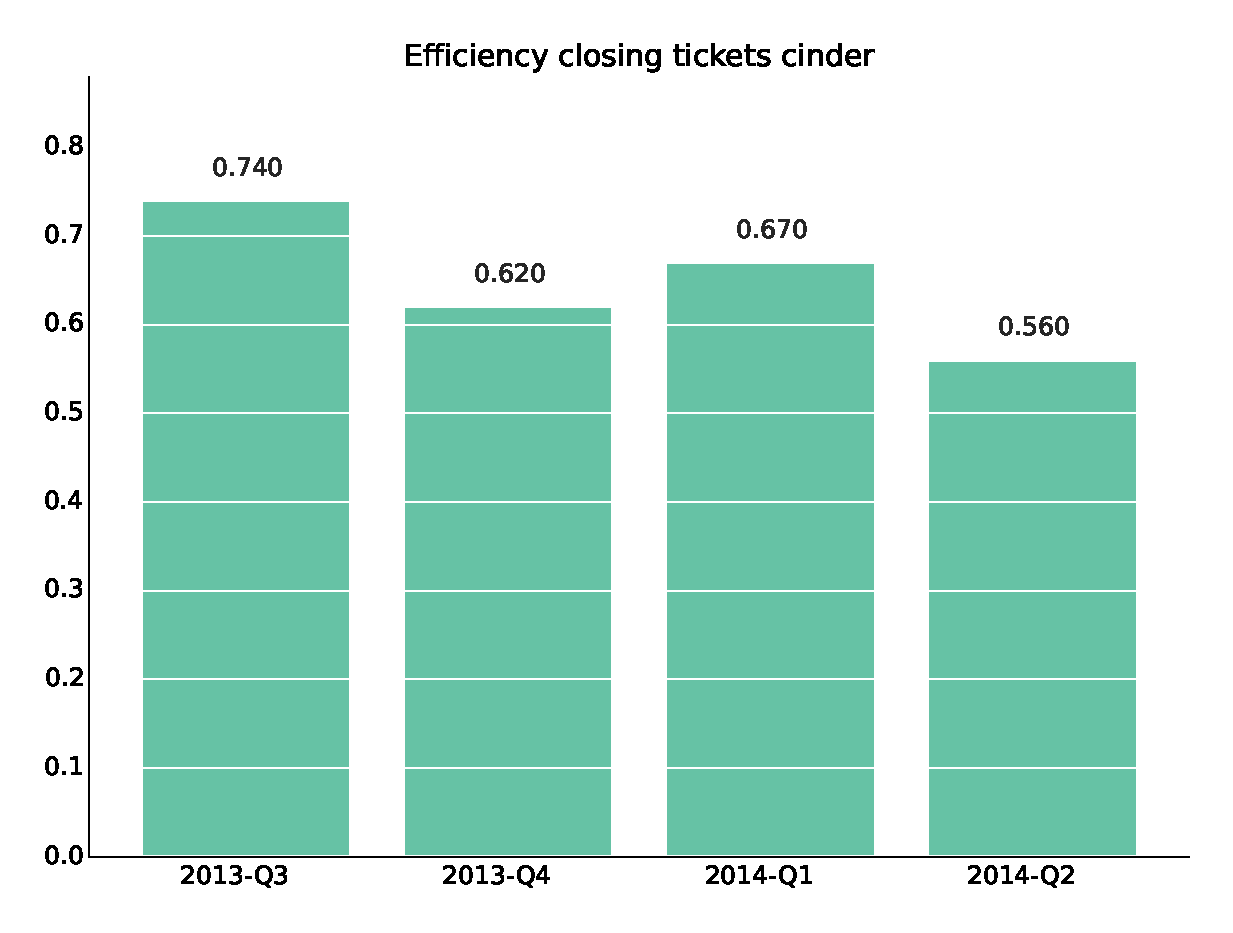
\includegraphics[scale=.35]{figs/bmicinder.eps}
    & 
    \vspace{0pt}
    \begin{tabular}{l|l}%
    \bfseries Period & \bfseries Closed/Opened % specify table head
    \csvreader[head to column names]{data/bmicinder.csv}{}% use head of csv as column names
    {\\\labels & \bmi}
    \end{tabular}
\end{tabular}

\begin{tabular}{p{7cm} p{5cm}}
    \vspace{0pt} 
    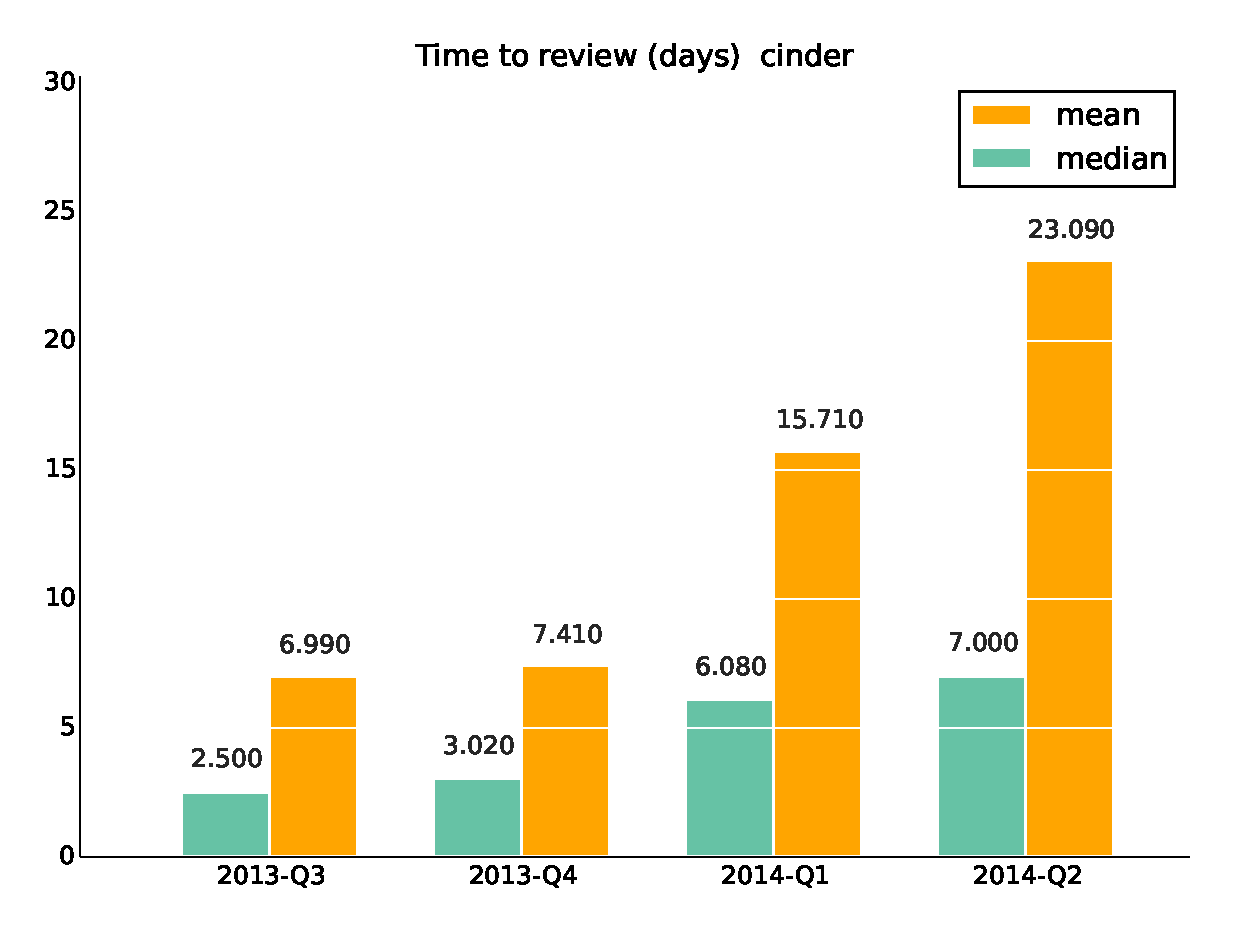
\includegraphics[scale=.35]{figs/timetoreview_mediancinder.eps}
    & 
    \vspace{0pt}
    \begin{tabular}{l|r|r|}%
    \bfseries Period & \bfseries Median & \bfseries Mean % specify table head
    \csvreader[head to column names]{data/timetoreview_mediancinder.csv}{}% use head of csv as column names
    {\\\labels & \mediantime & \meantime}
    \end{tabular}
\end{tabular}


 \newpage 
 \subsubsection{Glance}

\textbf{Activity}: Commits in Git, submitted, merged and abandoned reviews in Gerrit and opened and closed issues in Launchpad.

\begin{tabular}{p{7cm} p{5cm}}
    \vspace{0pt} 
    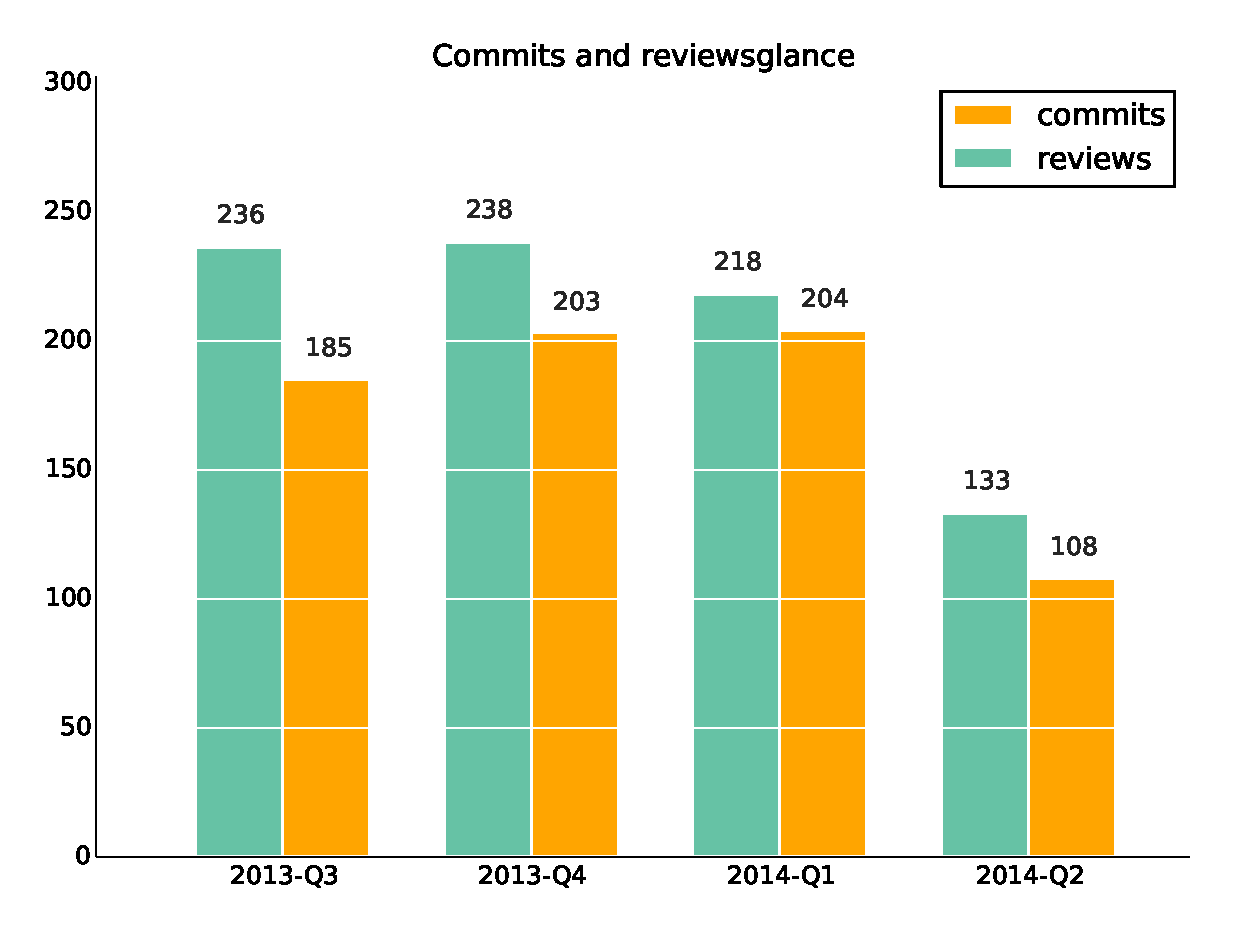
\includegraphics[scale=.35]{figs/commitsglance.eps}
    & 
    \vspace{0pt}
    \begin{tabular}{l|r|r|}%
    \bfseries Period & \bfseries Commits & \bfseries Reviews % specify table head
    \csvreader[head to column names]{data/commitsglance.csv}{}% use head of csv as column names
    {\\\labels & \commits & \submitted}
    \end{tabular}
\end{tabular}

\begin{tabular}{p{7cm} p{5cm}}
    \vspace{0pt} 
    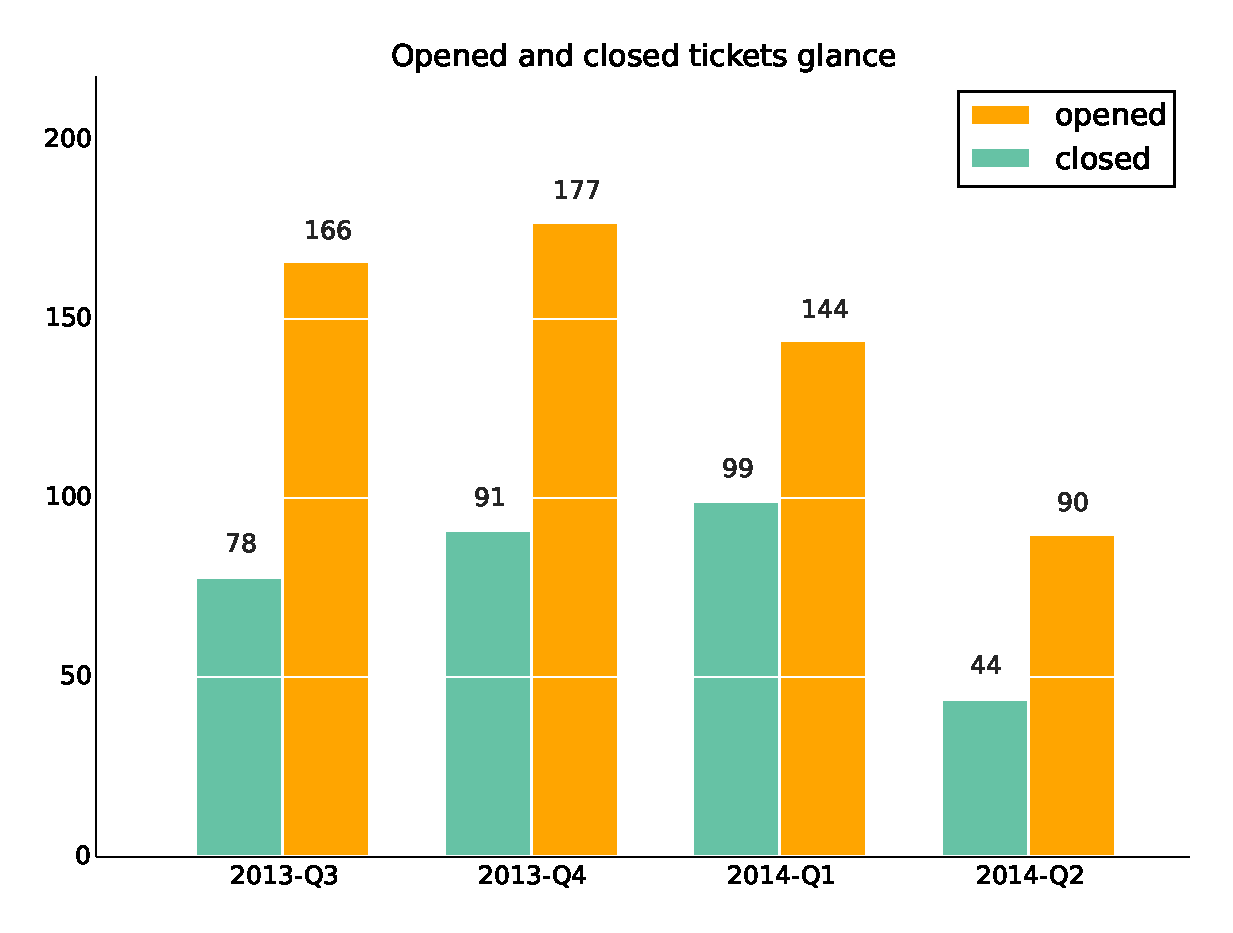
\includegraphics[scale=.35]{figs/closedglance.eps}
    & 
    \vspace{0pt}
    \begin{tabular}{l|r|r|}%
\bfseries Period & \bfseries Closed & \bfseries Opened
    \csvreader[head to column names]{data/closedglance.csv}{}% use head of csv as column names
    {\\\labels & \closed & \opened}
    \end{tabular}
\end{tabular}

\begin{tabular}{p{7cm} p{5cm}}
    \vspace{0pt} 
    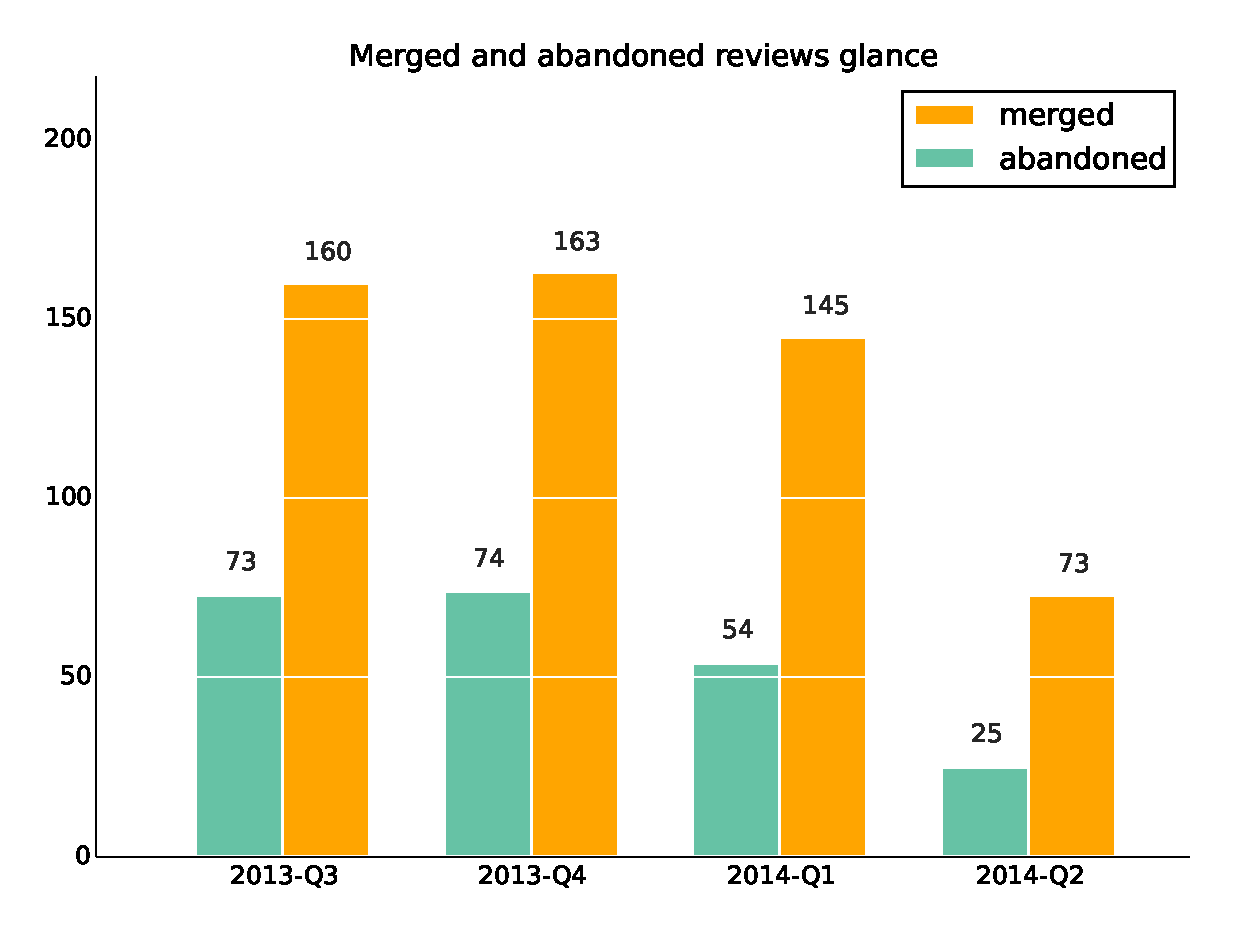
\includegraphics[scale=.35]{figs/submitted_reviewsglance.eps}
    & 
    \vspace{0pt}
    \begin{tabular}{l|r|r|}%
    \bfseries Period & \bfseries Merged & \bfseries Abandoned % specify table head
    \csvreader[head to column names]{data/submitted_reviewsglance.csv}{}% use head of csv as column names
    {\\\labels & \merged & \abandoned}
    \end{tabular}
\end{tabular}


\textbf{Community}: Authors per quarter and top authors and organizations in the last quarter

\begin{tabular}{p{7cm} p{5cm}}
    \vspace{0pt} 
    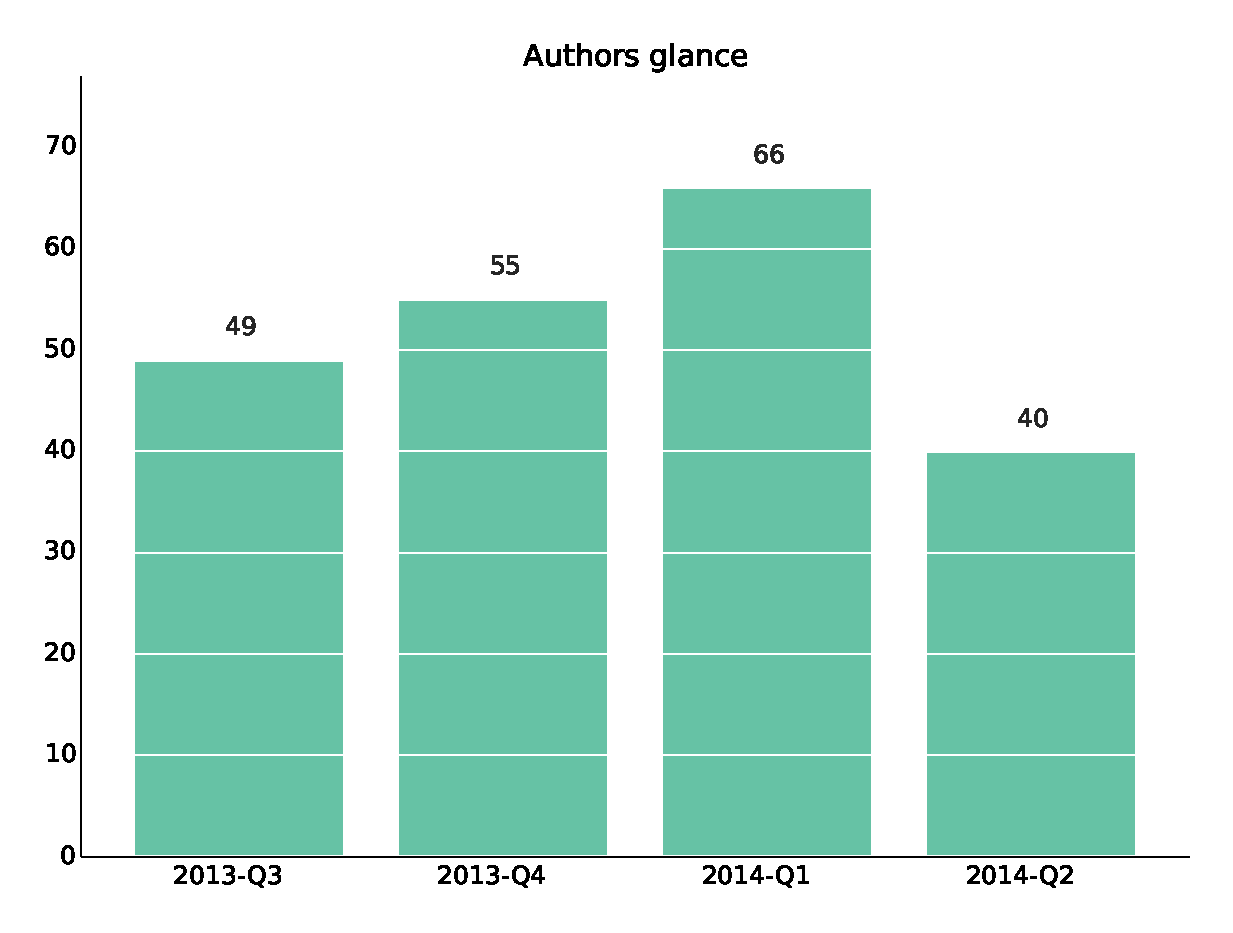
\includegraphics[scale=.35]{figs/authorsglance.eps}
    & 
    \vspace{0pt}
    \begin{tabular}{l|l}%
    \bfseries Period & \bfseries Authors % specify table head
    \csvreader[head to column names]{data/authorsglance.csv}{}% use head of csv as column names
    {\\\labels & \authors}
    \end{tabular}
\end{tabular}

\begin{tabular}{p{7cm} p{5cm}}
    \vspace{0pt}
\begin{tabular}{l|l}%
    \bfseries Commit (s) & \bfseries Author % specify table head
    \csvreader[head to column names]{data/scm_top_authors_project_glance.csv}{}% use head of csv as column names
    {\\\hline\csvcoli&\csvcolii}% specify your coloumns here
\end{tabular}
&
\vspace{0pt}
\begin{tabular}{l|l}%
    \bfseries Commit (s) & \bfseries Organizations % specify table head
    \csvreader[head to column names]{data/scm_top_companies_project_glance.csv}{}% use head of csv as column names
    {\\\hline\csvcoli&\csvcolii}% specify your coloumns here
\end{tabular}
\end {tabular}

\textbf{Process}: Efficiency closing issues and time to review: mean and median

\begin{tabular}{p{7cm} p{5cm}}
    \vspace{0pt} 
    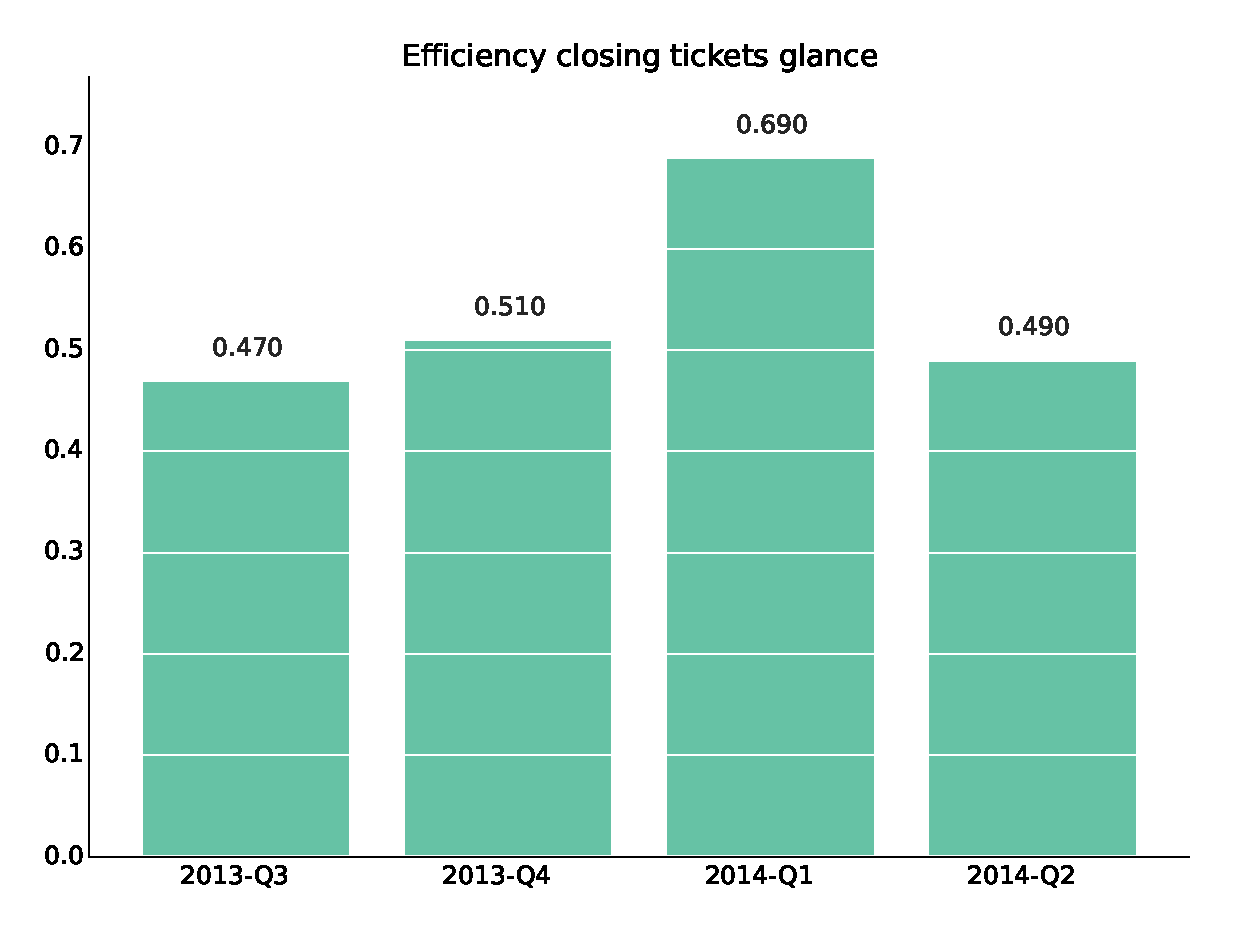
\includegraphics[scale=.35]{figs/bmiglance.eps}
    & 
    \vspace{0pt}
    \begin{tabular}{l|l}%
    \bfseries Period & \bfseries Closed/Opened % specify table head
    \csvreader[head to column names]{data/bmiglance.csv}{}% use head of csv as column names
    {\\\labels & \bmi}
    \end{tabular}
\end{tabular}

\begin{tabular}{p{7cm} p{5cm}}
    \vspace{0pt} 
    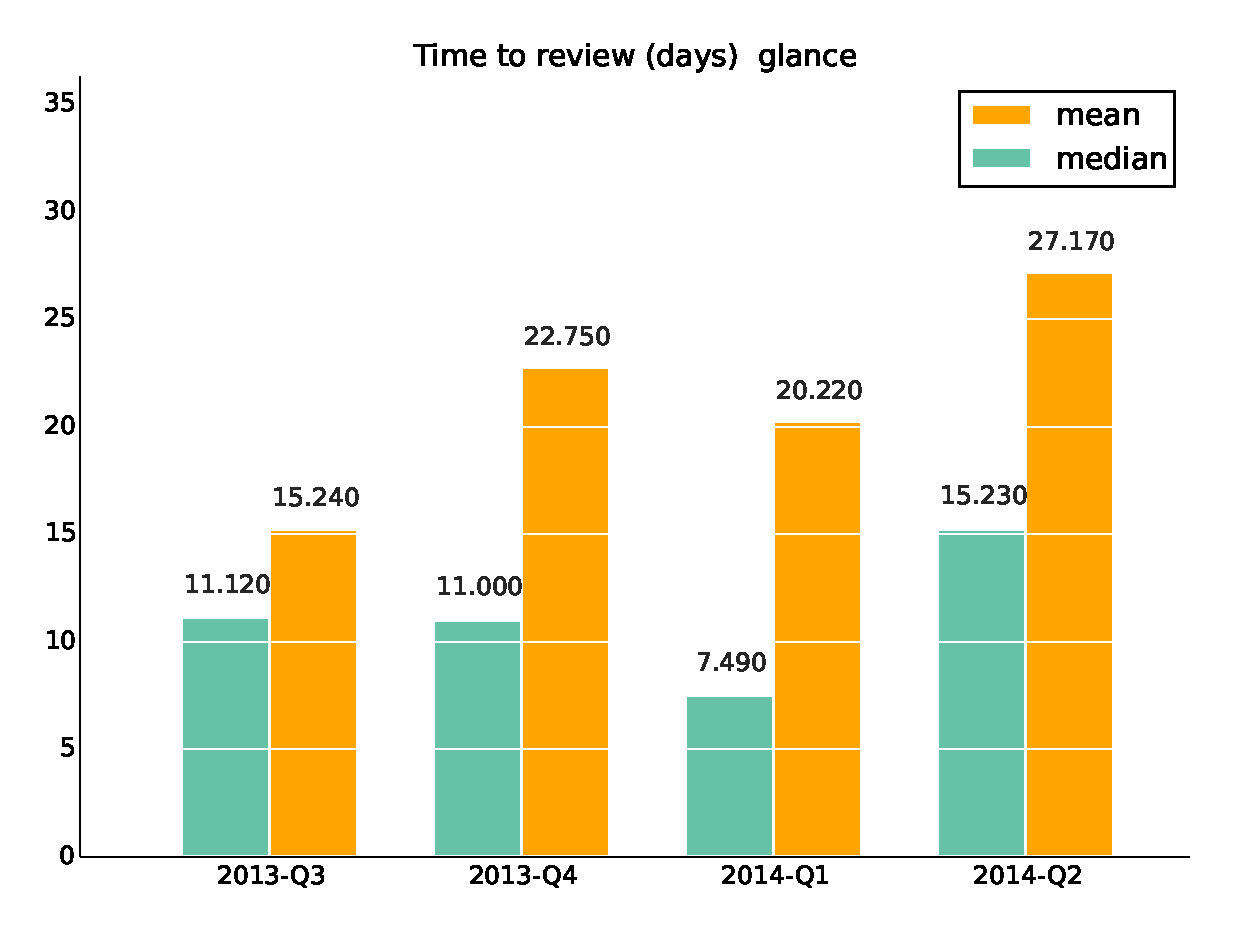
\includegraphics[scale=.35]{figs/timetoreview_medianglance.eps}
    & 
    \vspace{0pt}
    \begin{tabular}{l|r|r|}%
    \bfseries Period & \bfseries Median & \bfseries Mean % specify table head
    \csvreader[head to column names]{data/timetoreview_medianglance.csv}{}% use head of csv as column names
    {\\\labels & \mediantime & \meantime}
    \end{tabular}
\end{tabular}


 \newpage 
 \subsubsection{Heat}

\textbf{Activity}: Commits in Git, submitted, merged and abandoned reviews in Gerrit and opened and closed issues in Launchpad.

\begin{tabular}{p{7cm} p{5cm}}
    \vspace{0pt} 
    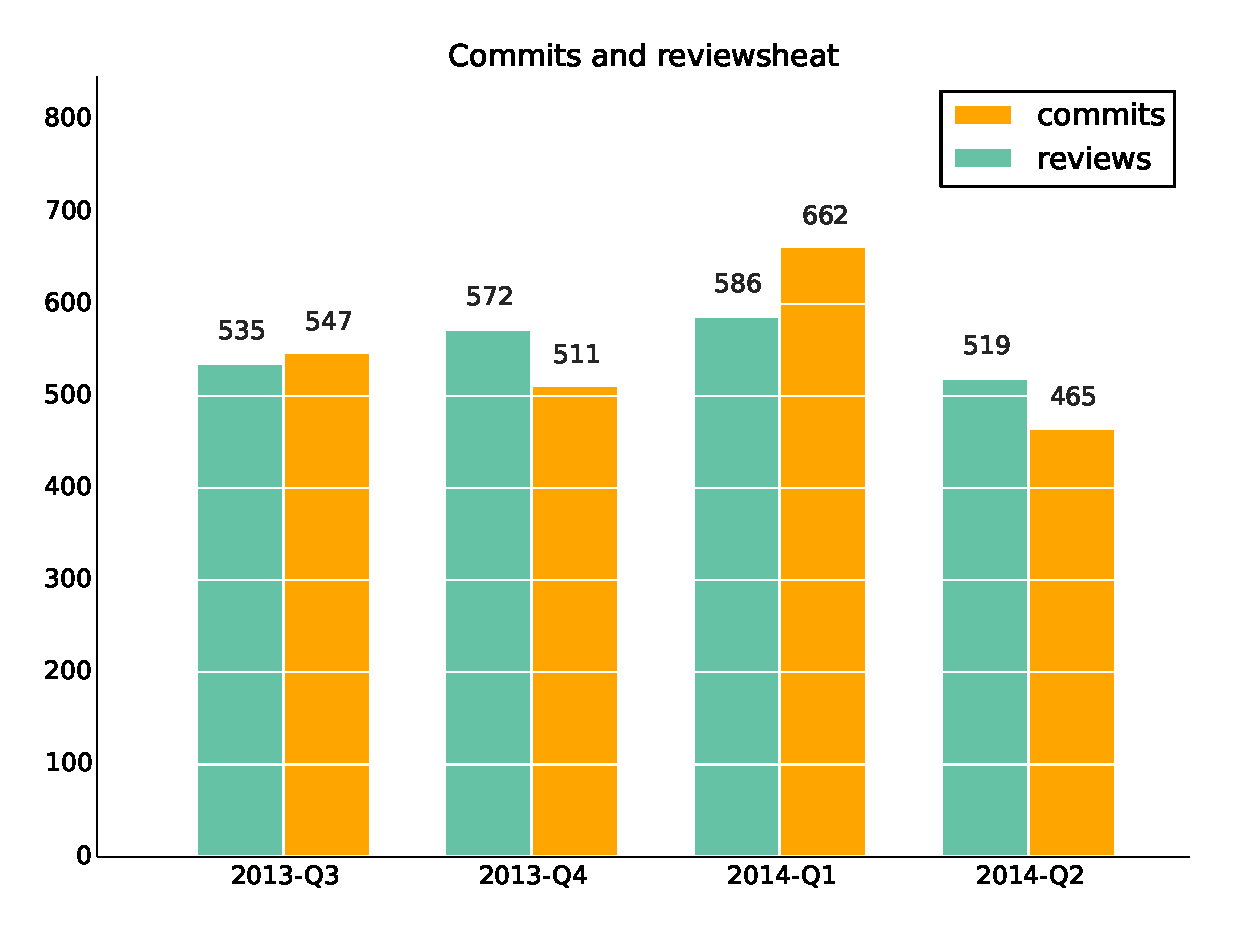
\includegraphics[scale=.35]{figs/commitsheat.eps}
    & 
    \vspace{0pt}
    \begin{tabular}{l|r|r|}%
    \bfseries Period & \bfseries Commits & \bfseries Reviews % specify table head
    \csvreader[head to column names]{data/commitsheat.csv}{}% use head of csv as column names
    {\\\labels & \commits & \submitted}
    \end{tabular}
\end{tabular}

\begin{tabular}{p{7cm} p{5cm}}
    \vspace{0pt} 
    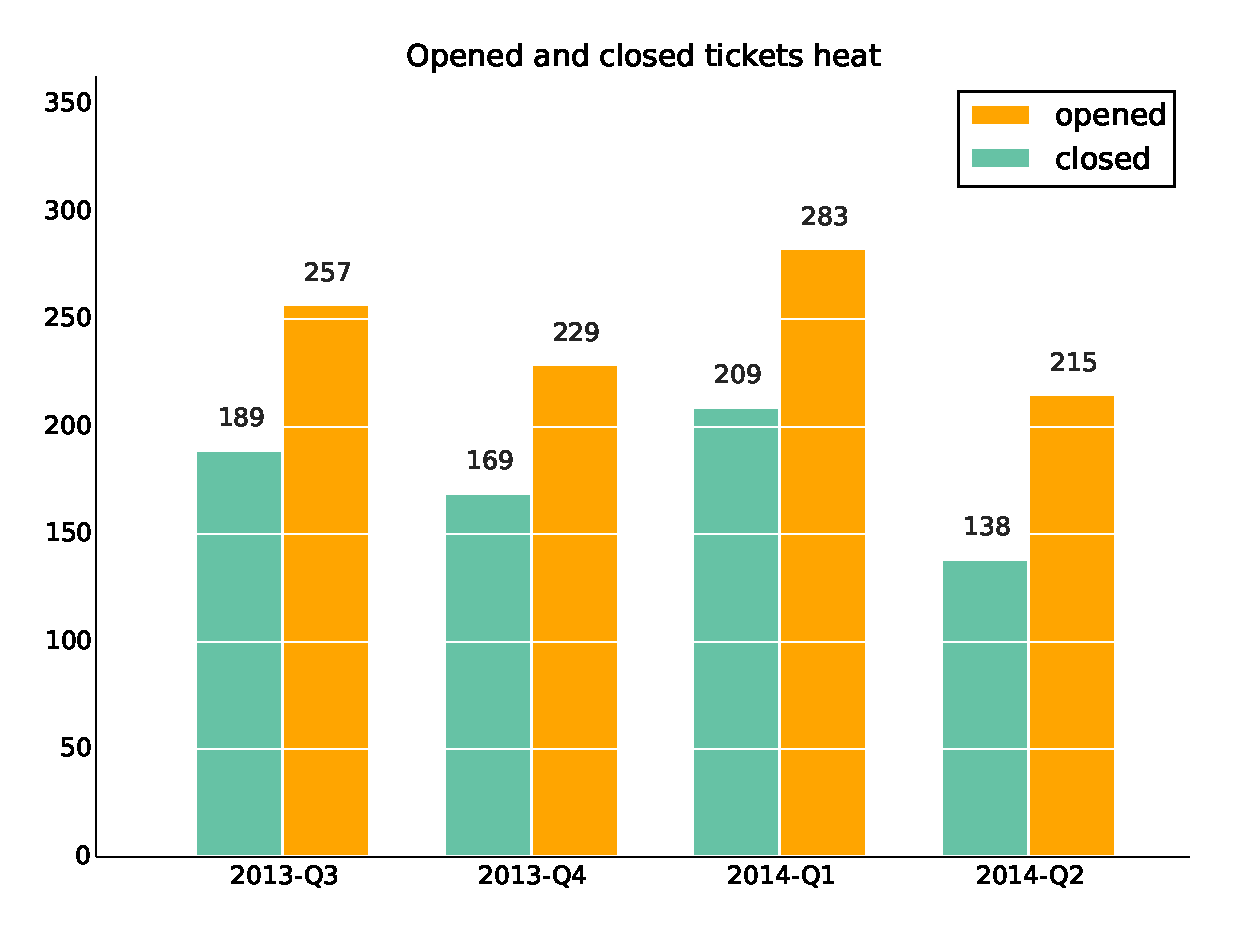
\includegraphics[scale=.35]{figs/closedheat.eps}
    & 
    \vspace{0pt}
    \begin{tabular}{l|r|r|}%
\bfseries Period & \bfseries Closed & \bfseries Opened
    \csvreader[head to column names]{data/closedheat.csv}{}% use head of csv as column names
    {\\\labels & \closed & \opened}
    \end{tabular}
\end{tabular}

\begin{tabular}{p{7cm} p{5cm}}
    \vspace{0pt} 
    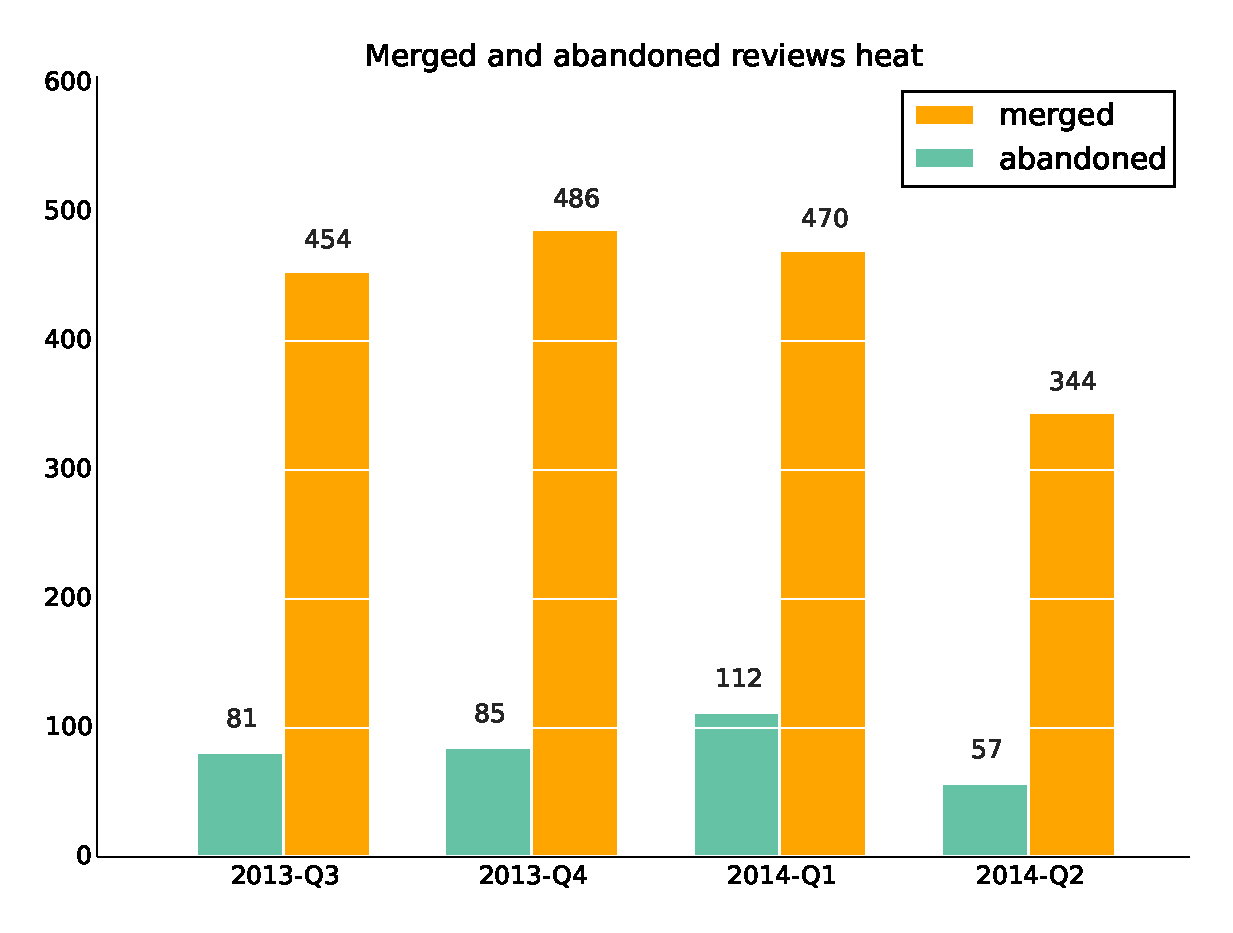
\includegraphics[scale=.35]{figs/submitted_reviewsheat.eps}
    & 
    \vspace{0pt}
    \begin{tabular}{l|r|r|}%
    \bfseries Period & \bfseries Merged & \bfseries Abandoned % specify table head
    \csvreader[head to column names]{data/submitted_reviewsheat.csv}{}% use head of csv as column names
    {\\\labels & \merged & \abandoned}
    \end{tabular}
\end{tabular}


\textbf{Community}: Authors per quarter and top authors and organizations in the last quarter

\begin{tabular}{p{7cm} p{5cm}}
    \vspace{0pt} 
    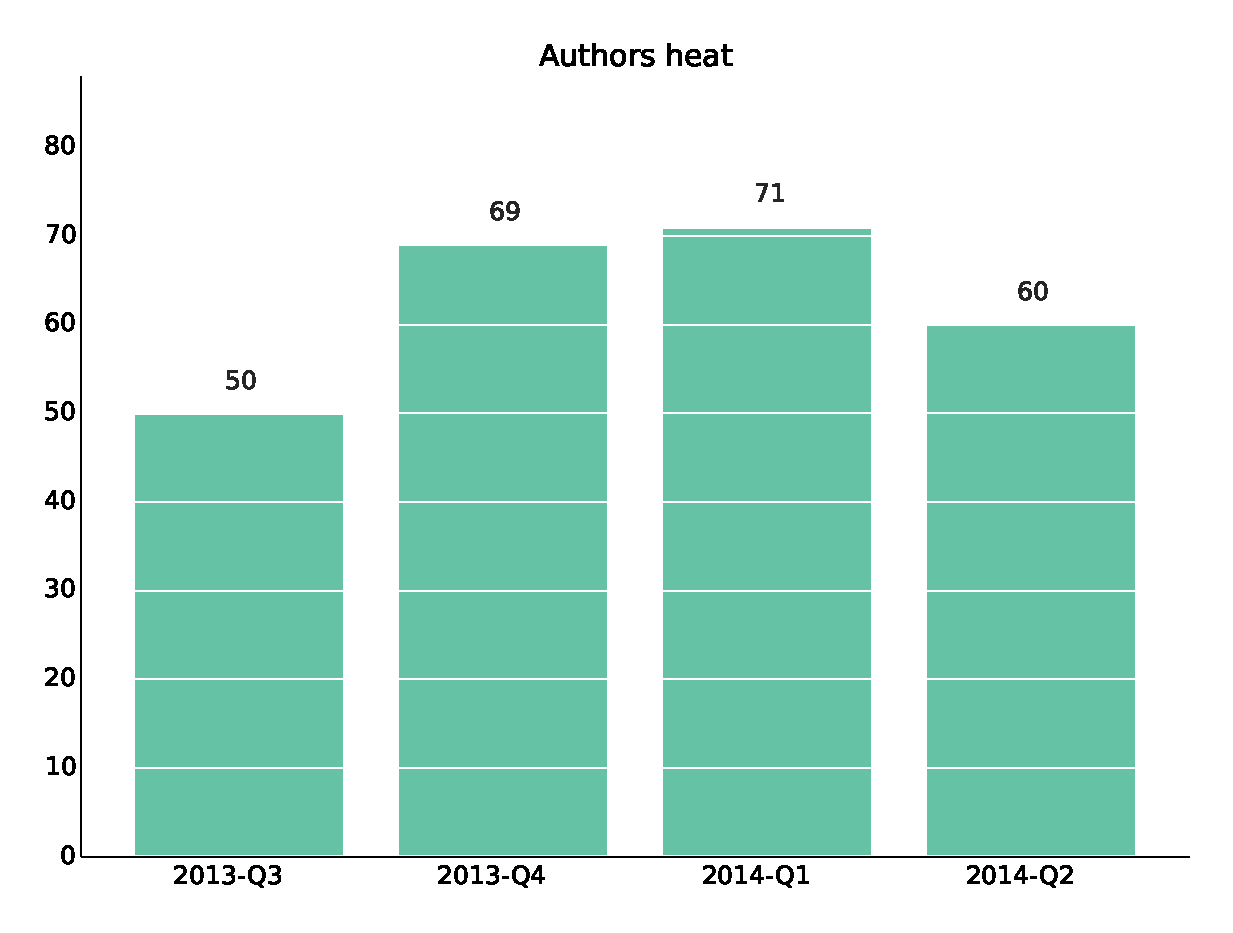
\includegraphics[scale=.35]{figs/authorsheat.eps}
    & 
    \vspace{0pt}
    \begin{tabular}{l|l}%
    \bfseries Period & \bfseries Authors % specify table head
    \csvreader[head to column names]{data/authorsheat.csv}{}% use head of csv as column names
    {\\\labels & \authors}
    \end{tabular}
\end{tabular}

\begin{tabular}{p{7cm} p{5cm}}
    \vspace{0pt}
\begin{tabular}{l|l}%
    \bfseries Commit (s) & \bfseries Author % specify table head
    \csvreader[head to column names]{data/scm_top_authors_project_heat.csv}{}% use head of csv as column names
    {\\\hline\csvcoli&\csvcolii}% specify your coloumns here
\end{tabular}
&
\vspace{0pt}
\begin{tabular}{l|l}%
    \bfseries Commit (s) & \bfseries Organizations % specify table head
    \csvreader[head to column names]{data/scm_top_companies_project_heat.csv}{}% use head of csv as column names
    {\\\hline\csvcoli&\csvcolii}% specify your coloumns here
\end{tabular}
\end {tabular}

\textbf{Process}: Efficiency closing issues and time to review: mean and median

\begin{tabular}{p{7cm} p{5cm}}
    \vspace{0pt} 
    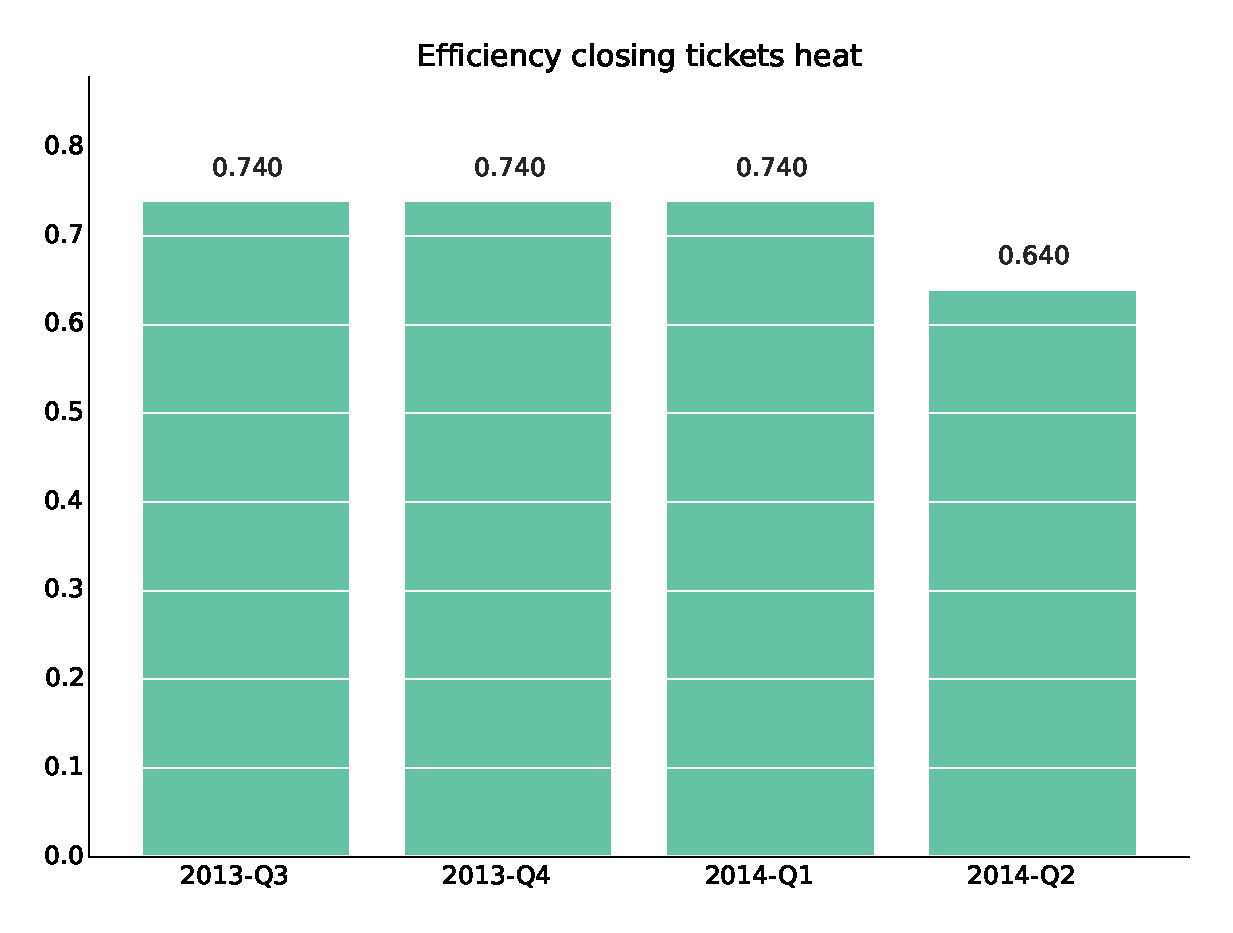
\includegraphics[scale=.35]{figs/bmiheat.eps}
    & 
    \vspace{0pt}
    \begin{tabular}{l|l}%
    \bfseries Period & \bfseries Closed/Opened % specify table head
    \csvreader[head to column names]{data/bmiheat.csv}{}% use head of csv as column names
    {\\\labels & \bmi}
    \end{tabular}
\end{tabular}

\begin{tabular}{p{7cm} p{5cm}}
    \vspace{0pt} 
    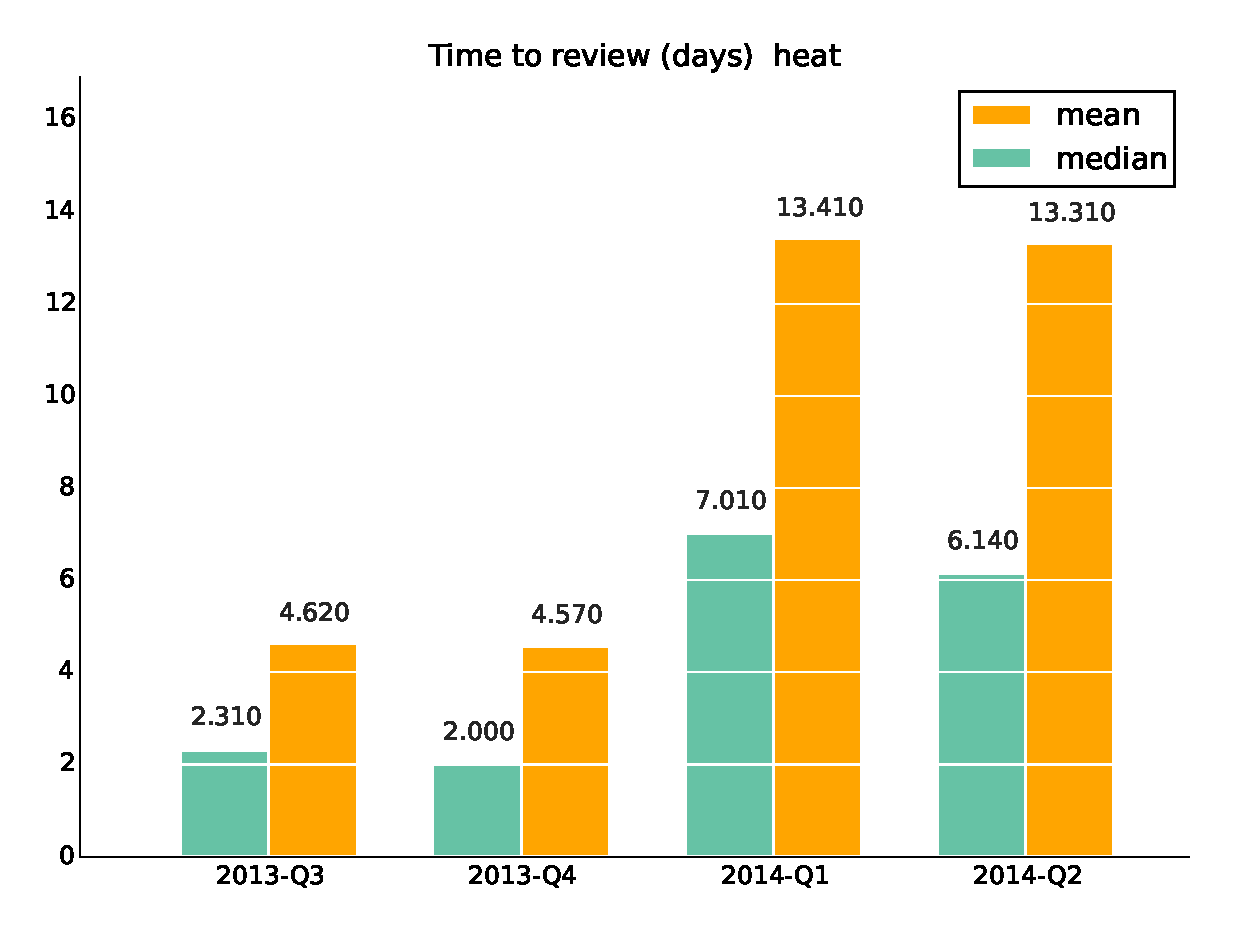
\includegraphics[scale=.35]{figs/timetoreview_medianheat.eps}
    & 
    \vspace{0pt}
    \begin{tabular}{l|r|r|}%
    \bfseries Period & \bfseries Median & \bfseries Mean % specify table head
    \csvreader[head to column names]{data/timetoreview_medianheat.csv}{}% use head of csv as column names
    {\\\labels & \mediantime & \meantime}
    \end{tabular}
\end{tabular}


 \newpage 
 \subsubsection{Horizon}

\textbf{Activity}: Commits in Git, submitted, merged and abandoned reviews in Gerrit and opened and closed issues in Launchpad.

\begin{tabular}{p{7cm} p{5cm}}
    \vspace{0pt} 
    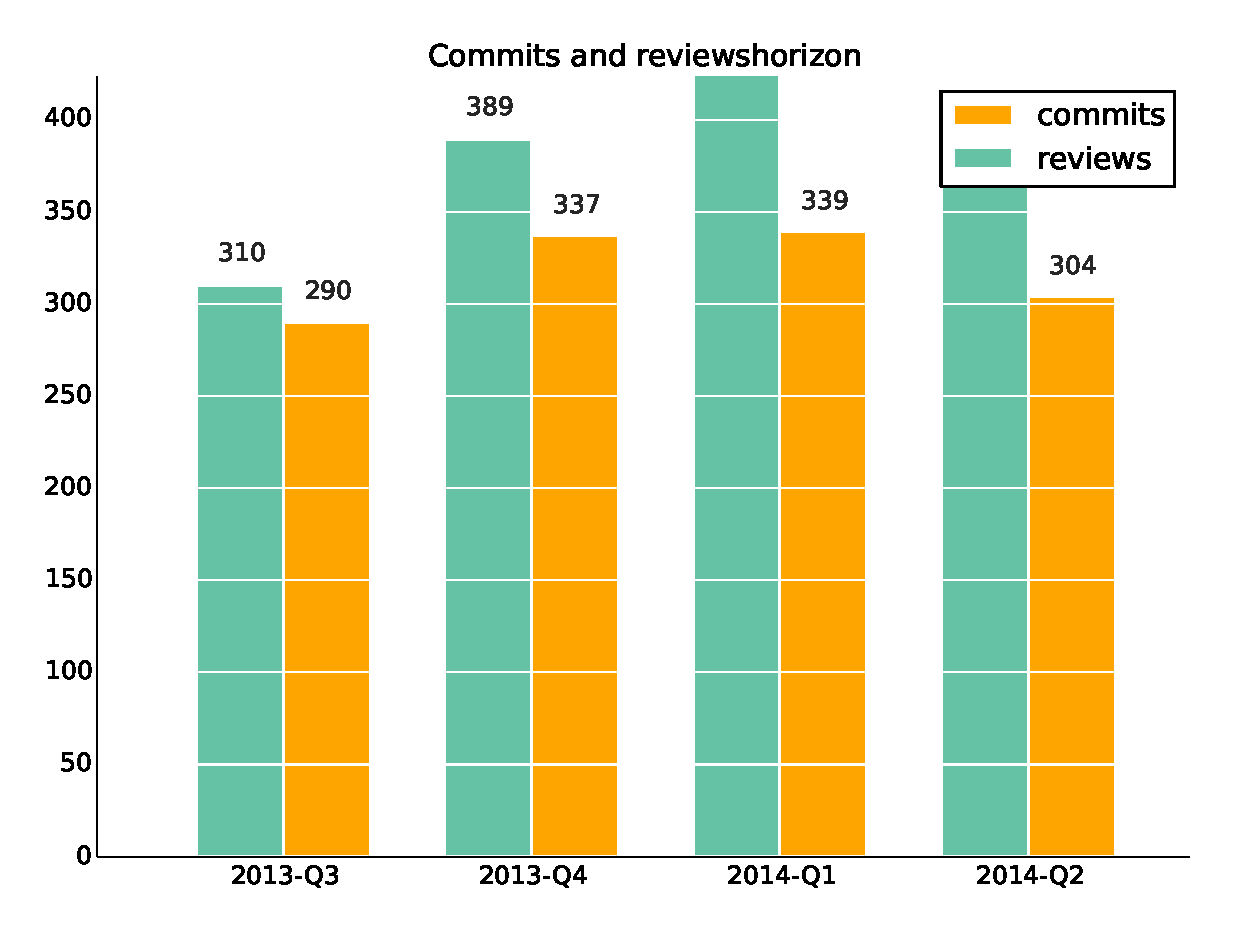
\includegraphics[scale=.35]{figs/commitshorizon.eps}
    & 
    \vspace{0pt}
    \begin{tabular}{l|r|r|}%
    \bfseries Period & \bfseries Commits & \bfseries Reviews % specify table head
    \csvreader[head to column names]{data/commitshorizon.csv}{}% use head of csv as column names
    {\\\labels & \commits & \submitted}
    \end{tabular}
\end{tabular}

\begin{tabular}{p{7cm} p{5cm}}
    \vspace{0pt} 
    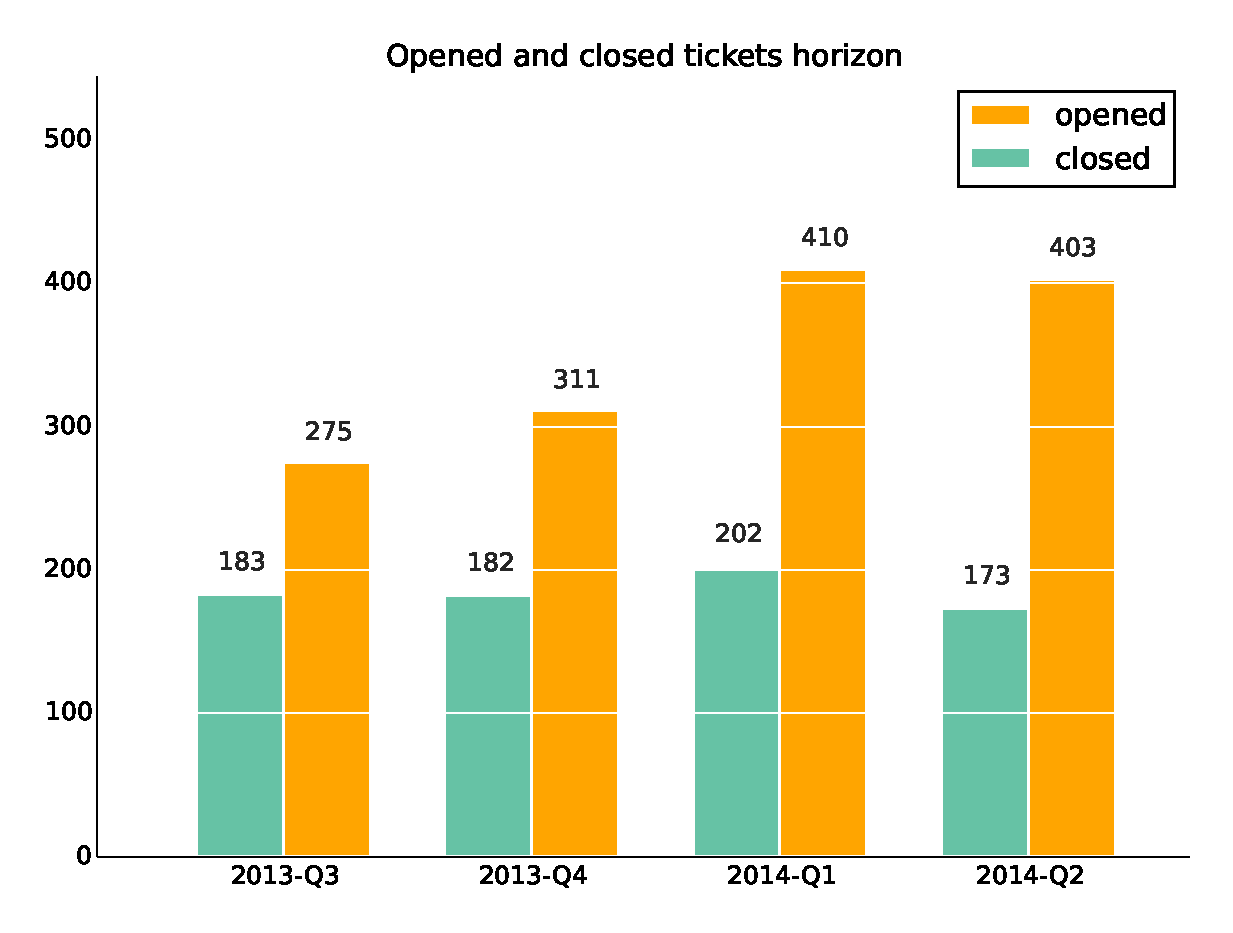
\includegraphics[scale=.35]{figs/closedhorizon.eps}
    & 
    \vspace{0pt}
    \begin{tabular}{l|r|r|}%
\bfseries Period & \bfseries Closed & \bfseries Opened
    \csvreader[head to column names]{data/closedhorizon.csv}{}% use head of csv as column names
    {\\\labels & \closed & \opened}
    \end{tabular}
\end{tabular}

\begin{tabular}{p{7cm} p{5cm}}
    \vspace{0pt} 
    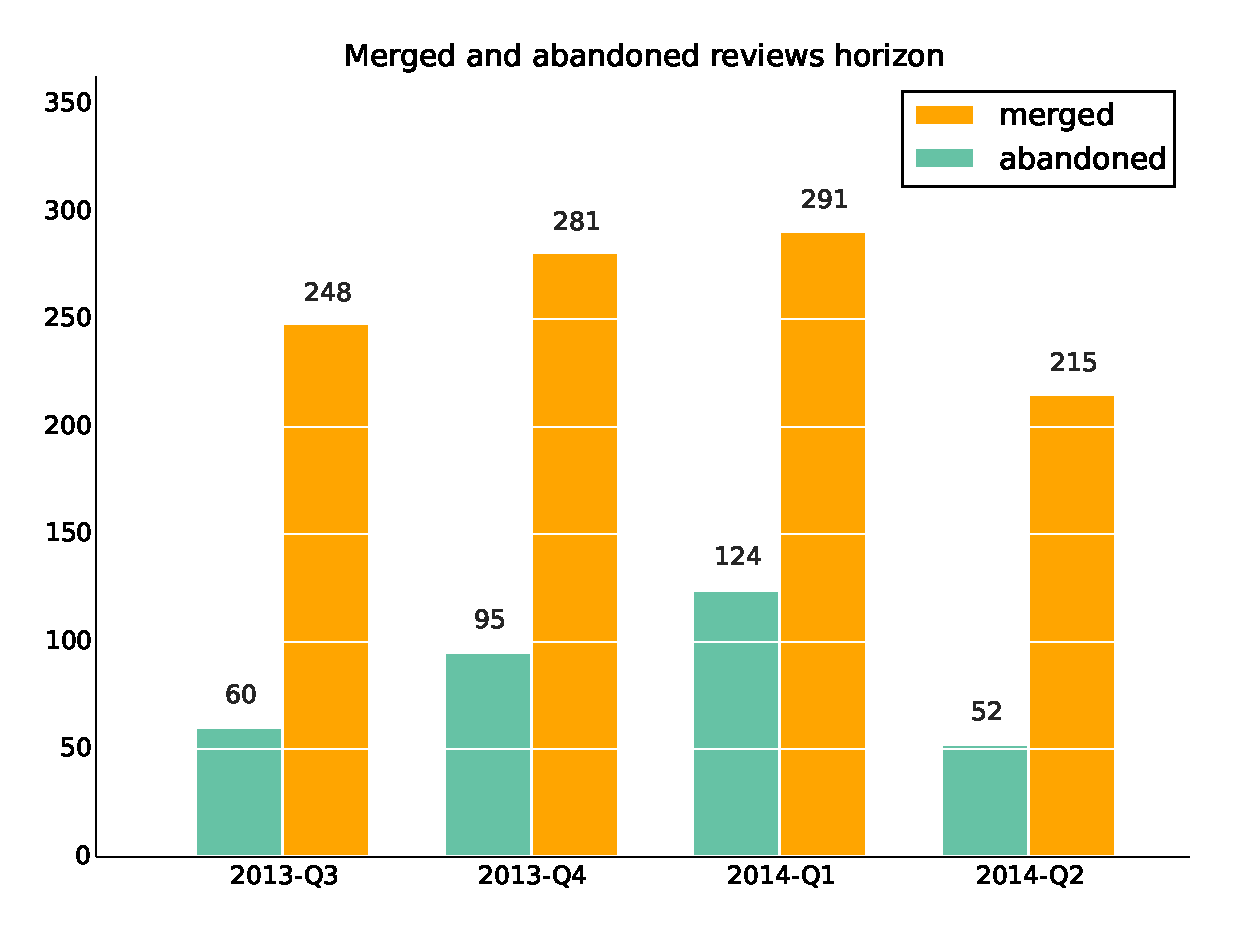
\includegraphics[scale=.35]{figs/submitted_reviewshorizon.eps}
    & 
    \vspace{0pt}
    \begin{tabular}{l|r|r|}%
    \bfseries Period & \bfseries Merged & \bfseries Abandoned % specify table head
    \csvreader[head to column names]{data/submitted_reviewshorizon.csv}{}% use head of csv as column names
    {\\\labels & \merged & \abandoned}
    \end{tabular}
\end{tabular}


\textbf{Community}: Authors per quarter and top authors and organizations in the last quarter

\begin{tabular}{p{7cm} p{5cm}}
    \vspace{0pt} 
    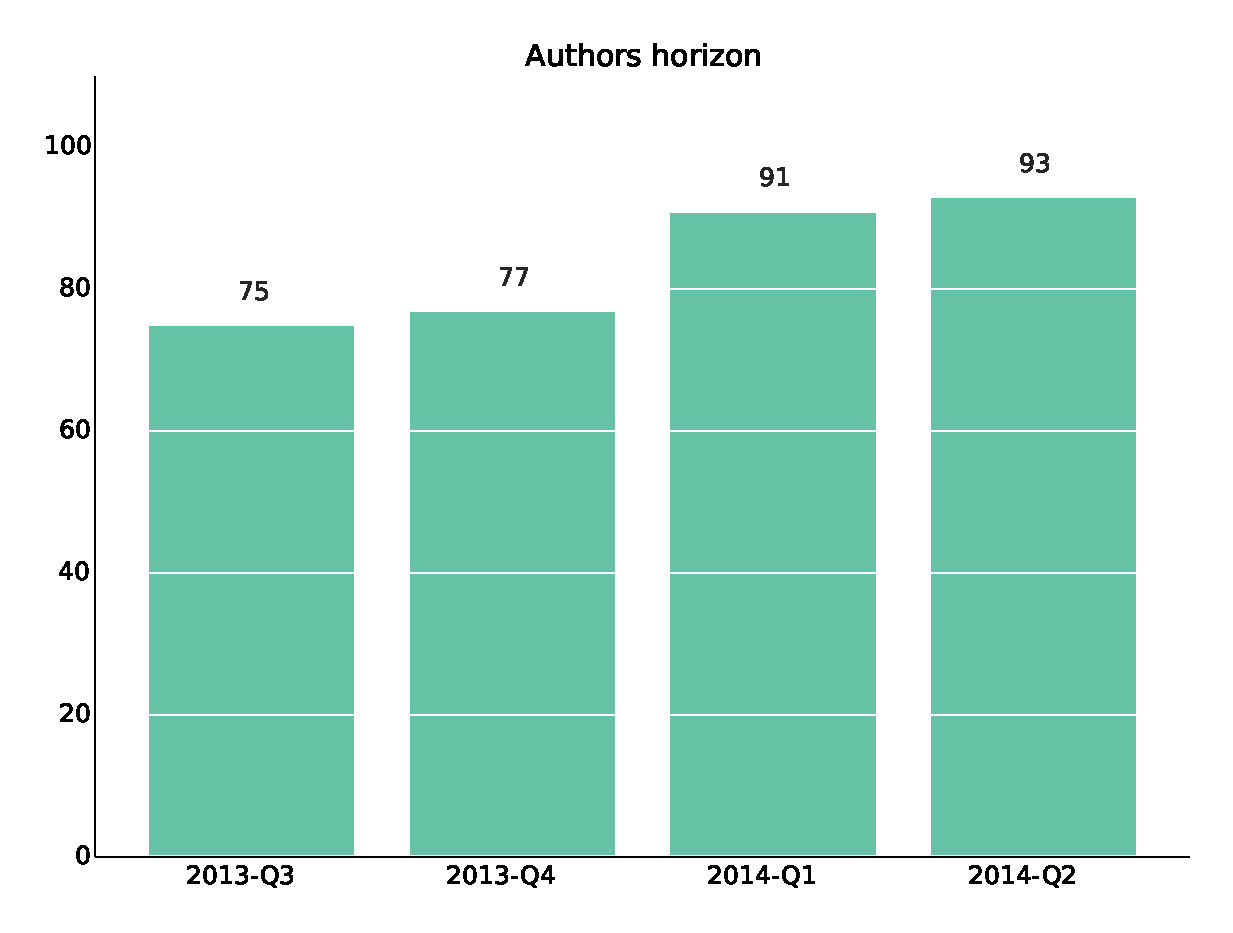
\includegraphics[scale=.35]{figs/authorshorizon.eps}
    & 
    \vspace{0pt}
    \begin{tabular}{l|l}%
    \bfseries Period & \bfseries Authors % specify table head
    \csvreader[head to column names]{data/authorshorizon.csv}{}% use head of csv as column names
    {\\\labels & \authors}
    \end{tabular}
\end{tabular}

\begin{tabular}{p{7cm} p{5cm}}
    \vspace{0pt}
\begin{tabular}{l|l}%
    \bfseries Commit (s) & \bfseries Author % specify table head
    \csvreader[head to column names]{data/scm_top_authors_project_horizon.csv}{}% use head of csv as column names
    {\\\hline\csvcoli&\csvcolii}% specify your coloumns here
\end{tabular}
&
\vspace{0pt}
\begin{tabular}{l|l}%
    \bfseries Commit (s) & \bfseries Organizations % specify table head
    \csvreader[head to column names]{data/scm_top_companies_project_horizon.csv}{}% use head of csv as column names
    {\\\hline\csvcoli&\csvcolii}% specify your coloumns here
\end{tabular}
\end {tabular}

\textbf{Process}: Efficiency closing issues and time to review: mean and median

\begin{tabular}{p{7cm} p{5cm}}
    \vspace{0pt} 
    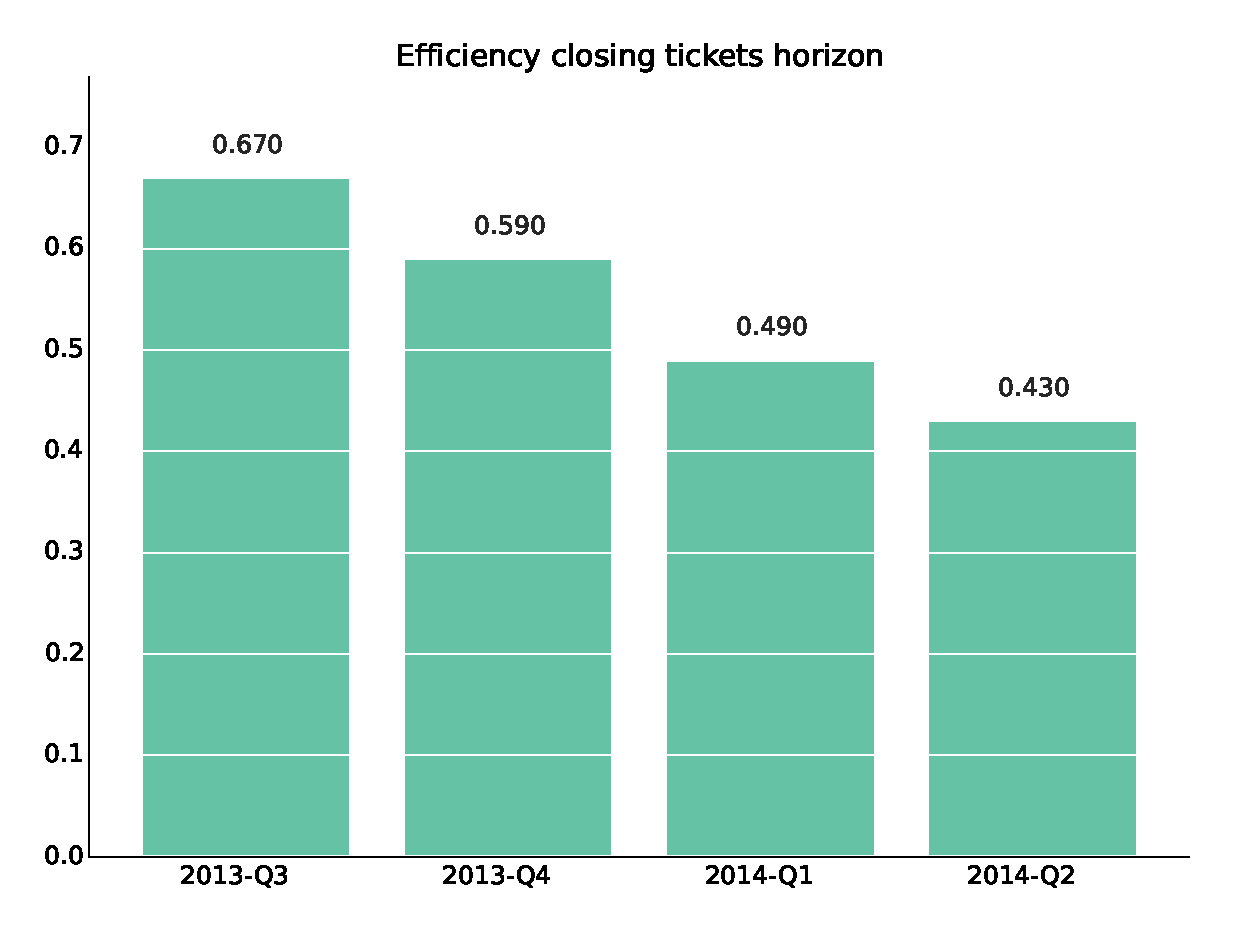
\includegraphics[scale=.35]{figs/bmihorizon.eps}
    & 
    \vspace{0pt}
    \begin{tabular}{l|l}%
    \bfseries Period & \bfseries Closed/Opened % specify table head
    \csvreader[head to column names]{data/bmihorizon.csv}{}% use head of csv as column names
    {\\\labels & \bmi}
    \end{tabular}
\end{tabular}

\begin{tabular}{p{7cm} p{5cm}}
    \vspace{0pt} 
    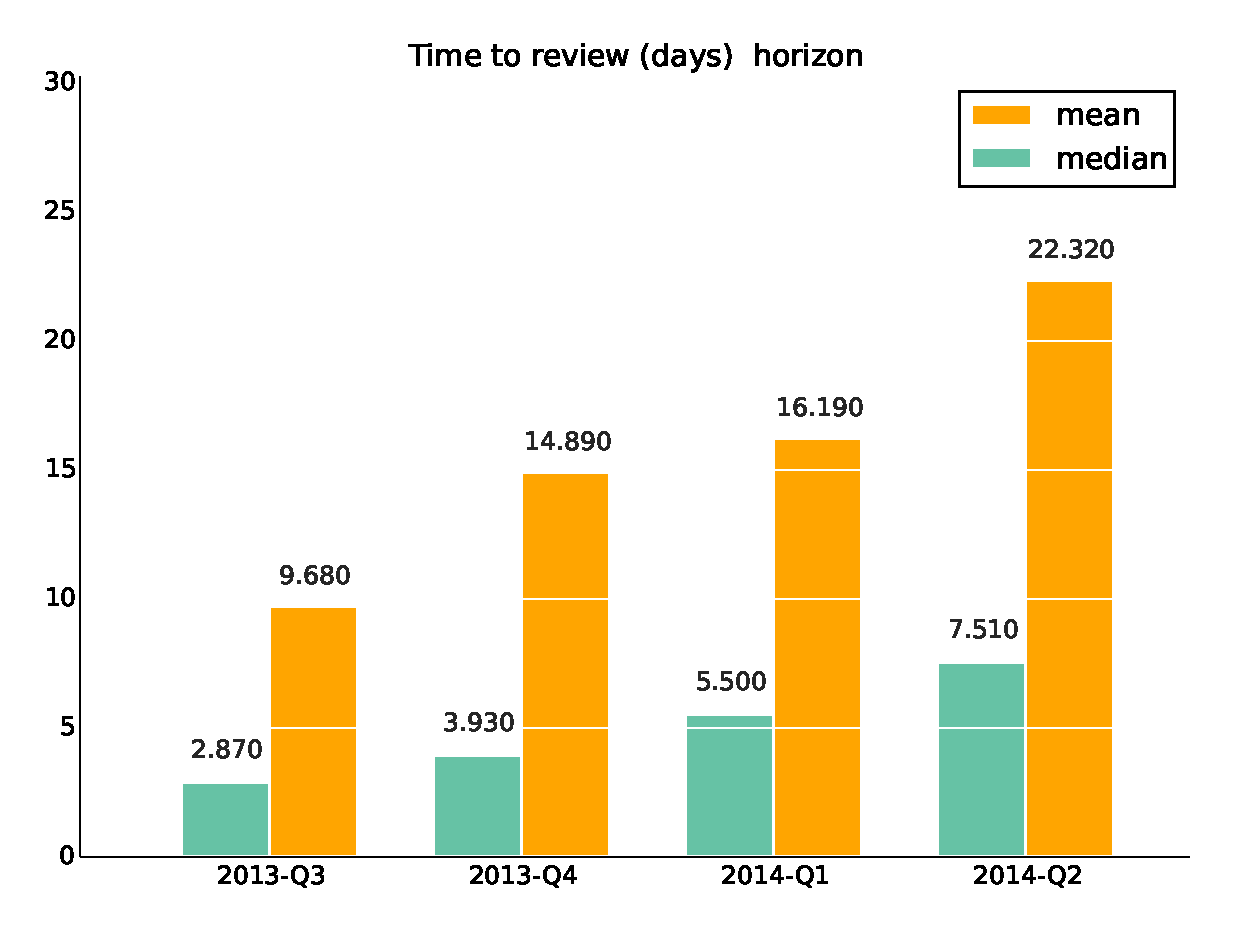
\includegraphics[scale=.35]{figs/timetoreview_medianhorizon.eps}
    & 
    \vspace{0pt}
    \begin{tabular}{l|r|r|}%
    \bfseries Period & \bfseries Median & \bfseries Mean % specify table head
    \csvreader[head to column names]{data/timetoreview_medianhorizon.csv}{}% use head of csv as column names
    {\\\labels & \mediantime & \meantime}
    \end{tabular}
\end{tabular}


 \newpage 
 \subsubsection{Keystone}

\begin{tabular}{p{7cm} p{5cm}}
    \vspace{0pt} 
    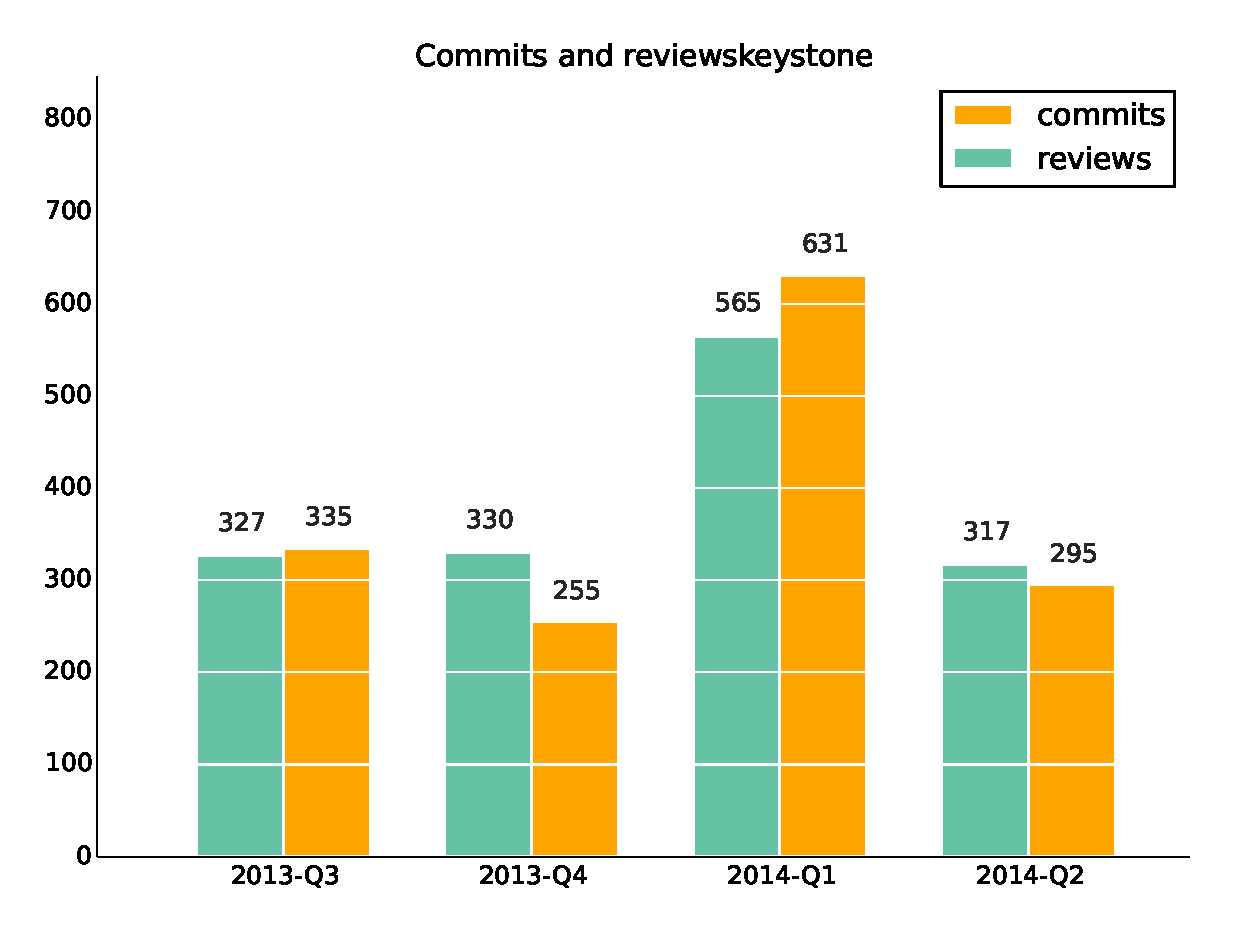
\includegraphics[scale=.35]{figs/commitskeystone.eps}
    & 
    \vspace{0pt}
    \begin{tabular}{l|r|r|}%
    \bfseries Period & \bfseries Commits & \bfseries Reviews % specify table head
    \csvreader[head to column names]{data/commitskeystone.csv}{}% use head of csv as column names
    {\\\labels & \commits & \submitted}
    \end{tabular}
\end{tabular}

\begin{tabular}{p{7cm} p{5cm}}
    \vspace{0pt} 
    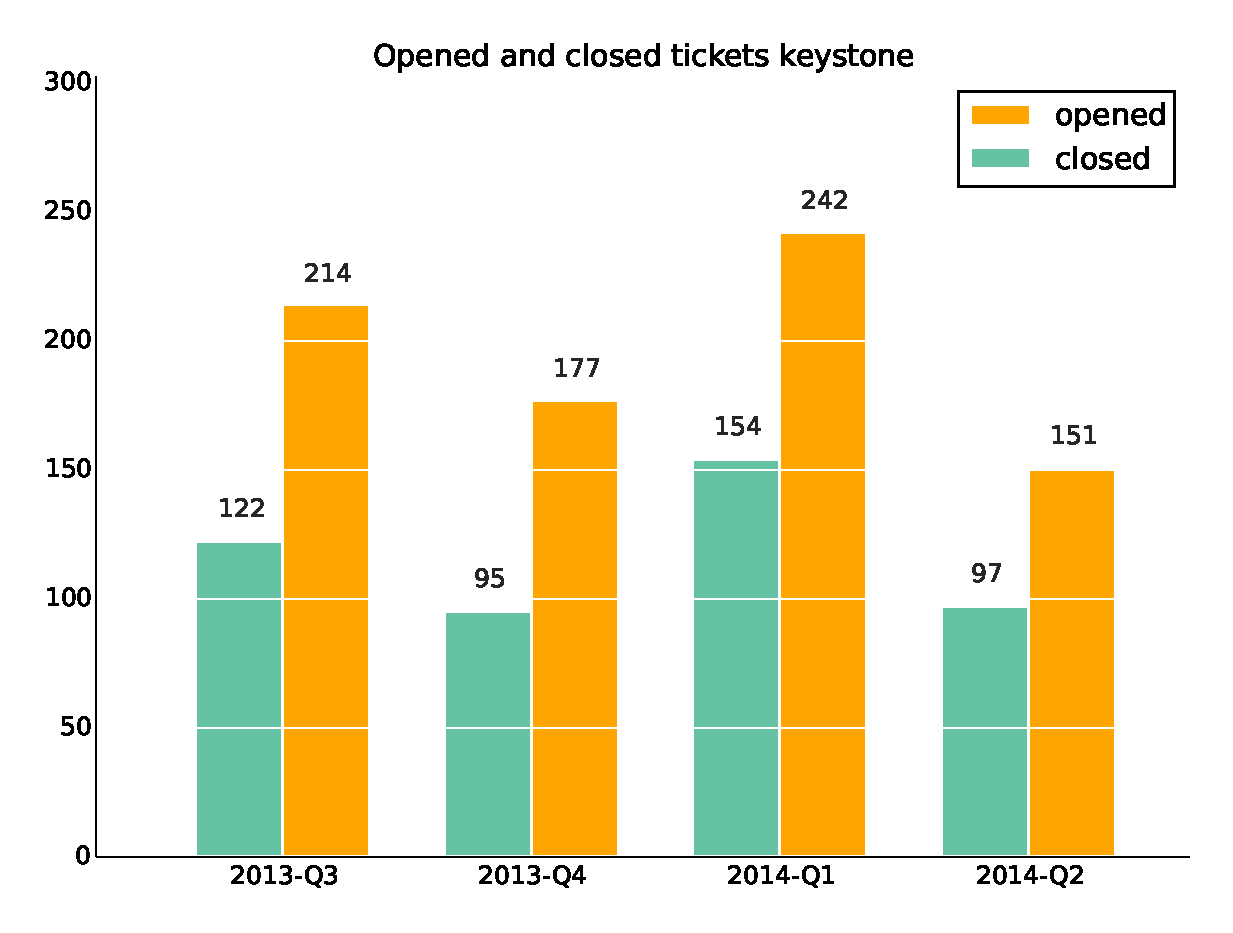
\includegraphics[scale=.35]{figs/closedkeystone.eps}
    & 
    \vspace{0pt}
    \begin{tabular}{l|r|r|}%
\bfseries Period & \bfseries Closed & \bfseries Opened
    \csvreader[head to column names]{data/closedkeystone.csv}{}% use head of csv as column names
    {\\\labels & \closed & \opened}
    \end{tabular}
\end{tabular}

\begin{tabular}{p{7cm} p{5cm}}
    \vspace{0pt} 
    \includegraphics[scale=.35]{figs/submitted_reviewskeystone.eps}
    & 
    \vspace{0pt}
    \begin{tabular}{l|r|r|}%
    \bfseries Period & \bfseries Merged & \bfseries Abandoned % specify table head
    \csvreader[head to column names]{data/submitted_reviewskeystone.csv}{}% use head of csv as column names
    {\\\labels & \merged & \abandoned}
    \end{tabular}
\end{tabular}


\textbf{Community}: Authors per quarter and top authors and organizations in the last quarter

\begin{tabular}{p{7cm} p{5cm}}
    \vspace{0pt} 
    \includegraphics[scale=.35]{figs/authorskeystone.eps}
    & 
    \vspace{0pt}
    \begin{tabular}{l|l}%
    \bfseries Period & \bfseries Authors % specify table head
    \csvreader[head to column names]{data/authorskeystone.csv}{}% use head of csv as column names
    {\\\labels & \authors}
    \end{tabular}
\end{tabular}

\begin{tabular}{p{7cm} p{5cm}}
    \vspace{0pt}
\begin{tabular}{l|l}%
    \bfseries Commit (s) & \bfseries Author % specify table head
    \csvreader[head to column names]{data/scm_top_authors_project_keystone.csv}{}% use head of csv as column names
    {\\\hline\csvcoli&\csvcolii}% specify your coloumns here
\end{tabular}
&
\vspace{0pt}
\begin{tabular}{l|l}%
    \bfseries Commit (s) & \bfseries Organizations % specify table head
    \csvreader[head to column names]{data/scm_top_companies_project_keystone.csv}{}% use head of csv as column names
    {\\\hline\csvcoli&\csvcolii}% specify your coloumns here
\end{tabular}
\end {tabular}

\textbf{Process}: Efficiency closing issues and time to review: mean and median

\begin{tabular}{p{7cm} p{5cm}}
    \vspace{0pt} 
    \includegraphics[scale=.35]{figs/bmikeystone.eps}
    & 
    \vspace{0pt}
    \begin{tabular}{l|l}%
    \bfseries Period & \bfseries Closed/Opened % specify table head
    \csvreader[head to column names]{data/bmikeystone.csv}{}% use head of csv as column names
    {\\\labels & \bmi}
    \end{tabular}
\end{tabular}

\begin{tabular}{p{7cm} p{5cm}}
    \vspace{0pt} 
    \includegraphics[scale=.35]{figs/timetoreview_mediankeystone.eps}
    & 
    \vspace{0pt}
    \begin{tabular}{l|r|r|}%
    \bfseries Period & \bfseries Median & \bfseries Mean % specify table head
    \csvreader[head to column names]{data/timetoreview_mediankeystone.csv}{}% use head of csv as column names
    {\\\labels & \mediantime & \meantime}
    \end{tabular}
\end{tabular}

\newpage 
 \subsubsection{Neutron}

\textbf{Activity}: Commits in Git, submitted, merged and abandoned reviews in Gerrit and opened and closed issues in Launchpad.

\begin{tabular}{p{7cm} p{5cm}}
    \vspace{0pt} 
    \includegraphics[scale=.35]{figs/commitsneutron.eps}
    & 
    \vspace{0pt}
    \begin{tabular}{l|r|r|}%
    \bfseries Period & \bfseries Commits & \bfseries Reviews % specify table head
    \csvreader[head to column names]{data/commitsneutron.csv}{}% use head of csv as column names
    {\\\labels & \commits & \submitted}
    \end{tabular}
\end{tabular}

\begin{tabular}{p{7cm} p{5cm}}
    \vspace{0pt} 
    \includegraphics[scale=.35]{figs/closedneutron.eps}
    & 
    \vspace{0pt}
    \begin{tabular}{l|r|r|}%
    \bfseries Period & \bfseries Closed & \bfseries Opened
    \csvreader[head to column names]{data/closedneutron.csv}{}% use head of csv as column names
    {\\\labels & \closed & \opened}
    \end{tabular}
\end{tabular}

\begin{tabular}{p{7cm} p{5cm}}
    \vspace{0pt} 
    \includegraphics[scale=.35]{figs/submitted_reviewsneutron.eps}
    & 
    \vspace{0pt}
    \begin{tabular}{l|r|r|}%
    \bfseries Period & \bfseries Merged & \bfseries Abandoned % specify table head
    \csvreader[head to column names]{data/submitted_reviewsneutron.csv}{}% use head of csv as column names
    {\\\labels & \merged & \abandoned}
    \end{tabular}
\end{tabular}


\textbf{Community}: Authors per quarter and top authors and organizations in the last quarter

\begin{tabular}{p{7cm} p{5cm}}
    \vspace{0pt} 
    \includegraphics[scale=.35]{figs/authorsneutron.eps}
    & 
    \vspace{0pt}
    \begin{tabular}{l|l}%
    \bfseries Period & \bfseries Authors % specify table head
    \csvreader[head to column names]{data/authorsneutron.csv}{}% use head of csv as column names
    {\\\labels & \authors}
    \end{tabular}
\end{tabular}

\begin{tabular}{p{7cm} p{5cm}}
    \vspace{0pt}
\begin{tabular}{l|l}%
    \bfseries Commit (s) & \bfseries Author % specify table head
    \csvreader[head to column names]{data/scm_top_authors_project_neutron.csv}{}% use head of csv as column names
    {\\\hline\csvcoli&\csvcolii}% specify your coloumns here
\end{tabular}
&
\vspace{0pt}
\begin{tabular}{l|l}%
    \bfseries Commit (s) & \bfseries Organizations % specify table head
    \csvreader[head to column names]{data/scm_top_companies_project_neutron.csv}{}% use head of csv as column names
    {\\\hline\csvcoli&\csvcolii}% specify your coloumns here
\end{tabular}
\end {tabular}

\textbf{Process}: Efficiency closing issues and time to review: mean and median

\begin{tabular}{p{7cm} p{5cm}}
    \vspace{0pt} 
    \includegraphics[scale=.35]{figs/bmineutron.eps}
    & 
    \vspace{0pt}
    \begin{tabular}{l|l}%
    \bfseries Period & \bfseries Closed/Opened % specify table head
    \csvreader[head to column names]{data/bmineutron.csv}{}% use head of csv as column names
    {\\\labels & \bmi}
    \end{tabular}
\end{tabular}

\begin{tabular}{p{7cm} p{5cm}}
    \vspace{0pt} 
    \includegraphics[scale=.35]{figs/timetoreview_medianneutron.eps}
    & 
    \vspace{0pt}
    \begin{tabular}{l|r|r|}%
    \bfseries Period & \bfseries Median & \bfseries Mean % specify table head
    \csvreader[head to column names]{data/timetoreview_medianneutron.csv}{}% use head of csv as column names
    {\\\labels & \mediantime & \meantime}
    \end{tabular}
\end{tabular}

\newpage 
 \subsubsection{Nova}

\textbf{Activity}: Commits in Git, submitted, merged and abandoned reviews in Gerrit and opened and closed issues in Launchpad.

\begin{tabular}{p{7cm} p{5cm}}
    \vspace{0pt} 
    \includegraphics[scale=.35]{figs/commitsnova.eps}
    & 
    \vspace{0pt}
    \begin{tabular}{l|r|r|}%
    \bfseries Period & \bfseries Commits & \bfseries Reviews % specify table head
    \csvreader[head to column names]{data/commitsnova.csv}{}% use head of csv as column names
    {\\\labels & \commits & \submitted}
    \end{tabular}
\end{tabular}

\begin{tabular}{p{7cm} p{5cm}}
    \vspace{0pt} 
    \includegraphics[scale=.35]{figs/closednova.eps}
    & 
    \vspace{0pt}
    \begin{tabular}{l|r|r|}%
\bfseries Period & \bfseries Closed & \bfseries Opened
    \csvreader[head to column names]{data/closednova.csv}{}% use head of csv as column names
    {\\\labels & \closed & \opened}
    \end{tabular}
\end{tabular}

\begin{tabular}{p{7cm} p{5cm}}
    \vspace{0pt} 
    \includegraphics[scale=.35]{figs/submitted_reviewsnova.eps}
    & 
    \vspace{0pt}
    \begin{tabular}{l|r|r|}%
    \bfseries Period & \bfseries Merged & \bfseries Abandoned % specify table head
    \csvreader[head to column names]{data/submitted_reviewsnova.csv}{}% use head of csv as column names
    {\\\labels & \merged & \abandoned}
    \end{tabular}
\end{tabular}


\textbf{Community}: Authors per quarter and top authors and organizations in the last quarter

\begin{tabular}{p{7cm} p{5cm}}
    \vspace{0pt} 
    \includegraphics[scale=.35]{figs/authorsnova.eps}
    & 
    \vspace{0pt}
    \begin{tabular}{l|l}%
    \bfseries Period & \bfseries Authors % specify table head
    \csvreader[head to column names]{data/authorsnova.csv}{}% use head of csv as column names
    {\\\labels & \authors}
    \end{tabular}
\end{tabular}

\begin{tabular}{p{7cm} p{5cm}}
    \vspace{0pt}
\begin{tabular}{l|l}%
    \bfseries Commit (s) & \bfseries Author % specify table head
    \csvreader[head to column names]{data/scm_top_authors_project_nova.csv}{}% use head of csv as column names
    {\\\hline\csvcoli&\csvcolii}% specify your coloumns here
\end{tabular}
&
\vspace{0pt}
\begin{tabular}{l|l}%
    \bfseries Commit (s) & \bfseries Organizations % specify table head
    \csvreader[head to column names]{data/scm_top_companies_project_nova.csv}{}% use head of csv as column names
    {\\\hline\csvcoli&\csvcolii}% specify your coloumns here
\end{tabular}
\end {tabular}

\textbf{Process}: Efficiency closing issues and time to review: mean and median

\begin{tabular}{p{7cm} p{5cm}}
    \vspace{0pt} 
    \includegraphics[scale=.35]{figs/bminova.eps}
    & 
    \vspace{0pt}
    \begin{tabular}{l|l}%
    \bfseries Period & \bfseries Closed/Opened % specify table head
    \csvreader[head to column names]{data/bminova.csv}{}% use head of csv as column names
    {\\\labels & \bmi}
    \end{tabular}
\end{tabular}

\begin{tabular}{p{7cm} p{5cm}}
    \vspace{0pt} 
    \includegraphics[scale=.35]{figs/timetoreview_mediannova.eps}
    & 
    \vspace{0pt}
    \begin{tabular}{l|r|r|}%
    \bfseries Period & \bfseries Median & \bfseries Mean % specify table head
    \csvreader[head to column names]{data/timetoreview_mediannova.csv}{}% use head of csv as column names
    {\\\labels & \mediantime & \meantime}
    \end{tabular}
\end{tabular}

\newpage 
 \subsubsection{Sahara}

\textbf{Activity}: Commits in Git, submitted, merged and abandoned reviews in Gerrit and opened and closed issues in Launchpad.

\begin{tabular}{p{7cm} p{5cm}}
    \vspace{0pt} 
    \includegraphics[scale=.35]{figs/commitssahara.eps}
    & 
    \vspace{0pt}
    \begin{tabular}{l|r|r|}%
    \bfseries Period & \bfseries Commits & \bfseries Reviews % specify table head
    \csvreader[head to column names]{data/commitssahara.csv}{}% use head of csv as column names
    {\\\labels & \commits & \submitted}
    \end{tabular}
\end{tabular}

\begin{tabular}{p{7cm} p{5cm}}
    \vspace{0pt} 
    \includegraphics[scale=.35]{figs/closedsahara.eps}
    & 
    \vspace{0pt}
    \begin{tabular}{l|r|r|}%
\bfseries Period & \bfseries Closed & \bfseries Opened
    \csvreader[head to column names]{data/closedsahara.csv}{}% use head of csv as column names
    {\\\labels & \closed & \opened}
    \end{tabular}
\end{tabular}

\begin{tabular}{p{7cm} p{5cm}}
    \vspace{0pt} 
    \includegraphics[scale=.35]{figs/submitted_reviewssahara.eps}
    & 
    \vspace{0pt}
    \begin{tabular}{l|r|r|}%
    \bfseries Period & \bfseries Merged & \bfseries Abandoned % specify table head
    \csvreader[head to column names]{data/submitted_reviewssahara.csv}{}% use head of csv as column names
    {\\\labels & \merged & \abandoned}
    \end{tabular}
\end{tabular}


\textbf{Community}: Authors per quarter and top authors and organizations in the last quarter

\begin{tabular}{p{7cm} p{5cm}}
    \vspace{0pt} 
    \includegraphics[scale=.35]{figs/authorssahara.eps}
    & 
    \vspace{0pt}
    \begin{tabular}{l|l}%
    \bfseries Period & \bfseries Authors % specify table head
    \csvreader[head to column names]{data/authorssahara.csv}{}% use head of csv as column names
    {\\\labels & \authors}
    \end{tabular}
\end{tabular}

\begin{tabular}{p{7cm} p{5cm}}
    \vspace{0pt}
\begin{tabular}{l|l}%
    \bfseries Commit (s) & \bfseries Author % specify table head
    \csvreader[head to column names]{data/scm_top_authors_project_sahara.csv}{}% use head of csv as column names
    {\\\hline\csvcoli&\csvcolii}% specify your coloumns here
\end{tabular}
&
\vspace{0pt}
\begin{tabular}{l|l}%
    \bfseries Commit (s) & \bfseries Organizations % specify table head
    \csvreader[head to column names]{data/scm_top_companies_project_sahara.csv}{}% use head of csv as column names
    {\\\hline\csvcoli&\csvcolii}% specify your coloumns here
\end{tabular}
\end {tabular}

\textbf{Process}: Efficiency closing issues and time to review: mean and median

\begin{tabular}{p{7cm} p{5cm}}
    \vspace{0pt} 
    \includegraphics[scale=.35]{figs/bmisahara.eps}
    & 
    \vspace{0pt}
    \begin{tabular}{l|l}%
    \bfseries Period & \bfseries Closed/Opened % specify table head
    \csvreader[head to column names]{data/bmisahara.csv}{}% use head of csv as column names
    {\\\labels & \bmi}
    \end{tabular}
\end{tabular}

\begin{tabular}{p{7cm} p{5cm}}
    \vspace{0pt} 
    \includegraphics[scale=.35]{figs/timetoreview_mediansahara.eps}
    & 
    \vspace{0pt}
    \begin{tabular}{l|r|r|}%
    \bfseries Period & \bfseries Median & \bfseries Mean % specify table head
    \csvreader[head to column names]{data/timetoreview_mediansahara.csv}{}% use head of csv as column names
    {\\\labels & \mediantime & \meantime}
    \end{tabular}
\end{tabular}

\newpage 
 \subsubsection{Swift}

\textbf{Activity}: Commits in Git, submitted, merged and abandoned reviews in Gerrit and opened and closed issues in Launchpad.

\begin{tabular}{p{7cm} p{5cm}}
    \vspace{0pt} 
    \includegraphics[scale=.35]{figs/commitsswift.eps}
    & 
    \vspace{0pt}
    \begin{tabular}{l|r|r|}%
    \bfseries Period & \bfseries Commits & \bfseries Reviews % specify table head
    \csvreader[head to column names]{data/commitsswift.csv}{}% use head of csv as column names
    {\\\labels & \commits & \submitted}
    \end{tabular}
\end{tabular}

\begin{tabular}{p{7cm} p{5cm}}
    \vspace{0pt} 
    \includegraphics[scale=.35]{figs/closedswift.eps}
    & 
    \vspace{0pt}
    \begin{tabular}{l|r|r|}%
\bfseries Period & \bfseries Closed & \bfseries Opened
    \csvreader[head to column names]{data/closedswift.csv}{}% use head of csv as column names
    {\\\labels & \closed & \opened}
    \end{tabular}
\end{tabular}

\begin{tabular}{p{7cm} p{5cm}}
    \vspace{0pt} 
    \includegraphics[scale=.35]{figs/submitted_reviewsswift.eps}
    & 
    \vspace{0pt}
    \begin{tabular}{l|r|r|}%
    \bfseries Period & \bfseries Merged & \bfseries Abandoned % specify table head
    \csvreader[head to column names]{data/submitted_reviewsswift.csv}{}% use head of csv as column names
    {\\\labels & \merged & \abandoned}
    \end{tabular}
\end{tabular}


\textbf{Community}: Authors per quarter and top authors and organizations in the last quarter

\begin{tabular}{p{7cm} p{5cm}}
    \vspace{0pt} 
    \includegraphics[scale=.35]{figs/authorsswift.eps}
    & 
    \vspace{0pt}
    \begin{tabular}{l|l}%
    \bfseries Period & \bfseries Authors % specify table head
    \csvreader[head to column names]{data/authorsswift.csv}{}% use head of csv as column names
    {\\\labels & \authors}
    \end{tabular}
\end{tabular}

\begin{tabular}{p{7cm} p{5cm}}
    \vspace{0pt}
\begin{tabular}{l|l}%
    \bfseries Commit (s) & \bfseries Author % specify table head
    \csvreader[head to column names]{data/scm_top_authors_project_swift.csv}{}% use head of csv as column names
    {\\\hline\csvcoli&\csvcolii}% specify your coloumns here
\end{tabular}
&
\vspace{0pt}
\begin{tabular}{l|l}%
    \bfseries Commit (s) & \bfseries Organizations % specify table head
    \csvreader[head to column names]{data/scm_top_companies_project_swift.csv}{}% use head of csv as column names
    {\\\hline\csvcoli&\csvcolii}% specify your coloumns here
\end{tabular}
\end {tabular}

\textbf{Process}: Efficiency closing issues and time to review: mean and median: Efficiency closing issues and time to review: mean and median

\begin{tabular}{p{7cm} p{5cm}}
    \vspace{0pt} 
    \includegraphics[scale=.35]{figs/bmiswift.eps}
    & 
    \vspace{0pt}
    \begin{tabular}{l|l}%
    \bfseries Period & \bfseries Closed/Opened % specify table head
    \csvreader[head to column names]{data/bmiswift.csv}{}% use head of csv as column names
    {\\\labels & \bmi}
    \end{tabular}
\end{tabular}

\begin{tabular}{p{7cm} p{5cm}}
    \vspace{0pt} 
    \includegraphics[scale=.35]{figs/timetoreview_medianswift.eps}
    & 
    \vspace{0pt}
    \begin{tabular}{l|r|r|}%
    \bfseries Period & \bfseries Median & \bfseries Mean % specify table head
    \csvreader[head to column names]{data/timetoreview_medianswift.csv}{}% use head of csv as column names
    {\\\labels & \mediantime & \meantime}
    \end{tabular}
\end{tabular}

\newpage 
 \subsubsection{Trove}

\textbf{Activity}: Commits in Git, submitted, merged and abandoned reviews in Gerrit and opened and closed issues in Launchpad.

\begin{tabular}{p{7cm} p{5cm}}
    \vspace{0pt} 
    \includegraphics[scale=.35]{figs/commitstrove.eps}
    & 
    \vspace{0pt}
    \begin{tabular}{l|r|r|}%
    \bfseries Period & \bfseries Commits & \bfseries Reviews % specify table head
    \csvreader[head to column names]{data/commitstrove.csv}{}% use head of csv as column names
    {\\\labels & \commits & \submitted}
    \end{tabular}
\end{tabular}

\begin{tabular}{p{7cm} p{5cm}}
    \vspace{0pt} 
    \includegraphics[scale=.35]{figs/closedtrove.eps}
    & 
    \vspace{0pt}
    \begin{tabular}{l|r|r|}%
\bfseries Period & \bfseries Closed & \bfseries Opened
    \csvreader[head to column names]{data/closedtrove.csv}{}% use head of csv as column names
    {\\\labels & \closed & \opened}
    \end{tabular}
\end{tabular}

\begin{tabular}{p{7cm} p{5cm}}
    \vspace{0pt} 
    \includegraphics[scale=.35]{figs/submitted_reviewstrove.eps}
    & 
    \vspace{0pt}
    \begin{tabular}{l|r|r|}%
    \bfseries Period & \bfseries Merged & \bfseries Abandoned % specify table head
    \csvreader[head to column names]{data/submitted_reviewstrove.csv}{}% use head of csv as column names
    {\\\labels & \merged & \abandoned}
    \end{tabular}
\end{tabular}

\textbf{Community}: Authors per quarter and top authors and organizations in the last quarter

\begin{tabular}{p{7cm} p{5cm}}
    \vspace{0pt} 
    \includegraphics[scale=.35]{figs/authorstrove.eps}
    & 
    \vspace{0pt}
    \begin{tabular}{l|l}%
    \bfseries Period & \bfseries Authors % specify table head
    \csvreader[head to column names]{data/authorstrove.csv}{}% use head of csv as column names
    {\\\labels & \authors}
    \end{tabular}
\end{tabular}

\begin{tabular}{p{7cm} p{5cm}}
    \vspace{0pt}
\begin{tabular}{l|l}%
    \bfseries Commit (s) & \bfseries Author % specify table head
    \csvreader[head to column names]{data/scm_top_authors_project_trove.csv}{}% use head of csv as column names
    {\\\hline\csvcoli&\csvcolii}% specify your coloumns here
\end{tabular}
&
\vspace{0pt}
\begin{tabular}{l|l}%
    \bfseries Commit (s) & \bfseries Organizations % specify table head
    \csvreader[head to column names]{data/scm_top_companies_project_trove.csv}{}% use head of csv as column names
    {\\\hline\csvcoli&\csvcolii}% specify your coloumns here
\end{tabular}
\end {tabular}

\textbf{Process}: Efficiency closing issues and time to review: mean and median

\begin{tabular}{p{7cm} p{5cm}}
    \vspace{0pt} 
    \includegraphics[scale=.35]{figs/bmitrove.eps}
    & 
    \vspace{0pt}
    \begin{tabular}{l|l}%
    \bfseries Period & \bfseries Closed/Opened % specify table head
    \csvreader[head to column names]{data/bmitrove.csv}{}% use head of csv as column names
    {\\\labels & \bmi}
    \end{tabular}
\end{tabular}

\begin{tabular}{p{7cm} p{5cm}}
    \vspace{0pt} 
    \includegraphics[scale=.35]{figs/timetoreview_mediantrove.eps}
    & 
    \vspace{0pt}
    \begin{tabular}{l|r|r|}%
    \bfseries Period & \bfseries Median & \bfseries Mean % specify table head
    \csvreader[head to column names]{data/timetoreview_mediantrove.csv}{}% use head of csv as column names
    {\\\labels & \mediantime & \meantime}
    \end{tabular}
\end{tabular}

\newpage
\subsection{Incubated}

\textbf{Activity}: Commits in Git, submitted, merged and abandoned reviews in Gerrit and opened and closed issues in Launchpad.

\begin{tabular}{p{7cm} p{5cm}}
    \vspace{0pt} 
    \includegraphics[scale=.35]{figs/commitsincubated.eps}
    & 
    \vspace{0pt}
    \begin{tabular}{l|r|r|}%
    \bfseries Period & \bfseries Commits & \bfseries Reviews % specify table head
    \csvreader[head to column names]{data/commitsincubated.csv}{}% use head of csv as column names
    {\\\labels & \commits & \submitted}
    \end{tabular}
\end{tabular}

\begin{tabular}{p{7cm} p{5cm}}
    \vspace{0pt} 
    \includegraphics[scale=.35]{figs/closedincubated.eps}
    & 
    \vspace{0pt}
    \begin{tabular}{l|r|r|}%
\bfseries Period & \bfseries Closed & \bfseries Opened
    \csvreader[head to column names]{data/closedincubated.csv}{}% use head of csv as column names
    {\\\labels & \closed & \opened}
    \end{tabular}
\end{tabular}

\begin{tabular}{p{7cm} p{5cm}}
    \vspace{0pt} 
    \includegraphics[scale=.35]{figs/submitted_reviewsincubated.eps}
    & 
    \vspace{0pt}
    \begin{tabular}{l|r|r|}%
    \bfseries Period & \bfseries Merged & \bfseries Abandoned % specify table head
    \csvreader[head to column names]{data/submitted_reviewsincubated.csv}{}% use head of csv as column names
    {\\\labels & \merged & \abandoned}
    \end{tabular}
\end{tabular}


\textbf{Community}: Authors per quarter and top authors and organizations in the last quarter

\begin{tabular}{p{7cm} p{5cm}}
    \vspace{0pt} 
    \includegraphics[scale=.35]{figs/authorsincubated.eps}
    & 
    \vspace{0pt}
    \begin{tabular}{l|l}%
    \bfseries Period & \bfseries Authors % specify table head
    \csvreader[head to column names]{data/authorsincubated.csv}{}% use head of csv as column names
    {\\\labels & \authors}
    \end{tabular}
\end{tabular}

\begin{tabular}{p{7cm} p{5cm}}
    \vspace{0pt}
\begin{tabular}{l|l}%
    \bfseries Commit (s) & \bfseries Author % specify table head
    \csvreader[head to column names]{data/scm_top_authors_project_incubated.csv}{}% use head of csv as column names
    {\\\hline\csvcoli&\csvcolii}% specify your coloumns here
\end{tabular}
&
\vspace{0pt}
\begin{tabular}{l|l}%
    \bfseries Commit (s) & \bfseries Organizations % specify table head
    \csvreader[head to column names]{data/scm_top_companies_project_incubated.csv}{}% use head of csv as column names
    {\\\hline\csvcoli&\csvcolii}% specify your coloumns here
\end{tabular}
\end {tabular}

\textbf{Process}: Efficiency closing issues and time to review: mean and median



\begin{tabular}{p{7cm} p{5cm}}
    \vspace{0pt} 
    \includegraphics[scale=.35]{figs/timetoreview_medianincubated.eps}
    & 
    \vspace{0pt}
    \begin{tabular}{l|r|r|}%
    \bfseries Period & \bfseries Median & \bfseries Mean % specify table head
    \csvreader[head to column names]{data/timetoreview_medianincubated.csv}{}% use head of csv as column names
    {\\\labels & \mediantime & \meantime}
    \end{tabular}
\end{tabular}

\newpage
\subsection{Clients}

\textbf{Activity}: Commits in Git, submitted, merged and abandoned reviews in Gerrit and opened and closed issues in Launchpad.

\begin{tabular}{p{7cm} p{5cm}}
    \vspace{0pt} 
    \includegraphics[scale=.35]{figs/commitsclients.eps}
    & 
    \vspace{0pt}
    \begin{tabular}{l|r|r|}%
    \bfseries Period & \bfseries Commits & \bfseries Reviews % specify table head
    \csvreader[head to column names]{data/commitsclients.csv}{}% use head of csv as column names
    {\\\labels & \commits & \submitted}
    \end{tabular}
\end{tabular}

\begin{tabular}{p{7cm} p{5cm}}
    \vspace{0pt} 
    \includegraphics[scale=.35]{figs/closedclients.eps}
    & 
    \vspace{0pt}
    \begin{tabular}{l|r|r|}%
\bfseries Period & \bfseries Closed & \bfseries Opened
    \csvreader[head to column names]{data/closedclients.csv}{}% use head of csv as column names
    {\\\labels & \closed & \opened}
    \end{tabular}
\end{tabular}

\begin{tabular}{p{7cm} p{5cm}}
    \vspace{0pt} 
    \includegraphics[scale=.35]{figs/submitted_reviewsclients.eps}
    & 
    \vspace{0pt}
    \begin{tabular}{l|r|r|}%
    \bfseries Period & \bfseries Merged & \bfseries Abandoned % specify table head
    \csvreader[head to column names]{data/submitted_reviewsclients.csv}{}% use head of csv as column names
    {\\\labels & \merged & \abandoned}
    \end{tabular}
\end{tabular}


\textbf{Community}: Authors per quarter and top authors and organizations in the last quarter

\begin{tabular}{p{7cm} p{5cm}}
    \vspace{0pt} 
    \includegraphics[scale=.35]{figs/authorsclients.eps}
    & 
    \vspace{0pt}
    \begin{tabular}{l|l}%
    \bfseries Period & \bfseries Authors % specify table head
    \csvreader[head to column names]{data/authorsclients.csv}{}% use head of csv as column names
    {\\\labels & \authors}
    \end{tabular}
\end{tabular}

\begin{tabular}{p{7cm} p{5cm}}
    \vspace{0pt}
\begin{tabular}{l|l}%
    \bfseries Commit (s) & \bfseries Author % specify table head
    \csvreader[head to column names]{data/scm_top_authors_project_clients.csv}{}% use head of csv as column names
    {\\\hline\csvcoli&\csvcolii}% specify your coloumns here
\end{tabular}
&
\vspace{0pt}
\begin{tabular}{l|l}%
    \bfseries Commit (s) & \bfseries Organizations % specify table head
    \csvreader[head to column names]{data/scm_top_companies_project_clients.csv}{}% use head of csv as column names
    {\\\hline\csvcoli&\csvcolii}% specify your coloumns here
\end{tabular}
\end {tabular}

\textbf{Process}: Efficiency closing issues and time to review: mean and median

\begin{tabular}{p{7cm} p{5cm}}
    \vspace{0pt} 
    \includegraphics[scale=.35]{figs/bmiclients.eps}
    & 
    \vspace{0pt}
    He was an Austrian physicist famous for his founding contributions in the fields of
    statistical mechanics and statistical thermodynamics. He was one of the most
    important advocates for atomic theory at a time when that scientific model was 
    still highly controversial.\\
\end{tabular}

\begin{tabular}{p{7cm} p{5cm}}
    \vspace{0pt} 
    \includegraphics[scale=.35]{figs/timetoreview_medianclients.eps}
    & 
    \vspace{0pt}
    \begin{tabular}{l|r|r|}%
    \bfseries Period & \bfseries Median & \bfseries Mean % specify table head
    \csvreader[head to column names]{data/timetoreview_medianclients.csv}{}% use head of csv as column names
    {\\\labels & \mediantime & \meantime}
    \end{tabular}
\end{tabular}

\newpage
\subsection{Others}

\textbf{Activity}: Commits in Git, submitted, merged and abandoned reviews in Gerrit and opened and closed issues in Launchpad.

\begin{tabular}{p{7cm} p{5cm}}
    \vspace{0pt} 
    \includegraphics[scale=.35]{figs/commitsothers.eps}
    & 
    \vspace{0pt}
    \begin{tabular}{l|r|r|}%
    \bfseries Period & \bfseries Commits & \bfseries Reviews % specify table head
    \csvreader[head to column names]{data/commitsothers.csv}{}% use head of csv as column names
    {\\\labels & \commits & \submitted}
    \end{tabular}
\end{tabular}

\begin{tabular}{p{7cm} p{5cm}}
    \vspace{0pt} 
    \includegraphics[scale=.35]{figs/closedothers.eps}
    & 
    \vspace{0pt}
    \begin{tabular}{l|r|r|}%
\bfseries Period & \bfseries Closed & \bfseries Opened
    \csvreader[head to column names]{data/closedothers.csv}{}% use head of csv as column names
    {\\\labels & \closed & \opened}
    \end{tabular}
\end{tabular}

\begin{tabular}{p{7cm} p{5cm}}
    \vspace{0pt} 
    \includegraphics[scale=.35]{figs/submitted_reviewsothers.eps}
    & 
    \vspace{0pt}
    \begin{tabular}{l|r|r|}%
    \bfseries Period & \bfseries Merged & \bfseries Abandoned % specify table head
    \csvreader[head to column names]{data/submitted_reviewsothers.csv}{}% use head of csv as column names
    {\\\labels & \merged & \abandoned}
    \end{tabular}
\end{tabular}


\textbf{Community}: Authors per quarter and top authors and organizations in the last quarter

\begin{tabular}{p{7cm} p{5cm}}
    \vspace{0pt} 
    \includegraphics[scale=.35]{figs/authorsothers.eps}
    & 
    \vspace{0pt}
    \begin{tabular}{l|l}%
    \bfseries Period & \bfseries Authors % specify table head
    \csvreader[head to column names]{data/authorsothers.csv}{}% use head of csv as column names
    {\\\labels & \authors}
    \end{tabular}
\end{tabular}

\begin{tabular}{p{7cm} p{5cm}}
    \vspace{0pt}
\begin{tabular}{l|l}%
    \bfseries Commit (s) & \bfseries Author % specify table head
    \csvreader[head to column names]{data/scm_top_authors_project_others.csv}{}% use head of csv as column names
    {\\\hline\csvcoli&\csvcolii}% specify your coloumns here
\end{tabular}
&
\vspace{0pt}
\begin{tabular}{l|l}%
    \bfseries Commit (s) & \bfseries Organizations % specify table head
    \csvreader[head to column names]{data/scm_top_companies_project_others.csv}{}% use head of csv as column names
    {\\\hline\csvcoli&\csvcolii}% specify your coloumns here
\end{tabular}
\end {tabular}

\textbf{Process}: Efficiency closing issues and time to review: mean and median

\begin{tabular}{p{7cm} p{5cm}}
    \vspace{0pt} 
    \includegraphics[scale=.35]{figs/bmiothers.eps}
    & 
    \vspace{0pt}
    \begin{tabular}{l|l}%
    \bfseries Period & \bfseries Closed/Opened % specify table head
    \csvreader[head to column names]{data/bmiothers.csv}{}% use head of csv as column names
    {\\\labels & \bmi}
    \end{tabular}
\end{tabular}

\begin{tabular}{p{7cm} p{5cm}}
    \vspace{0pt} 
    \includegraphics[scale=.35]{figs/timetoreview_medianothers.eps}
    & 
    \vspace{0pt}
    \begin{tabular}{l|r|r|}%
    \bfseries Period & \bfseries Median & \bfseries Mean % specify table head
    \csvreader[head to column names]{data/timetoreview_medianothers.csv}{}% use head of csv as column names
    {\\\labels & \mediantime & \meantime}
    \end{tabular}
\end{tabular}

\newpage
\section{Common Libraries}

\textbf{Activity}: Commits in Git, submitted, merged and abandoned reviews in Gerrit and opened and closed issues in Launchpad.

\begin{tabular}{p{7cm} p{5cm}}
    \vspace{0pt} 
    \includegraphics[scale=.35]{figs/commitsCommonLibraries.eps}
    & 
    \vspace{0pt}
    \begin{tabular}{l|r|r|}%
    \bfseries Period & \bfseries Commits & \bfseries Reviews % specify table head
    \csvreader[head to column names]{data/commitsCommonLibraries.csv}{}% use head of csv as column names
    {\\\labels & \commits & \submitted}
    \end{tabular}
\end{tabular}

\begin{tabular}{p{7cm} p{5cm}}
    \vspace{0pt} 
    \includegraphics[scale=.35]{figs/closedCommonLibraries.eps}
    & 
    \vspace{0pt}
    \begin{tabular}{l|r|r|}%
\bfseries Period & \bfseries Closed & \bfseries Opened
    \csvreader[head to column names]{data/closedCommonLibraries.csv}{}% use head of csv as column names
    {\\\labels & \closed & \opened}
    \end{tabular}
\end{tabular}

\begin{tabular}{p{7cm} p{5cm}}
    \vspace{0pt} 
    \includegraphics[scale=.35]{figs/submitted_reviewsCommonLibraries.eps}
    & 
    \vspace{0pt}
    \begin{tabular}{l|r|r|}%
    \bfseries Period & \bfseries Merged & \bfseries Abandoned % specify table head
    \csvreader[head to column names]{data/submitted_reviewsCommonLibraries.csv}{}% use head of csv as column names
    {\\\labels & \merged & \abandoned}
    \end{tabular}
\end{tabular}


\textbf{Community}: Authors per quarter and top authors and organizations in the last quarter

\begin{tabular}{p{7cm} p{5cm}}
    \vspace{0pt} 
    \includegraphics[scale=.35]{figs/authorsCommonLibraries.eps}
    & 
    \vspace{0pt}
    \begin{tabular}{l|l}%
    \bfseries Period & \bfseries Authors % specify table head
    \csvreader[head to column names]{data/authorsCommonLibraries.csv}{}% use head of csv as column names
    {\\\labels & \authors}
    \end{tabular}
\end{tabular}

\begin{tabular}{p{7cm} p{5cm}}
    \vspace{0pt}
\begin{tabular}{l|l}%
    \bfseries Commit (s) & \bfseries Author % specify table head
    \csvreader[head to column names]{data/scm_top_authors_project_CommonLibraries.csv}{}% use head of csv as column names
    {\\\hline\csvcoli&\csvcolii}% specify your coloumns here
\end{tabular}
&
\vspace{0pt}
\begin{tabular}{l|l}%
    \bfseries Commit (s) & \bfseries Organizations % specify table head
    \csvreader[head to column names]{data/scm_top_companies_project_CommonLibraries.csv}{}% use head of csv as column names
    {\\\hline\csvcoli&\csvcolii}% specify your coloumns here
\end{tabular}
\end {tabular}

\textbf{Process}: Efficiency closing issues and time to review: mean and median

\begin{tabular}{p{7cm} p{5cm}}
    \vspace{0pt} 
    \includegraphics[scale=.35]{figs/bmiCommonLibraries.eps}
    & 
    \vspace{0pt}
    \begin{tabular}{l|l}%
    \bfseries Period & \bfseries Closed/Opened % specify table head
    \csvreader[head to column names]{data/bmiCommonLibraries.csv}{}% use head of csv as column names
    {\\\labels & \bmi}
    \end{tabular}
\end{tabular}

\begin{tabular}{p{7cm} p{5cm}}
    \vspace{0pt} 
    \includegraphics[scale=.35]{figs/timetoreview_medianCommonLibraries.eps}
    & 
    \vspace{0pt}
    \begin{tabular}{l|r|r|}%
    \bfseries Period & \bfseries Median & \bfseries Mean % specify table head
    \csvreader[head to column names]{data/timetoreview_medianCommonLibraries.csv}{}% use head of csv as column names
    {\\\labels & \mediantime & \meantime}
    \end{tabular}
\end{tabular}

\newpage
\section{Deployment}

\textbf{Activity}: Commits in Git, submitted, merged and abandoned reviews in Gerrit and opened and closed issues in Launchpad.

\begin{tabular}{p{7cm} p{5cm}}
    \vspace{0pt} 
    \includegraphics[scale=.35]{figs/commitsDeployment.eps}
    & 
    \vspace{0pt}
    \begin{tabular}{l|r|r|}%
    \bfseries Period & \bfseries Commits & \bfseries Reviews % specify table head
    \csvreader[head to column names]{data/commitsDeployment.csv}{}% use head of csv as column names
    {\\\labels & \commits & \submitted}
    \end{tabular}
\end{tabular}

\begin{tabular}{p{7cm} p{5cm}}
    \vspace{0pt} 
    \includegraphics[scale=.35]{figs/closedDeployment.eps}
    & 
    \vspace{0pt}
    \begin{tabular}{l|r|r|}%
\bfseries Period & \bfseries Closed & \bfseries Opened
    \csvreader[head to column names]{data/closedDeployment.csv}{}% use head of csv as column names
    {\\\labels & \closed & \opened}
    \end{tabular}
\end{tabular}

\begin{tabular}{p{7cm} p{5cm}}
    \vspace{0pt} 
    \includegraphics[scale=.35]{figs/submitted_reviewsDeployment.eps}
    & 
    \vspace{0pt}
    \begin{tabular}{l|r|r|}%
    \bfseries Period & \bfseries Merged & \bfseries Abandoned % specify table head
    \csvreader[head to column names]{data/submitted_reviewsDeployment.csv}{}% use head of csv as column names
    {\\\labels & \merged & \abandoned}
    \end{tabular}
\end{tabular}


\textbf{Community}: Authors per quarter and top authors and organizations in the last quarter

\begin{tabular}{p{7cm} p{5cm}}
    \vspace{0pt} 
    \includegraphics[scale=.35]{figs/authorsDeployment.eps}
    & 
    \vspace{0pt}
    \begin{tabular}{l|l}%
    \bfseries Period & \bfseries Authors % specify table head
    \csvreader[head to column names]{data/authorsDeployment.csv}{}% use head of csv as column names
    {\\\labels & \authors}
    \end{tabular}
\end{tabular}

\begin{tabular}{p{7cm} p{5cm}}
    \vspace{0pt}
\begin{tabular}{l|l}%
    \bfseries Commit (s) & \bfseries Author % specify table head
    \csvreader[head to column names]{data/scm_top_authors_project_Deployment.csv}{}% use head of csv as column names
    {\\\hline\csvcoli&\csvcolii}% specify your coloumns here
\end{tabular}
&
\vspace{0pt}
\begin{tabular}{l|l}%
    \bfseries Commit (s) & \bfseries Organizations % specify table head
    \csvreader[head to column names]{data/scm_top_companies_project_Deployment.csv}{}% use head of csv as column names
    {\\\hline\csvcoli&\csvcolii}% specify your coloumns here
\end{tabular}
\end {tabular}

\textbf{Process}: Efficiency closing issues and time to review: mean and median

\begin{tabular}{p{7cm} p{5cm}}
    \vspace{0pt} 
    \includegraphics[scale=.35]{figs/bmiDeployment.eps}
    & 
    \vspace{0pt}
    \begin{tabular}{l|l}%
    \bfseries Period & \bfseries Closed/Opened % specify table head
    \csvreader[head to column names]{data/bmiDeployment.csv}{}% use head of csv as column names
    {\\\labels & \bmi}
    \end{tabular}
\end{tabular}

\begin{tabular}{p{7cm} p{5cm}}
    \vspace{0pt} 
    \includegraphics[scale=.35]{figs/timetoreview_medianDeployment.eps}
    & 
    \vspace{0pt}
    \begin{tabular}{l|r|r|}%
    \bfseries Period & \bfseries Median & \bfseries Mean % specify table head
    \csvreader[head to column names]{data/timetoreview_medianDeployment.csv}{}% use head of csv as column names
    {\\\labels & \mediantime & \meantime}
    \end{tabular}
\end{tabular}

\newpage
\section{Devstack}

\textbf{Activity}: Commits in Git, submitted, merged and abandoned reviews in Gerrit and opened and closed issues in Launchpad.

\begin{tabular}{p{7cm} p{5cm}}
    \vspace{0pt} 
    \includegraphics[scale=.35]{figs/commitsDevstack.eps}
    & 
    \vspace{0pt}
    \begin{tabular}{l|r|r|}%
    \bfseries Period & \bfseries Commits & \bfseries Reviews % specify table head
    \csvreader[head to column names]{data/commitsDevstack.csv}{}% use head of csv as column names
    {\\\labels & \commits & \submitted}
    \end{tabular}
\end{tabular}

\begin{tabular}{p{7cm} p{5cm}}
    \vspace{0pt} 
    \includegraphics[scale=.35]{figs/closedDevstack.eps}
    & 
    \vspace{0pt}
    \begin{tabular}{l|r|r|}%
\bfseries Period & \bfseries Closed & \bfseries Opened
    \csvreader[head to column names]{data/closedDevstack.csv}{}% use head of csv as column names
    {\\\labels & \closed & \opened}
    \end{tabular}
\end{tabular}

\begin{tabular}{p{7cm} p{5cm}}
    \vspace{0pt} 
    \includegraphics[scale=.35]{figs/submitted_reviewsDevstack.eps}
    & 
    \vspace{0pt}
    \begin{tabular}{l|r|r|}%
    \bfseries Period & \bfseries Merged & \bfseries Abandoned % specify table head
    \csvreader[head to column names]{data/submitted_reviewsDevstack.csv}{}% use head of csv as column names
    {\\\labels & \merged & \abandoned}
    \end{tabular}
\end{tabular}


\textbf{Community}: Authors per quarter and top authors and organizations in the last quarter

\begin{tabular}{p{7cm} p{5cm}}
    \vspace{0pt} 
    \includegraphics[scale=.35]{figs/authorsDevstack.eps}
    & 
    \vspace{0pt}
    \begin{tabular}{l|l}%
    \bfseries Period & \bfseries Authors % specify table head
    \csvreader[head to column names]{data/authorsDevstack.csv}{}% use head of csv as column names
    {\\\labels & \authors}
    \end{tabular}
\end{tabular}

\begin{tabular}{p{7cm} p{5cm}}
    \vspace{0pt}
\begin{tabular}{l|l}%
    \bfseries Commit (s) & \bfseries Author % specify table head
    \csvreader[head to column names]{data/scm_top_authors_project_Devstack.csv}{}% use head of csv as column names
    {\\\hline\csvcoli&\csvcolii}% specify your coloumns here
\end{tabular}
&
\vspace{0pt}
\begin{tabular}{l|l}%
    \bfseries Commit (s) & \bfseries Organizations % specify table head
    \csvreader[head to column names]{data/scm_top_companies_project_Devstack.csv}{}% use head of csv as column names
    {\\\hline\csvcoli&\csvcolii}% specify your coloumns here
\end{tabular}
\end {tabular}

\textbf{Process}: Efficiency closing issues and time to review: mean and median

\begin{tabular}{p{7cm} p{5cm}}
    \vspace{0pt} 
    \includegraphics[scale=.35]{figs/bmiDevstack.eps}
    & 
    \vspace{0pt}
    \begin{tabular}{l|l}%
    \bfseries Period & \bfseries Closed/Opened % specify table head
    \csvreader[head to column names]{data/bmiDevstack.csv}{}% use head of csv as column names
    {\\\labels & \bmi}
    \end{tabular}
\end{tabular}

\begin{tabular}{p{7cm} p{5cm}}
    \vspace{0pt} 
    \includegraphics[scale=.35]{figs/timetoreview_medianDevstack.eps}
    & 
    \vspace{0pt}
    \begin{tabular}{l|r|r|}%
    \bfseries Period & \bfseries Median & \bfseries Mean % specify table head
    \csvreader[head to column names]{data/timetoreview_medianDevstack.csv}{}% use head of csv as column names
    {\\\labels & \mediantime & \meantime}
    \end{tabular}
\end{tabular}

\newpage
\section{Documentation}

\textbf{Activity}: Commits in Git, submitted, merged and abandoned reviews in Gerrit and opened and closed issues in Launchpad.

\begin{tabular}{p{7cm} p{5cm}}
    \vspace{0pt} 
    \includegraphics[scale=.35]{figs/commitsDocumentation.eps}
    & 
    \vspace{0pt}
    \begin{tabular}{l|r|r|}%
    \bfseries Period & \bfseries Commits & \bfseries Reviews % specify table head
    \csvreader[head to column names]{data/commitsDocumentation.csv}{}% use head of csv as column names
    {\\\labels & \commits & \submitted}
    \end{tabular}
\end{tabular}

\begin{tabular}{p{7cm} p{5cm}}
    \vspace{0pt} 
    \includegraphics[scale=.35]{figs/closedDocumentation.eps}
    & 
    \vspace{0pt}
    \begin{tabular}{l|r|r|}%
\bfseries Period & \bfseries Closed & \bfseries Opened
    \csvreader[head to column names]{data/closedDocumentation.csv}{}% use head of csv as column names
    {\\\labels & \closed & \opened}
    \end{tabular}
\end{tabular}

\begin{tabular}{p{7cm} p{5cm}}
    \vspace{0pt} 
    \includegraphics[scale=.35]{figs/submitted_reviewsDocumentation.eps}
    & 
    \vspace{0pt}
    \begin{tabular}{l|r|r|}%
    \bfseries Period & \bfseries Merged & \bfseries Abandoned % specify table head
    \csvreader[head to column names]{data/submitted_reviewsDocumentation.csv}{}% use head of csv as column names
    {\\\labels & \merged & \abandoned}
    \end{tabular}
\end{tabular}


\textbf{Community}: Authors per quarter and top authors and organizations in the last quarter

\begin{tabular}{p{7cm} p{5cm}}
    \vspace{0pt} 
    \includegraphics[scale=.35]{figs/authorsDocumentation.eps}
    & 
    \vspace{0pt}
    \begin{tabular}{l|l}%
    \bfseries Period & \bfseries Authors % specify table head
    \csvreader[head to column names]{data/authorsDocumentation.csv}{}% use head of csv as column names
    {\\\labels & \authors}
    \end{tabular}
\end{tabular}

\begin{tabular}{p{7cm} p{5cm}}
    \vspace{0pt}
\begin{tabular}{l|l}%
    \bfseries Commit (s) & \bfseries Author % specify table head
    \csvreader[head to column names]{data/scm_top_authors_project_Documentation.csv}{}% use head of csv as column names
    {\\\hline\csvcoli&\csvcolii}% specify your coloumns here
\end{tabular}
&
\vspace{0pt}
\begin{tabular}{l|l}%
    \bfseries Commit (s) & \bfseries Organizations % specify table head
    \csvreader[head to column names]{data/scm_top_companies_project_Documentation.csv}{}% use head of csv as column names
    {\\\hline\csvcoli&\csvcolii}% specify your coloumns here
\end{tabular}
\end {tabular}

\textbf{Process}: Efficiency closing issues and time to review: mean and median

\begin{tabular}{p{7cm} p{5cm}}
    \vspace{0pt} 
    \includegraphics[scale=.35]{figs/bmiDocumentation.eps}
    & 
    \vspace{0pt}
    \begin{tabular}{l|l}%
    \bfseries Period & \bfseries Closed/Opened % specify table head
    \csvreader[head to column names]{data/bmiDocumentation.csv}{}% use head of csv as column names
    {\\\labels & \bmi}
    \end{tabular}
\end{tabular}

\begin{tabular}{p{7cm} p{5cm}}
    \vspace{0pt} 
    \includegraphics[scale=.35]{figs/timetoreview_medianDocumentation.eps}
    & 
    \vspace{0pt}
    \begin{tabular}{l|r|r|}%
    \bfseries Period & \bfseries Median & \bfseries Mean % specify table head
    \csvreader[head to column names]{data/timetoreview_medianDocumentation.csv}{}% use head of csv as column names
    {\\\labels & \mediantime & \meantime}
    \end{tabular}
\end{tabular}

\newpage
\section{Infrastructure}

\textbf{Activity}: Commits in Git, submitted, merged and abandoned reviews in Gerrit and opened and closed issues in Launchpad.

\begin{tabular}{p{7cm} p{5cm}}
    \vspace{0pt} 
    \includegraphics[scale=.35]{figs/commitsInfrastructure.eps}
    & 
    \vspace{0pt}
    \begin{tabular}{l|r|r|}%
    \bfseries Period & \bfseries Commits & \bfseries Reviews % specify table head
    \csvreader[head to column names]{data/commitsInfrastructure.csv}{}% use head of csv as column names
    {\\\labels & \commits & \submitted}
    \end{tabular}
\end{tabular}

\begin{tabular}{p{7cm} p{5cm}}
    \vspace{0pt} 
    \includegraphics[scale=.35]{figs/closedInfrastructure.eps}
    & 
    \vspace{0pt}
    \begin{tabular}{l|r|r|}%
\bfseries Period & \bfseries Closed & \bfseries Opened
    \csvreader[head to column names]{data/closedInfrastructure.csv}{}% use head of csv as column names
    {\\\labels & \closed & \opened}
    \end{tabular}
\end{tabular}

\begin{tabular}{p{7cm} p{5cm}}
    \vspace{0pt} 
    \includegraphics[scale=.35]{figs/submitted_reviewsInfrastructure.eps}
    & 
    \vspace{0pt}
    \begin{tabular}{l|r|r|}%
    \bfseries Period & \bfseries Merged & \bfseries Abandoned % specify table head
    \csvreader[head to column names]{data/submitted_reviewsInfrastructure.csv}{}% use head of csv as column names
    {\\\labels & \merged & \abandoned}
    \end{tabular}
\end{tabular}

\textbf{Community}: Authors per quarter and top authors and organizations in the last quarter

\begin{tabular}{p{7cm} p{5cm}}
    \vspace{0pt} 
    \includegraphics[scale=.35]{figs/authorsInfrastructure.eps}
    & 
    \vspace{0pt}
    \begin{tabular}{l|l}%
    \bfseries Period & \bfseries Authors % specify table head
    \csvreader[head to column names]{data/authorsInfrastructure.csv}{}% use head of csv as column names
    {\\\labels & \authors}
    \end{tabular}
\end{tabular}

\begin{tabular}{p{7cm} p{5cm}}
    \vspace{0pt} 
    \includegraphics[scale=.35]{figs/authorsInfrastructure.eps}
    & 
    \vspace{0pt}
    He was an Austrian physicist famous for his founding contributions in the fields of
    statistical mechanics and statistical thermodynamics. He was one of the most
    important advocates for atomic theory at a time when that scientific model was 
    still highly controversial.\\
\end{tabular}


\begin{tabular}{p{7cm} p{5cm}}
    \vspace{0pt}
\begin{tabular}{l|l}%
    \bfseries Commit (s) & \bfseries Author % specify table head
    \csvreader[head to column names]{data/scm_top_authors_project_Infrastructure.csv}{}% use head of csv as column names
    {\\\hline\csvcoli&\csvcolii}% specify your coloumns here
\end{tabular}
&
\vspace{0pt}
\begin{tabular}{l|l}%
    \bfseries Commit (s) & \bfseries Organizations % specify table head
    \csvreader[head to column names]{data/scm_top_companies_project_Infrastructure.csv}{}% use head of csv as column names
    {\\\hline\csvcoli&\csvcolii}% specify your coloumns here
\end{tabular}
\end {tabular}

\textbf{Process}: Efficiency closing issues and time to review: mean and median

\begin{tabular}{p{7cm} p{5cm}}
    \vspace{0pt} 
    \includegraphics[scale=.35]{figs/bmiInfrastructure.eps}
    & 
    \vspace{0pt}
    \begin{tabular}{l|l}%
    \bfseries Period & \bfseries Closed/Opened % specify table head
    \csvreader[head to column names]{data/bmiInfrastructure.csv}{}% use head of csv as column names
    {\\\labels & \bmi}
    \end{tabular}
\end{tabular}

\begin{tabular}{p{7cm} p{5cm}}
    \vspace{0pt} 
    \includegraphics[scale=.35]{figs/timetoreview_medianInfrastructure.eps}
    & 
    \vspace{0pt}
    \begin{tabular}{l|r|r|}%
    \bfseries Period & \bfseries Median & \bfseries Mean % specify table head
    \csvreader[head to column names]{data/timetoreview_medianInfrastructure.csv}{}% use head of csv as column names
    {\\\labels & \mediantime & \meantime}
    \end{tabular}
\end{tabular}


\newpage
\section{Quality Assurance}

\textbf{Activity}: Commits in Git, submitted, merged and abandoned reviews in Gerrit and opened and closed issues in Launchpad.


\begin{tabular}{p{7cm} p{5cm}}
    \vspace{0pt} 
    \includegraphics[scale=.35]{figs/commitsQualityAssurance.eps}
    & 
    \vspace{0pt}
    \begin{tabular}{l|r|r|}%
    \bfseries Period & \bfseries Commits & \bfseries Reviews % specify table head
    \csvreader[head to column names]{data/commitsQualityAssurance.csv}{}% use head of csv as column names
    {\\\labels & \commits & \submitted}
    \end{tabular}
\end{tabular}

\begin{tabular}{p{7cm} p{5cm}}
    \vspace{0pt} 
    \includegraphics[scale=.35]{figs/closedQualityAssurance.eps}
    & 
    \vspace{0pt}
    \begin{tabular}{l|r|r|}%
\bfseries Period & \bfseries Closed & \bfseries Opened
    \csvreader[head to column names]{data/closedQualityAssurance.csv}{}% use head of csv as column names
    {\\\labels & \closed & \opened}
    \end{tabular}
\end{tabular}

\begin{tabular}{p{7cm} p{5cm}}
    \vspace{0pt} 
    \includegraphics[scale=.35]{figs/submitted_reviewsQualityAssurance.eps}
    & 
    \vspace{0pt}
    \begin{tabular}{l|r|r|}%
    \bfseries Period & \bfseries Merged & \bfseries Abandoned % specify table head
    \csvreader[head to column names]{data/submitted_reviewsQualityAssurance.csv}{}% use head of csv as column names
    {\\\labels & \merged & \abandoned}
    \end{tabular}
\end{tabular}

\textbf{Community}: Authors per quarter and top authors and organizations in the last quarter

\begin{tabular}{p{7cm} p{5cm}}
    \vspace{0pt} 
    \includegraphics[scale=.35]{figs/authorsQualityAssurance.eps}
    & 
    \vspace{0pt}
    \begin{tabular}{l|l}%
    \bfseries Period & \bfseries Authors % specify table head
    \csvreader[head to column names]{data/authorsQualityAssurance.csv}{}% use head of csv as column names
    {\\\labels & \authors}
    \end{tabular}
\end{tabular}

\begin{tabular}{p{7cm} p{5cm}}
    \vspace{0pt}
\begin{tabular}{l|l}%
    \bfseries Commit (s) & \bfseries Author % specify table head
    \csvreader[head to column names]{data/scm_top_authors_project_QualityAssurance.csv}{}% use head of csv as column names
    {\\\hline\csvcoli&\csvcolii}% specify your coloumns here
\end{tabular}
&
\vspace{0pt}
\begin{tabular}{l|l}%
    \bfseries Commit (s) & \bfseries Organizations % specify table head
    \csvreader[head to column names]{data/scm_top_companies_project_QualityAssurance.csv}{}% use head of csv as column names
    {\\\hline\csvcoli&\csvcolii}% specify your coloumns here
\end{tabular}

\end {tabular}

\textbf{Process}: Efficiency closing issues and time to review: mean and median

\begin{tabular}{p{7cm} p{5cm}}
    \vspace{0pt} 
    \includegraphics[scale=.35]{figs/bmiQualityAssurance.eps}
    & 
    \vspace{0pt}
    \begin{tabular}{l|l}%
    \bfseries Period & \bfseries Closed/Opened % specify table head
    \csvreader[head to column names]{data/bmiQualityAssurance.csv}{}% use head of csv as column names
    {\\\labels & \bmi}
    \end{tabular}
\end{tabular}

\begin{tabular}{p{7cm} p{5cm}}
    \vspace{0pt} 
    \includegraphics[scale=.35]{figs/timetoreview_medianQualityAssurance.eps}
    & 
    \vspace{0pt}
    \begin{tabular}{l|r|r|}%
    \bfseries Period & \bfseries Median & \bfseries Mean % specify table head
    \csvreader[head to column names]{data/timetoreview_medianQualityAssurance.csv}{}% use head of csv as column names
    {\\\labels & \mediantime & \meantime}
    \end{tabular}
\end{tabular}


\chapter{General Activity and Community Evolution}

\section{Git Community Structure}

\begin{tabular}{p{7cm} p{5cm}}
    \vspace{0pt} 
    \includegraphics[scale=.35]{figs/onion.eps}
    & 
    \vspace{0pt}
    \begin{tabular}{l|r|r|r|}%
    \bfseries Period & \bfseries Core & \bfseries Regular & \bfseries Occasional% specify table head
    \csvreader[head to column names]{data/onion_model.csv}{}% use head of csv as column names
    {\\\labels & \core & \regular & \occasional}
    \end{tabular}
\end{tabular}

\textbf{Main Git Contributors}

Last two quarters of 2013

\begin{tabular}{p{7cm} p{5cm}}
    \vspace{0pt}
\begin{tabular}{l|l}%
    \bfseries Commit (s) & \bfseries Author % specify table head
    \csvreader[head to column names]{data/top_authors_release0.csv}{}% use head of csv as column names
    {\\\commits & \authors}% specify your coloumns here
\end{tabular}
&
\vspace{0pt}
\begin{tabular}{l|l}%
    \bfseries Commit (s) & \bfseries Author % specify table head
    \csvreader[head to column names]{data/top_authors_release1.csv}{}% use head of csv as column names
    {\\\commits & \authors}% specify your coloumns here
\end{tabular}
\end {tabular}

First two quarters of 2014

\begin{tabular}{p{7cm} p{5cm}}
    \vspace{0pt}
\begin{tabular}{l|l}%
    \bfseries Commit (s) & \bfseries Author % specify table head
    \csvreader[head to column names]{data/top_authors_release2.csv}{}% use head of csv as column names
    {\\\commits & \authors}% specify your coloumns here
\end{tabular}
&
\vspace{0pt}
\begin{tabular}{l|l}%
    \bfseries Commit (s) & \bfseries Author % specify table head
    \csvreader[head to column names]{data/top_authors_release3.csv}{}% use head of csv as column names
    {\\\commits & \authors}% specify your coloumns here
\end{tabular}
\end {tabular}

\textbf{Developers per Month}

\begin{tabular}{p{7cm} p{5cm}}
    \vspace{0pt} 
    \includegraphics[scale=.35]{figs/authors_month.eps}
    & 
    \vspace{0pt}
    \begin{tabular}{l|r|}%
    \bfseries Period & \bfseries Authors per month% specify table head
   \csvreader[head to column names]{data/authors_month.csv}{}% use head of csv as column names
   {\\\labels & \authormonth}
   \end{tabular}
\end{tabular}

\section{Mailing Lists}

\begin{tabular}{p{7cm} p{5cm}}
    \vspace{0pt} 
    \includegraphics[scale=.35]{figs/emails.eps}
    & 
    \vspace{0pt}
    \begin{tabular}{l|l}%
    \bfseries Period & \bfseries Emails % specify table head
    \csvreader[head to column names]{data/emails.csv}{}% use head of csv as column names
    {\\\labels & \emails}
    \end{tabular}
\end{tabular}

\begin{tabular}{p{7cm} p{5cm}}
    \vspace{0pt} 
    \includegraphics[scale=.35]{figs/emails_senders.eps}
    & 
    \vspace{0pt}
    \begin{tabular}{l|l}%
    \bfseries Period & \bfseries People % specify table head
    \csvreader[head to column names]{data/emails_senders.csv}{}% use head of csv as column names
    {\\\labels & \senders}
    \end{tabular}
\end{tabular}

\begin{tabular}{p{7cm} p{5cm}}
    \vspace{0pt} 
    \includegraphics[scale=.35]{figs/emails_senders_init.eps}
    & 
    \vspace{0pt}
    \begin{tabular}{l|l}%
    \bfseries Period & \bfseries People % specify table head
    \csvreader[head to column names]{data/emails_senders_init.csv}{}% use head of csv as column names
    {\\\labels & \senders}
    \end{tabular}
\end{tabular}

\begin{tabular}{p{4cm}p{5cm}p{2cm}}
    \bfseries Initial Author &  & \bfseries Number \\ 
    \bfseries and Date       & \bfseries Subject  & \bfseries Messages% specify table head
    \csvreader[head to column names]{data/mls_top_longest_threads.csv}{}% use head of csv as column names
    {\\\initiator \\\date & \subject & \len}
   % {\\\hline\csvcoli & \csvcolvii & \csvcolv & \csvcolii}% specify your coloumns here
\end{tabular}


\begin{tabular}{p{3cm}p{6cm}p{2cm}}
    \bfseries Initial Author & & \bfseries Diff. \\
    \bfseries and Date & \bfseries Subject  &  \bfseries People% specify table head
    \csvreader[head to column names]{data/mls_top_crowded_threads.csv}{}% use head of csv as column names
    {\\\initiator \\\date & \subject  & \people}
   % {\\\hline\csvcoli & \csvcolvii & \csvcolv & \csvcolii}% specify your coloumns here
\end{tabular}

%\begin{tabular}{p{5cm}p{3cm}p{2cm}}
%    \bfseries Initial Author & \bfseries Subject  & \bfseries Date % specify table head
%    \csvreader[head to column names]{data/mls_top_longest_threads.csv}{}% use head of csv as column names
%    {\\\hline\csvcoli & \csvcolvi & \csvcoliv }% specify your coloumns here
%\end{tabular}

\section{Questions and Answers}

\begin{tabular}{p{7cm} p{5cm}}
    \vspace{0pt} 
    \includegraphics[scale=.35]{figs/questions.eps}
    & 
    \vspace{0pt}
    \begin{tabular}{l|l}%
    \bfseries Period & \bfseries Questions % specify table head
    \csvreader[head to column names]{data/questions.csv}{}% use head of csv as column names
    {\\\labels & \questions}
    \end{tabular}
\end{tabular}

\begin{tabular}{p{7cm} p{5cm}}
    \vspace{0pt} 
    \includegraphics[scale=.35]{figs/answers.eps}
    & 
    \vspace{0pt}
    \begin{tabular}{l|l}%
    \bfseries Period & \bfseries Answers % specify table head
    \csvreader[head to column names]{data/answers.csv}{}% use head of csv as column names
    {\\\labels & \answers}
    \end{tabular}
\end{tabular}

\begin{tabular}{p{7cm} p{5cm}}
    \vspace{0pt} 
    \includegraphics[scale=.35]{figs/comments.eps}
    & 
    \vspace{0pt}
    \begin{tabular}{l|l}%
    \bfseries Period & \bfseries Comments % specify table head
    \csvreader[head to column names]{data/comments.csv}{}% use head of csv as column names
    {\\\labels & \comments}
    \end{tabular}
\end{tabular}

\begin{tabular}{p{7cm} p{5cm}}
    \vspace{0pt} 
    \includegraphics[scale=.35]{figs/question_senders.eps}
    & 
    \vspace{0pt}
    \begin{tabular}{l|l}%
    \bfseries Period & \bfseries People asking % specify table head
    \csvreader[head to column names]{data/question_senders.csv}{}% use head of csv as column names
    {\\\labels & \senders}
    \end{tabular}
\end{tabular}

\begin{itemize}
\item  Top visited questions.
\end{itemize}

\begin{tabular}{p{8cm}p{2cm}}
    \bfseries Question subject & \bfseries Visits % specify table head
    \csvreader[head to column names]{data/qa_top_questions_visited.csv}{}% use head of csv as column names
    {\\\subject \href{\urls}{+} & \visits}
\end{tabular}\\

\begin{itemize}
\item Top questions with more comments.
\end{itemize}
\begin{tabular}{p{8cm}p{2cm}}
    \bfseries Question subject & \bfseries Comments % specify table head
    \csvreader[head to column names]{data/qa_top_questions_commented.csv}{}% use head of csv as column names
    {\\ \subject \href{\urls}{+} & \comments}
   % {\\\hline\csvcoli & \csvcolvii & \csvcolv & \csvcolii}% specify your coloumns here
\end{tabular}\\

\begin{itemize}
\item  Top questions with the highest number of different people participating.
\end{itemize}
\begin{tabular}{p{8cm}p{2cm}}
    \bfseries Question subject & \bfseries People participating % specify table head
    \csvreader[head to column names]{data/qa_top_questions_crowded.csv}{}% use head of csv as column names
    {\\\subject \href{\urls}{+} & \people}
   % {\\\hline\csvcoli & \csvcolvii & \csvcolv & \csvcolii}% specify your coloumns here
\end{tabular}

\begin{itemize}
\item  Top tags
\end{itemize}
\begin{tabular}{p{8cm}p{2cm}}
    \bfseries Tag name & \bfseries Ocurrences % specify table head
    \csvreader[head to column names]{data/qa_top_tags.csv}{}% use head of csv as column names
    {\\\tag & \occurrences}
   % {\\\hline\csvcoli & \csvcolvii & \csvcolv & \csvcolii}% specify your coloumns here
\end{tabular}

\section{IRC}

\begin{tabular}{p{7cm} p{5cm}}
    \vspace{0pt} 
    \includegraphics[scale=.35]{figs/irc_sent.eps}
    & 
    \vspace{0pt}
    \begin{tabular}{l|l}%
    \bfseries Period & \bfseries Messages % specify table head
    \csvreader[head to column names]{data/irc_sent.csv}{}% use head of csv as column names
    {\\\labels & \messages}
    \end{tabular}
\end{tabular}

\begin{tabular}{p{7cm} p{5cm}}
    \vspace{0pt} 
    \includegraphics[scale=.35]{figs/irc_senders.eps}
    & 
    \vspace{0pt}
    \begin{tabular}{l|l}%
    \bfseries Period & \bfseries People % specify table head
    \csvreader[head to column names]{data/irc_senders.csv}{}% use head of csv as column names
    {\\\labels & \senders}
    \end{tabular}
\end{tabular}

\begin{tabular}{p{8cm}p{2cm}}
    \bfseries IRC id & \bfseries Messages sent % specify table head
    \csvreader[head to column names]{data/irc_top_senders.csv}{}% use head of csv as column names
    {\\\senders & \sent}
   % {\\\hline\csvcoli & \csvcolvii & \csvcolv & \csvcolii}% specify your coloumns here
\end{tabular}

\appendix{}

\chapter{Source Code and Data Sources}
\label{chap:data_sources}

\begin{center}
\begin{longtable}{|p{4cm}|p{1cm}|p{10cm}|} 
\hline
Program & Data source & Repository \\
\hline

clients&its&https://bugs.launchpad.net/python-ceilometerclient\\ 
clients&its&https://bugs.launchpad.net/python-cinderclient\\ 
clients&its&https://bugs.launchpad.net/python-designateclient\\ 
clients&its&https://bugs.launchpad.net/python-glanceclient\\ 
clients&its&https://bugs.launchpad.net/python-heatclient\\ 
clients&its&https://bugs.launchpad.net/python-keystoneclient\\ 
clients&its&https://bugs.launchpad.net/python-marconiclient\\ 
clients&its&https://bugs.launchpad.net/python-neutronclient\\ 
clients&its&https://bugs.launchpad.net/python-novaclient\\ 
clients&its&https://bugs.launchpad.net/python-saharaclient\\ 
clients&its&https://bugs.launchpad.net/python-swiftclient\\ 
clients&scm&git://git.openstack.org/openstack-dev/heat-cfnclient\\ 
clients&scm&git://git.openstack.org/openstack/python-saharaclient\\ 
clients&scm&https://github.com/openstack/python-ceilometerclient.git\\ 
clients&scm&https://github.com/openstack/python-cinderclient.git\\ 
clients&scm&https://github.com/openstack/python-glanceclient.git\\ 
clients&scm&https://github.com/openstack/python-heatclient.git\\ 
clients&scm&https://github.com/openstack/python-ironicclient.git\\ 
clients&scm&https://github.com/openstack/python-keystoneclient.git\\ 
clients&scm&https://github.com/openstack/python-marconiclient.git\\ 
clients&scm&https://github.com/openstack/python-neutronclient.git\\ 
clients&scm&https://github.com/openstack/python-novaclient.git\\ 
clients&scm&https://github.com/openstack/python-swiftclient.git\\ 
clients&scm&https://github.com/openstack/python-troveclient.git\\ 
clients&scr&review.openstack.org/openstack/python-ceilometerclient\\ 
clients&scr&review.openstack.org/openstack/python-cinderclient\\ 
clients&scr&review.openstack.org/openstack/python-glanceclient\\ 
clients&scr&review.openstack.org/openstack/python-heatclient\\ 
clients&scr&review.openstack.org/openstack/python-ironicclient\\ 
clients&scr&review.openstack.org/openstack/python-keystoneclient\\ 
clients&scr&review.openstack.org/openstack/python-neutronclient\\ 
clients&scr&review.openstack.org/openstack/python-novaclient\\ 
clients&scr&review.openstack.org/openstack/python-saharaclient\\ 
clients&scr&review.openstack.org/openstack/python-swiftclient\\ 
clients&scr&review.openstack.org/openstack/python-troveclient\\ 
clients&scr&review.openstack.org/stackforge/python-designateclient\\ 
Common Libraries&its&https://bugs.launchpad.net/hacking\\ 
Common Libraries&its&https://bugs.launchpad.net/oslo.messaging\\ 
Common Libraries&its&https://bugs.launchpad.net/pbr\\ 
Common Libraries&its&https://bugs.launchpad.net/taskflow\\ 
Common Libraries&scm&git://git.openstack.org/openstack-dev/oslo-cookiecutter\\ 
Common Libraries&scm&git://git.openstack.org/openstack/oslo.rootwrap\\ 
Common Libraries&scm&git://git.openstack.org/openstack/oslo.vmware\\ 
Common Libraries&scm&git://git.openstack.org/openstack/oslosphinx\\ 
Common Libraries&scm&git://git.openstack.org/openstack/pycadf\\ 
Common Libraries&scm&git://git.openstack.org/openstack/stevedore\\ 
Common Libraries&scm&git://git.openstack.org/openstack/taskflow\\ 
Common Libraries&scm&https://github.com/openstack/oslo-incubator.git\\ 
Common Libraries&scm&https://github.com/openstack/oslo.config.git\\ 
Common Libraries&scm&https://github.com/openstack/oslo.messaging.git\\ 
Common Libraries&scm&https://github.com/openstack/oslo.version.git\\ 
Common Libraries&scr&review.openstack.org/openstack-dev/hacking\\ 
Common Libraries&scr&review.openstack.org/openstack-dev/pbr\\ 
Common Libraries&scr&review.openstack.org/openstack/oslo-incubator\\ 
Common Libraries&scr&review.openstack.org/openstack/oslo.config\\ 
Deployment&its&https://bugs.launchpad.net/python-tuskarclient\\ 
Deployment&its&https://bugs.launchpad.net/tuskar\\ 
Deployment&scm&git://git.openstack.org/openstack/os-apply-config\\ 
Deployment&scm&git://git.openstack.org/openstack/os-cloud-config\\ 
Deployment&scm&git://git.openstack.org/openstack/os-collect-config\\ 
Deployment&scm&git://git.openstack.org/openstack/os-refresh-config\\ 
Deployment&scm&git://git.openstack.org/openstack/python-tuskarclient\\ 
Deployment&scm&git://git.openstack.org/openstack/tuskar\\ 
Deployment&scm&https://github.com/openstack/tripleo-heat-templates.git\\ 
Deployment&scm&https://github.com/openstack/tripleo-image-elements.git\\ 
Deployment&scm&https://github.com/openstack/tripleo-incubator.git\\ 
Deployment&scr&review.openstack.org/openstack/diskimage-builder\\ 
Deployment&scr&review.openstack.org/openstack/os-apply-config\\ 
Deployment&scr&review.openstack.org/openstack/os-cloud-config\\ 
Deployment&scr&review.openstack.org/openstack/os-collect-config\\ 
Deployment&scr&review.openstack.org/openstack/os-refresh-config\\ 
Deployment&scr&review.openstack.org/openstack/python-tuskarclient\\ 
Deployment&scr&review.openstack.org/openstack/tripleo-heat-templates\\ 
Deployment&scr&review.openstack.org/openstack/tripleo-image-elements\\ 
Deployment&scr&review.openstack.org/openstack/tripleo-incubator\\ 
Deployment&scr&review.openstack.org/openstack/tuskar\\ 
Devstack&its&https://bugs.launchpad.net/devstack\\ 
Devstack&scm&git://git.openstack.org/openstack-dev/devstack\\ 
Devstack&scr&review.openstack.org/openstack-dev/devstack\\ 
Documentation&its&https://bugs.launchpad.net/openstack-manuals\\ 
Documentation&scm&git://git.openstack.org/openstack/operations-guide\\ 
Documentation&scm&https://github.com/openstack/api-site.git\\ 
Documentation&scm&https://github.com/openstack/compute-api.git\\ 
Documentation&scm&https://github.com/openstack/identity-api.git\\ 
Documentation&scm&https://github.com/openstack/image-api.git\\ 
Documentation&scm&https://github.com/openstack/netconn-api.git\\ 
Documentation&scm&https://github.com/openstack/object-api.git\\ 
Documentation&scm&https://github.com/openstack/openstack-manuals.git\\ 
Documentation&scm&https://github.com/openstack/volume-api.git\\ 
Documentation&scr&review.openstack.org/openstack/api-site\\ 
Documentation&scr&review.openstack.org/openstack/compute-api\\ 
Documentation&scr&review.openstack.org/openstack/identity-api\\ 
Documentation&scr&review.openstack.org/openstack/image-api\\ 
Documentation&scr&review.openstack.org/openstack/netconn-api\\ 
Documentation&scr&review.openstack.org/openstack/object-api\\ 
Documentation&scr&review.openstack.org/openstack/openstack-manuals\\ 
Documentation&scr&review.openstack.org/openstack/operations-guide\\ 
Documentation&scr&review.openstack.org/openstack/volume-api\\ 
incubated&its&https://bugs.launchpad.net/barbican\\ 
incubated&its&https://bugs.launchpad.net/designate\\ 
incubated&its&https://bugs.launchpad.net/ironic\\ 
incubated&its&https://bugs.launchpad.net/marconi\\ 
incubated&scm&https://github.com/openstack/ironic.git\\ 
incubated&scm&https://github.com/openstack/marconi.git\\ 
incubated&scr&review.openstack.org/openstack/ironic\\ 
incubated&scr&review.openstack.org/stackforge/designate\\ 
Infrastructure&its&https://bugs.launchpad.net/openstack-ci\\ 
Infrastructure&scm&git://git.openstack.org/openstack-dev/openstack-nose\\ 
Infrastructure&scm&git://git.openstack.org/openstack-infra/activity-board\\ 
Infrastructure&scm&git://git.openstack.org/openstack-infra/elastic-recheck\\ 
Infrastructure&scm&git://git.openstack.org/openstack-infra/groups\\ 
Infrastructure&scm&git://git.openstack.org/openstack-infra/nodepool\\ 
Infrastructure&scm&git://git.openstack.org/openstack-infra/odsreg\\ 
Infrastructure&scm&git://git.openstack.org/openstack-infra/os-loganalyze\\ 
Infrastructure&scm&git://git.openstack.org/openstack-infra/storyboard\\ 
Infrastructure&scm&git://git.openstack.org/openstack-infra/storyboard-webclient\\ 
Infrastructure&scm&git://git.openstack.org/openstack-infra/tripleo-ci\\ 
Infrastructure&scm&git://git.openstack.org/openstack-infra/zuul-packaging\\ 
Infrastructure&scm&https://github.com/openstack-infra/askbot-theme.git\\ 
Infrastructure&scm&https://github.com/openstack-infra/config.git\\ 
Infrastructure&scm&https://github.com/openstack-infra/devstack-gate.git\\ 
Infrastructure&scm&https://github.com/openstack-infra/gear.git\\ 
Infrastructure&scm&https://github.com/openstack-infra/gearman-plugin.git\\ 
Infrastructure&scm&https://github.com/openstack-infra/gerritbot.git\\ 
Infrastructure&scm&https://github.com/openstack-infra/gerritlib.git\\ 
Infrastructure&scm&https://github.com/openstack-infra/git-review.git\\ 
Infrastructure&scm&https://github.com/openstack-infra/jeepyb.git\\ 
Infrastructure&scm&https://github.com/openstack-infra/jenkins-job-builder.git\\ 
Infrastructure&scm&https://github.com/openstack-infra/nose-html-output.git\\ 
Infrastructure&scm&https://github.com/openstack-infra/releasestatus.git\\ 
Infrastructure&scm&https://github.com/openstack-infra/reviewday.git\\ 
Infrastructure&scm&https://github.com/openstack-infra/statusbot.git\\ 
Infrastructure&scm&https://github.com/openstack-infra/zmq-event-publisher.git\\ 
Infrastructure&scm&https://github.com/openstack-infra/zuul.git\\ 
Infrastructure&scm&https://github.com/openstack/openstack-planet.git\\ 
Infrastructure&scr&review.openstack.org/openstack-dev/openstack-nose\\ 
Infrastructure&scr&review.openstack.org/openstack-infra/askbot-theme\\ 
Infrastructure&scr&review.openstack.org/openstack-infra/config\\ 
Infrastructure&scr&review.openstack.org/openstack-infra/devstack-gate\\ 
Infrastructure&scr&review.openstack.org/openstack-infra/gear\\ 
Infrastructure&scr&review.openstack.org/openstack-infra/gearman-plugin\\ 
Infrastructure&scr&review.openstack.org/openstack-infra/gerrit\\ 
Infrastructure&scr&review.openstack.org/openstack-infra/gerritbot\\ 
Infrastructure&scr&review.openstack.org/openstack-infra/gerritlib\\ 
Infrastructure&scr&review.openstack.org/openstack-infra/git-review\\ 
Infrastructure&scr&review.openstack.org/openstack-infra/gitdm\\ 
Infrastructure&scr&review.openstack.org/openstack-infra/jeepyb\\ 
Infrastructure&scr&review.openstack.org/openstack-infra/jenkins-job-builder\\ 
Infrastructure&scr&review.openstack.org/openstack-infra/lodgeit\\ 
Infrastructure&scr&review.openstack.org/openstack-infra/meetbot\\ 
Infrastructure&scr&review.openstack.org/openstack-infra/nose-html-output\\ 
Infrastructure&scr&review.openstack.org/openstack-infra/odsreg\\ 
Infrastructure&scr&review.openstack.org/openstack-infra/publications\\ 
Infrastructure&scr&review.openstack.org/openstack-infra/puppet-apparmor\\ 
Infrastructure&scr&review.openstack.org/openstack-infra/puppet-dashboard\\ 
Infrastructure&scr&review.openstack.org/openstack-infra/puppet-vcsrepo\\ 
Infrastructure&scr&review.openstack.org/openstack-infra/pypi-mirror\\ 
Infrastructure&scr&review.openstack.org/openstack-infra/releasestatus\\ 
Infrastructure&scr&review.openstack.org/openstack-infra/reviewday\\ 
Infrastructure&scr&review.openstack.org/openstack-infra/statusbot\\ 
Infrastructure&scr&review.openstack.org/openstack-infra/zmq-event-publisher\\ 
Infrastructure&scr&review.openstack.org/openstack-infra/zuul\\ 
Infrastructure&scr&review.openstack.org/openstack/openstack-planet\\ 
openstack/ceilometer&its&https://bugs.launchpad.net/ceilometer\\ 
openstack/ceilometer&scm&https://github.com/openstack/ceilometer.git\\ 
openstack/ceilometer&scr&review.openstack.org/openstack/ceilometer\\ 
openstack/cinder&its&https://bugs.launchpad.net/cinder\\ 
openstack/cinder&scm&https://github.com/openstack/cinder.git\\ 
openstack/cinder&scr&review.openstack.org/openstack/cinder\\ 
openstack/glance&its&https://bugs.launchpad.net/glance\\ 
openstack/glance&scm&https://github.com/openstack/glance.git\\ 
openstack/glance&scr&review.openstack.org/openstack/glance\\ 
openstack/heat&its&https://bugs.launchpad.net/heat\\ 
openstack/heat&scm&https://github.com/openstack/heat.git\\ 
openstack/heat&scr&review.openstack.org/openstack/heat\\ 
openstack/horizon&its&https://bugs.launchpad.net/horizon\\ 
openstack/horizon&scm&https://github.com/openstack/horizon.git\\ 
openstack/horizon&scr&review.openstack.org/openstack/horizon\\ 
openstack/keystone&its&https://bugs.launchpad.net/keystone\\ 
openstack/keystone&scm&https://github.com/openstack/keystone.git\\ 
openstack/keystone&scr&review.openstack.org/openstack/keystone\\ 
openstack/neutron&its&https://bugs.launchpad.net/neutron\\ 
openstack/neutron&scm&https://github.com/openstack/neutron.git\\ 
openstack/neutron&scr&review.openstack.org/openstack/neutron\\ 
openstack/nova&its&https://bugs.launchpad.net/nova\\ 
openstack/nova&scm&https://github.com/openstack/nova.git\\ 
openstack/nova&scr&review.openstack.org/openstack/nova\\ 
openstack/sahara&its&https://bugs.launchpad.net/sahara\\ 
openstack/sahara&scm&git://git.openstack.org/openstack/sahara\\ 
openstack/sahara&scr&review.openstack.org/openstack/sahara\\ 
openstack/swift&its&https://bugs.launchpad.net/swift\\ 
openstack/swift&scm&https://github.com/openstack/swift.git\\ 
openstack/swift&scr&review.openstack.org/openstack/swift\\ 
openstack/trove&its&https://bugs.launchpad.net/trove\\ 
openstack/trove&scm&https://github.com/openstack/trove.git\\ 
openstack/trove&scr&review.openstack.org/openstack/trove\\ 
others&its&https://bugs.launchpad.net/django-openstack-auth\\ 
others&its&https://bugs.launchpad.net/heat-cfntools\\ 
others&its&https://bugs.launchpad.net/heat-templates\\ 
others&its&https://bugs.launchpad.net/swift-bench\\ 
others&its&https://bugs.launchpad.net/tuskar-ui\\ 
others&scm&git://git.openstack.org/openstack/django\_openstack\_auth\\ 
others&scm&git://git.openstack.org/openstack/heat-cfntools\\ 
others&scm&git://git.openstack.org/openstack/sahara-dashboard\\ 
others&scm&git://git.openstack.org/openstack/sahara-extra\\ 
others&scm&git://git.openstack.org/openstack/sahara-image-elements\\ 
others&scm&git://git.openstack.org/openstack/swift-bench\\ 
others&scm&git://git.openstack.org/openstack/trove-integration\\ 
others&scm&git://git.openstack.org/openstack/tuskar-ui\\ 
others&scr&review.openstack.org/openstack/heat-cfntools\\ 
others&scr&review.openstack.org/openstack/heat-templates\\ 
others&scr&review.openstack.org/openstack/sahara-dashboard\\ 
others&scr&review.openstack.org/openstack/sahara-extra\\ 
others&scr&review.openstack.org/openstack/sahara-image-elements\\ 
others&scr&review.openstack.org/openstack/trove-integration\\ 
Quality Assurance&its&https://bugs.launchpad.net/tempest\\ 
Quality Assurance&scm&git://git.openstack.org/openstack-dev/grenade\\ 
Quality Assurance&scm&https://github.com/openstack/tempest.git\\ 
Quality Assurance&scr&review.openstack.org/openstack-dev/grenade\\ 
Quality Assurance&scr&review.openstack.org/openstack/tempest\\ 
Release cycle management&scm&git://git.openstack.org/openstack-infra/release-tools\\ 
Release cycle management&scm&git://git.openstack.org/openstack/requirements\\ 
Release cycle management&scr&review.openstack.org/openstack/requirements\\
\hline
\end{longtable}
\end{center}



\end{document}
